\section{Отбор признаков}
Основные цели отбора признаков --- уменьшение размерности задачи, а также выявление и отбрасывание признаков,
 не несущих полезной для решения задачи информации. Снижение размерности также ведёт к уменьшению времени обучения алгоритмов и уменьшению размера, занимаемого тренировочной выборкой.
 \par
Для рассматриваемого набора данных большая часть переменных не меняет значений на всех объектах выборки,
 поэтому все признаки с нулевой дисперсией были отброшены. В результате размерностьзадачи была сокращена
 с 4125 до около 230 переменных (227-229 в зависимости от канала). Такая ситуация произошла из-за использования схемы Bag of Words при создании датасета. 
 \subsection{PCA}
 Для дальнейшего уменьшения количества признаков использовался метод главных компонент
 (principal component analysis или PCA)\cite{pearson}. Этот метод позволяет снизить размерность оптимальным с точки зрения некоторого критерия образом. Рассмотрим его подробнее.
 \par
 Постановка задачи, решаемой в методе PCA звучит следующим образом: найти линейное многообразие заданной 
 размерности, сумма квадратов расстояний до которого от данной системы точек минимальна. Стоит обратить внимание на то, что информация о принадлежности точек к какому-либо классу здесь не учитывается.
 Пусть \( X_i \subseteq \mathbb{R}^n, i=\overline{1,m} \) --- набор произвольных векторов. Требуется найти векторы \(v_0\ldots v_d\subseteq \mathbb{R}^d, \Vert v_j \Vert = 1, v_i \bot v_j, j \neq  i, d \leq n\), задающие линейное многообразие \(L\) так, чтобы \(
 \sum_{i=1}^{m} dist^2(X_i, L) = \sum_{i=1}^{m}\Vert X_i - v_0 - \sum_{j=1}^k\langle X_i - v_0; v_j\rangle\ v_j \Vert\rightarrow \mathrm{min}\) В качестве редуцированных данных выступают проекции векторов \( X_i\) на многообразие \(L\). 
 
 
 
 \subsection*{Результаты применения PCA}
 Эксперименты по подбору оптимальной размерности проводились следующим образом: перебирались все значения 
 размерности редуцированных данных начиная от 10 с шагом в 10 и проводилась кросс-валидация с параметром разбиения 10. Эта процедура была проведена для каждого канала и для каждого метода. Параметры методов 
 взяты из секции \ref{sec:base-methods}.
\par
Метод \(k\) ближайших соседей оказался нечувствителен к снижению размерности данных. Качество классификации не меняется, возможно, из-за того, что PCA в условиях данной задачт достаточно хорошо сохраняет локальную структуру пространства признаков. Время обучения метода \(k\)NN мало, поэтому PCA
имеет смысл применять для уменьшения объёма данных, которые хранит метод для своей работы.

\begin{figure}[h!]
    \centering
    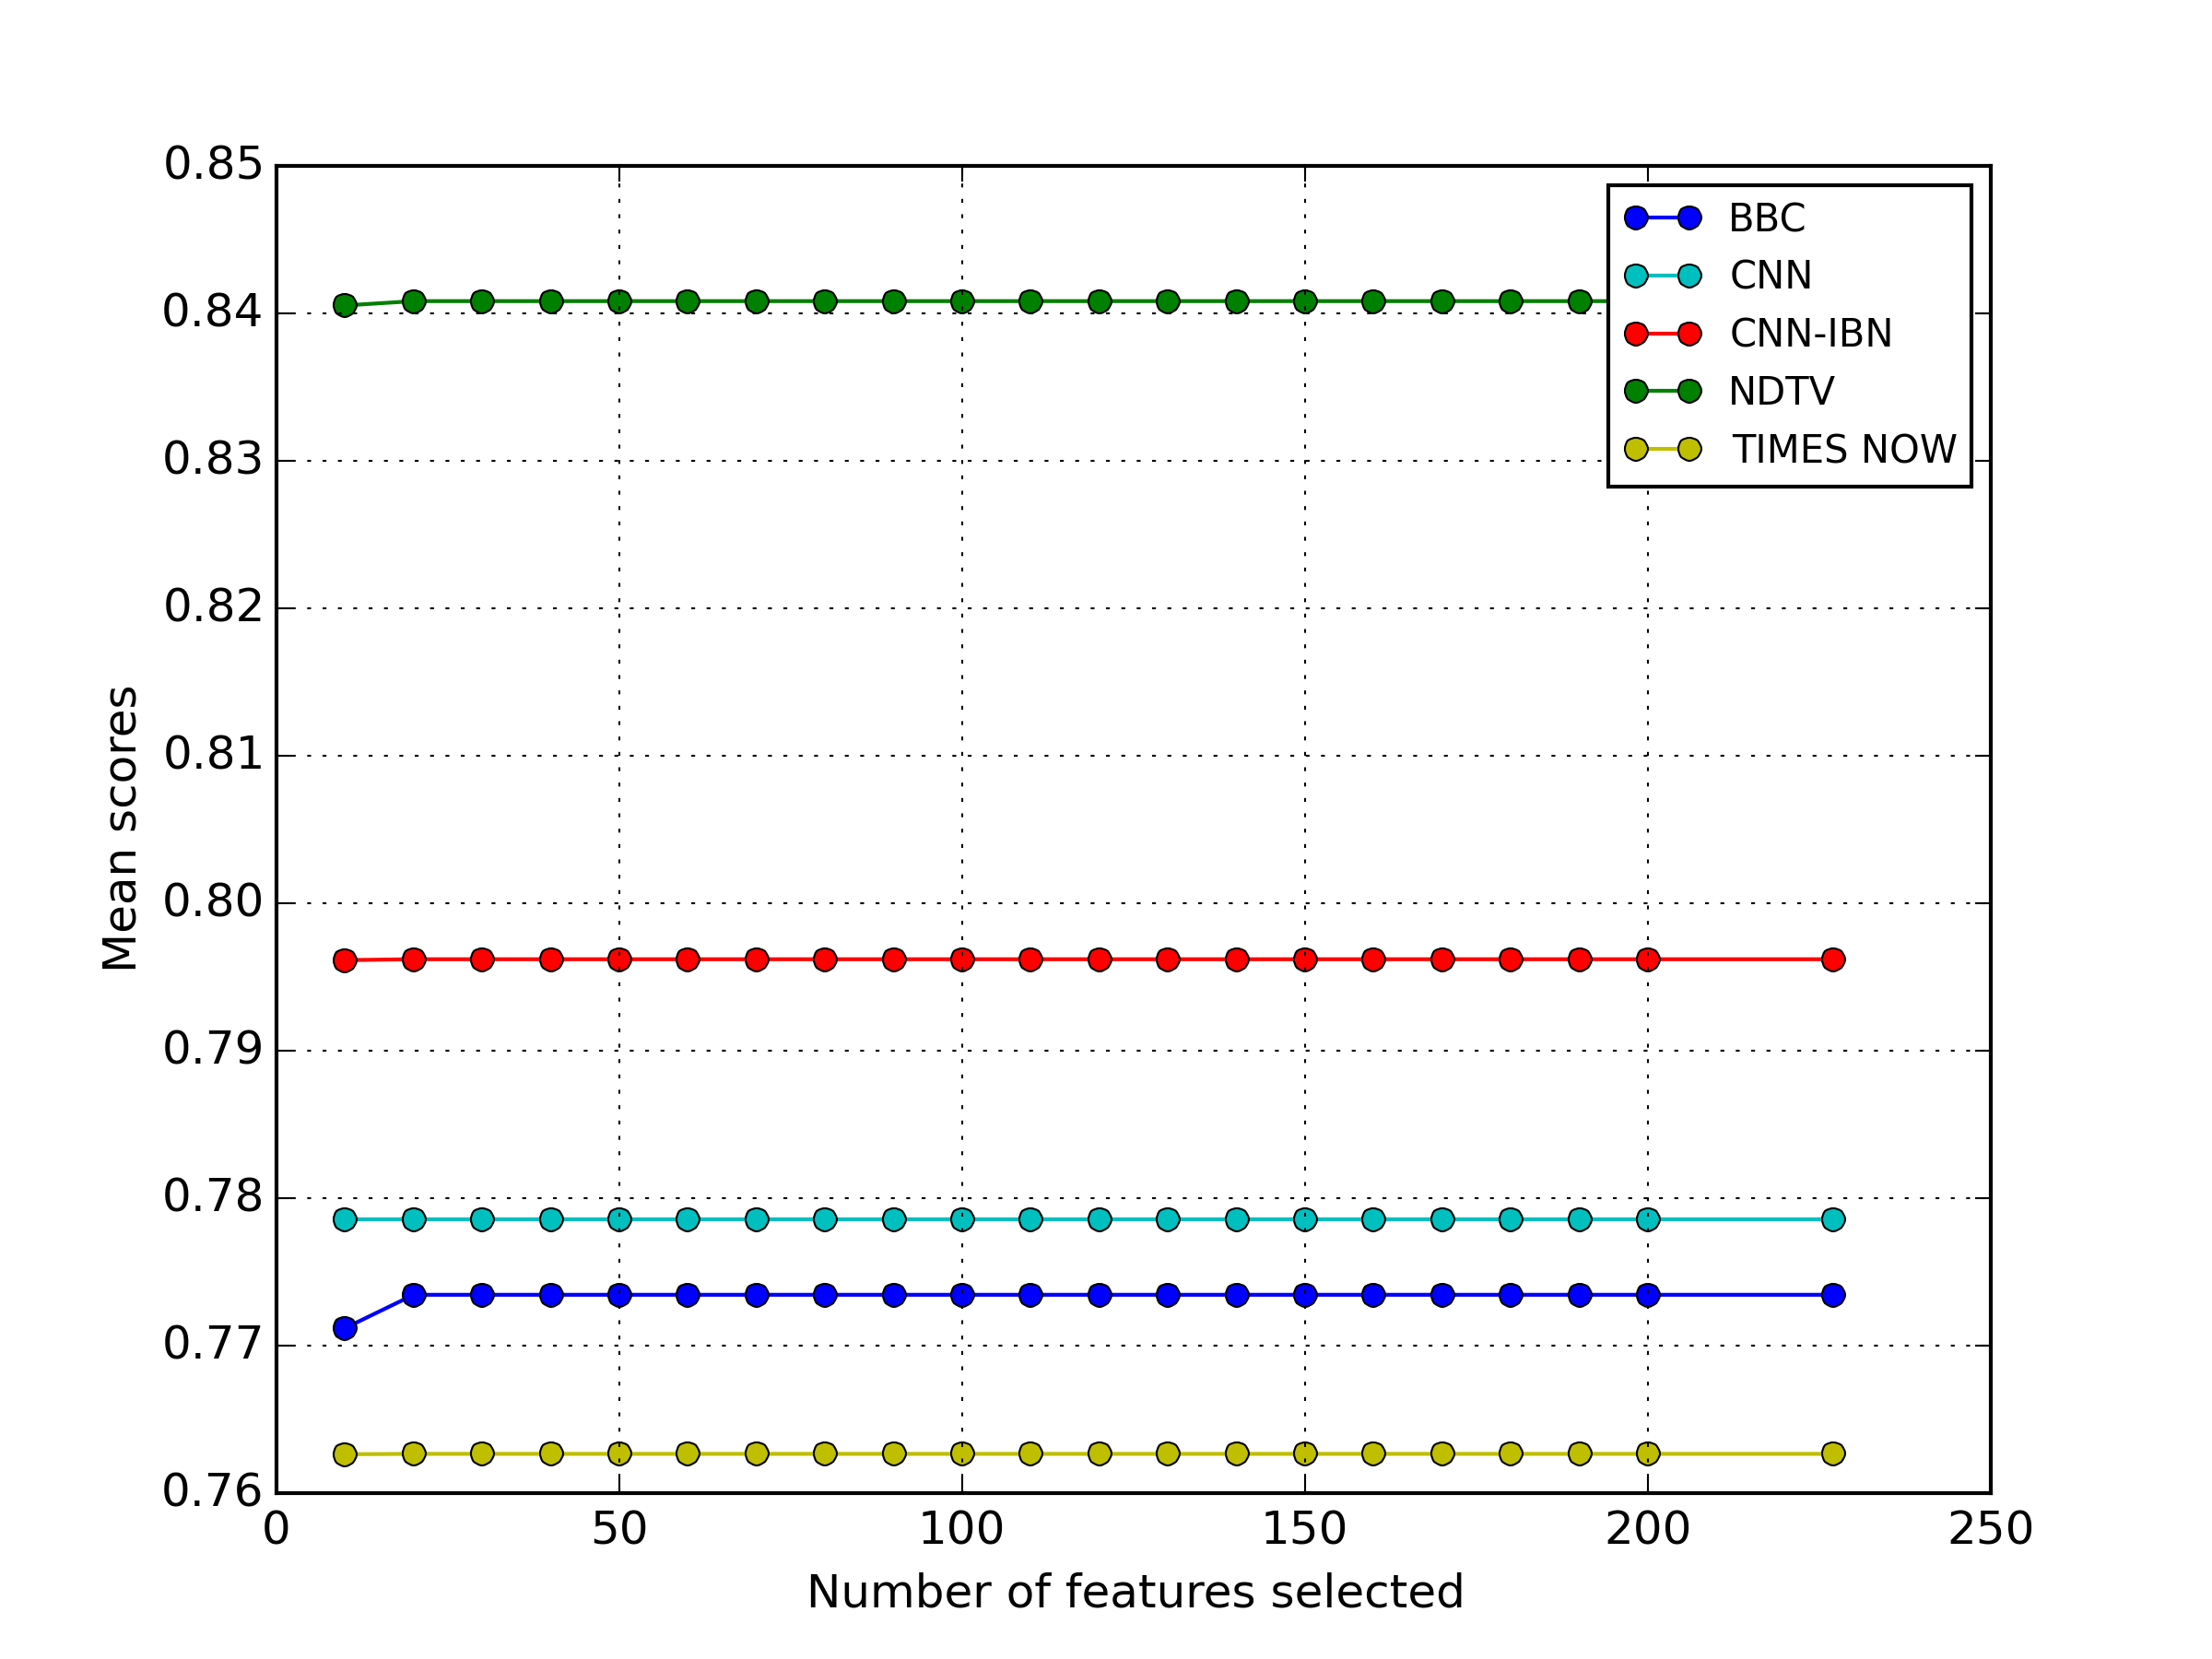
\includegraphics[width=0.5\textwidth]{images/PCA-kNN.png}
    \caption{\(k\)NN scores with PCA}
    \label{fig:knn_pca_scores}
\end{figure} 
\begin{figure}[h!]
    \centering
    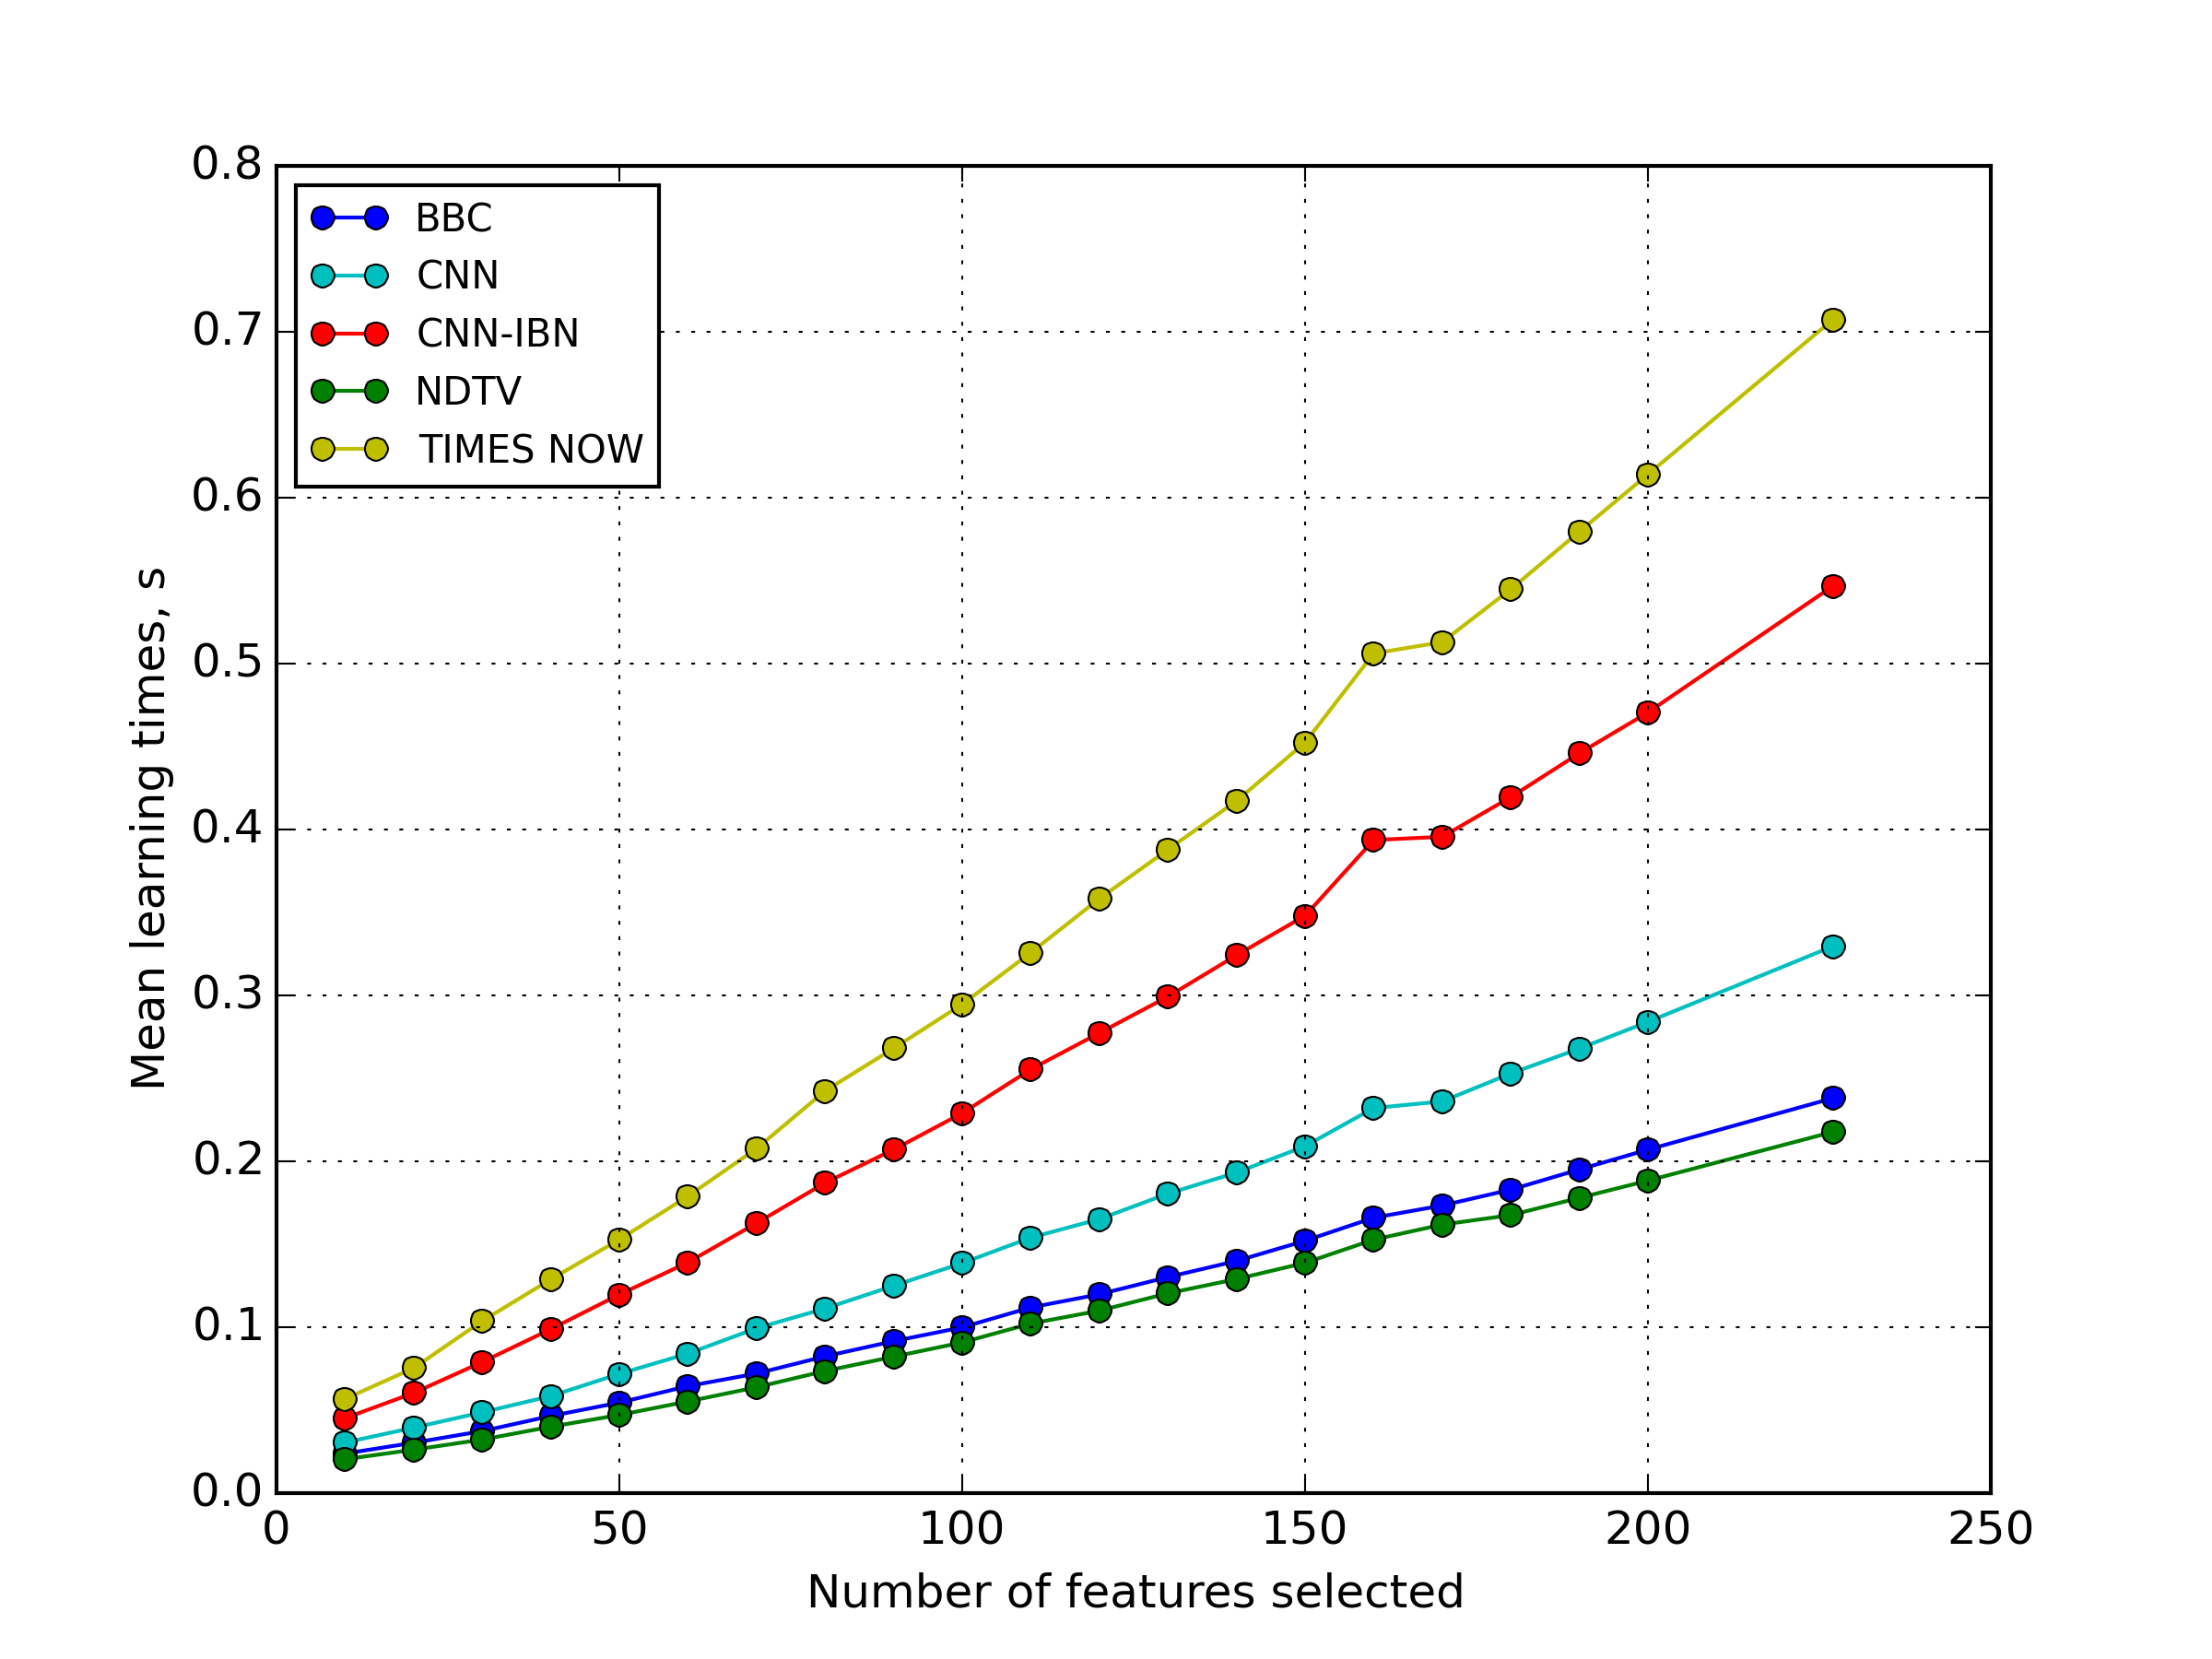
\includegraphics[width=0.5\textwidth]{images/PCA-kNNTime.png}
    \caption{\(k\)NN learning times with PCA}
    \label{fig:knn_pca_times}
\end{figure} 
\par
Линейный дискриминантынй анализ в сочетании с PCA показал ухудшение результатов. Время обучения этого метода мало, так что редукция размерности в данном случае оказалась бесполезной.

\begin{figure}[h!]
    \centering
    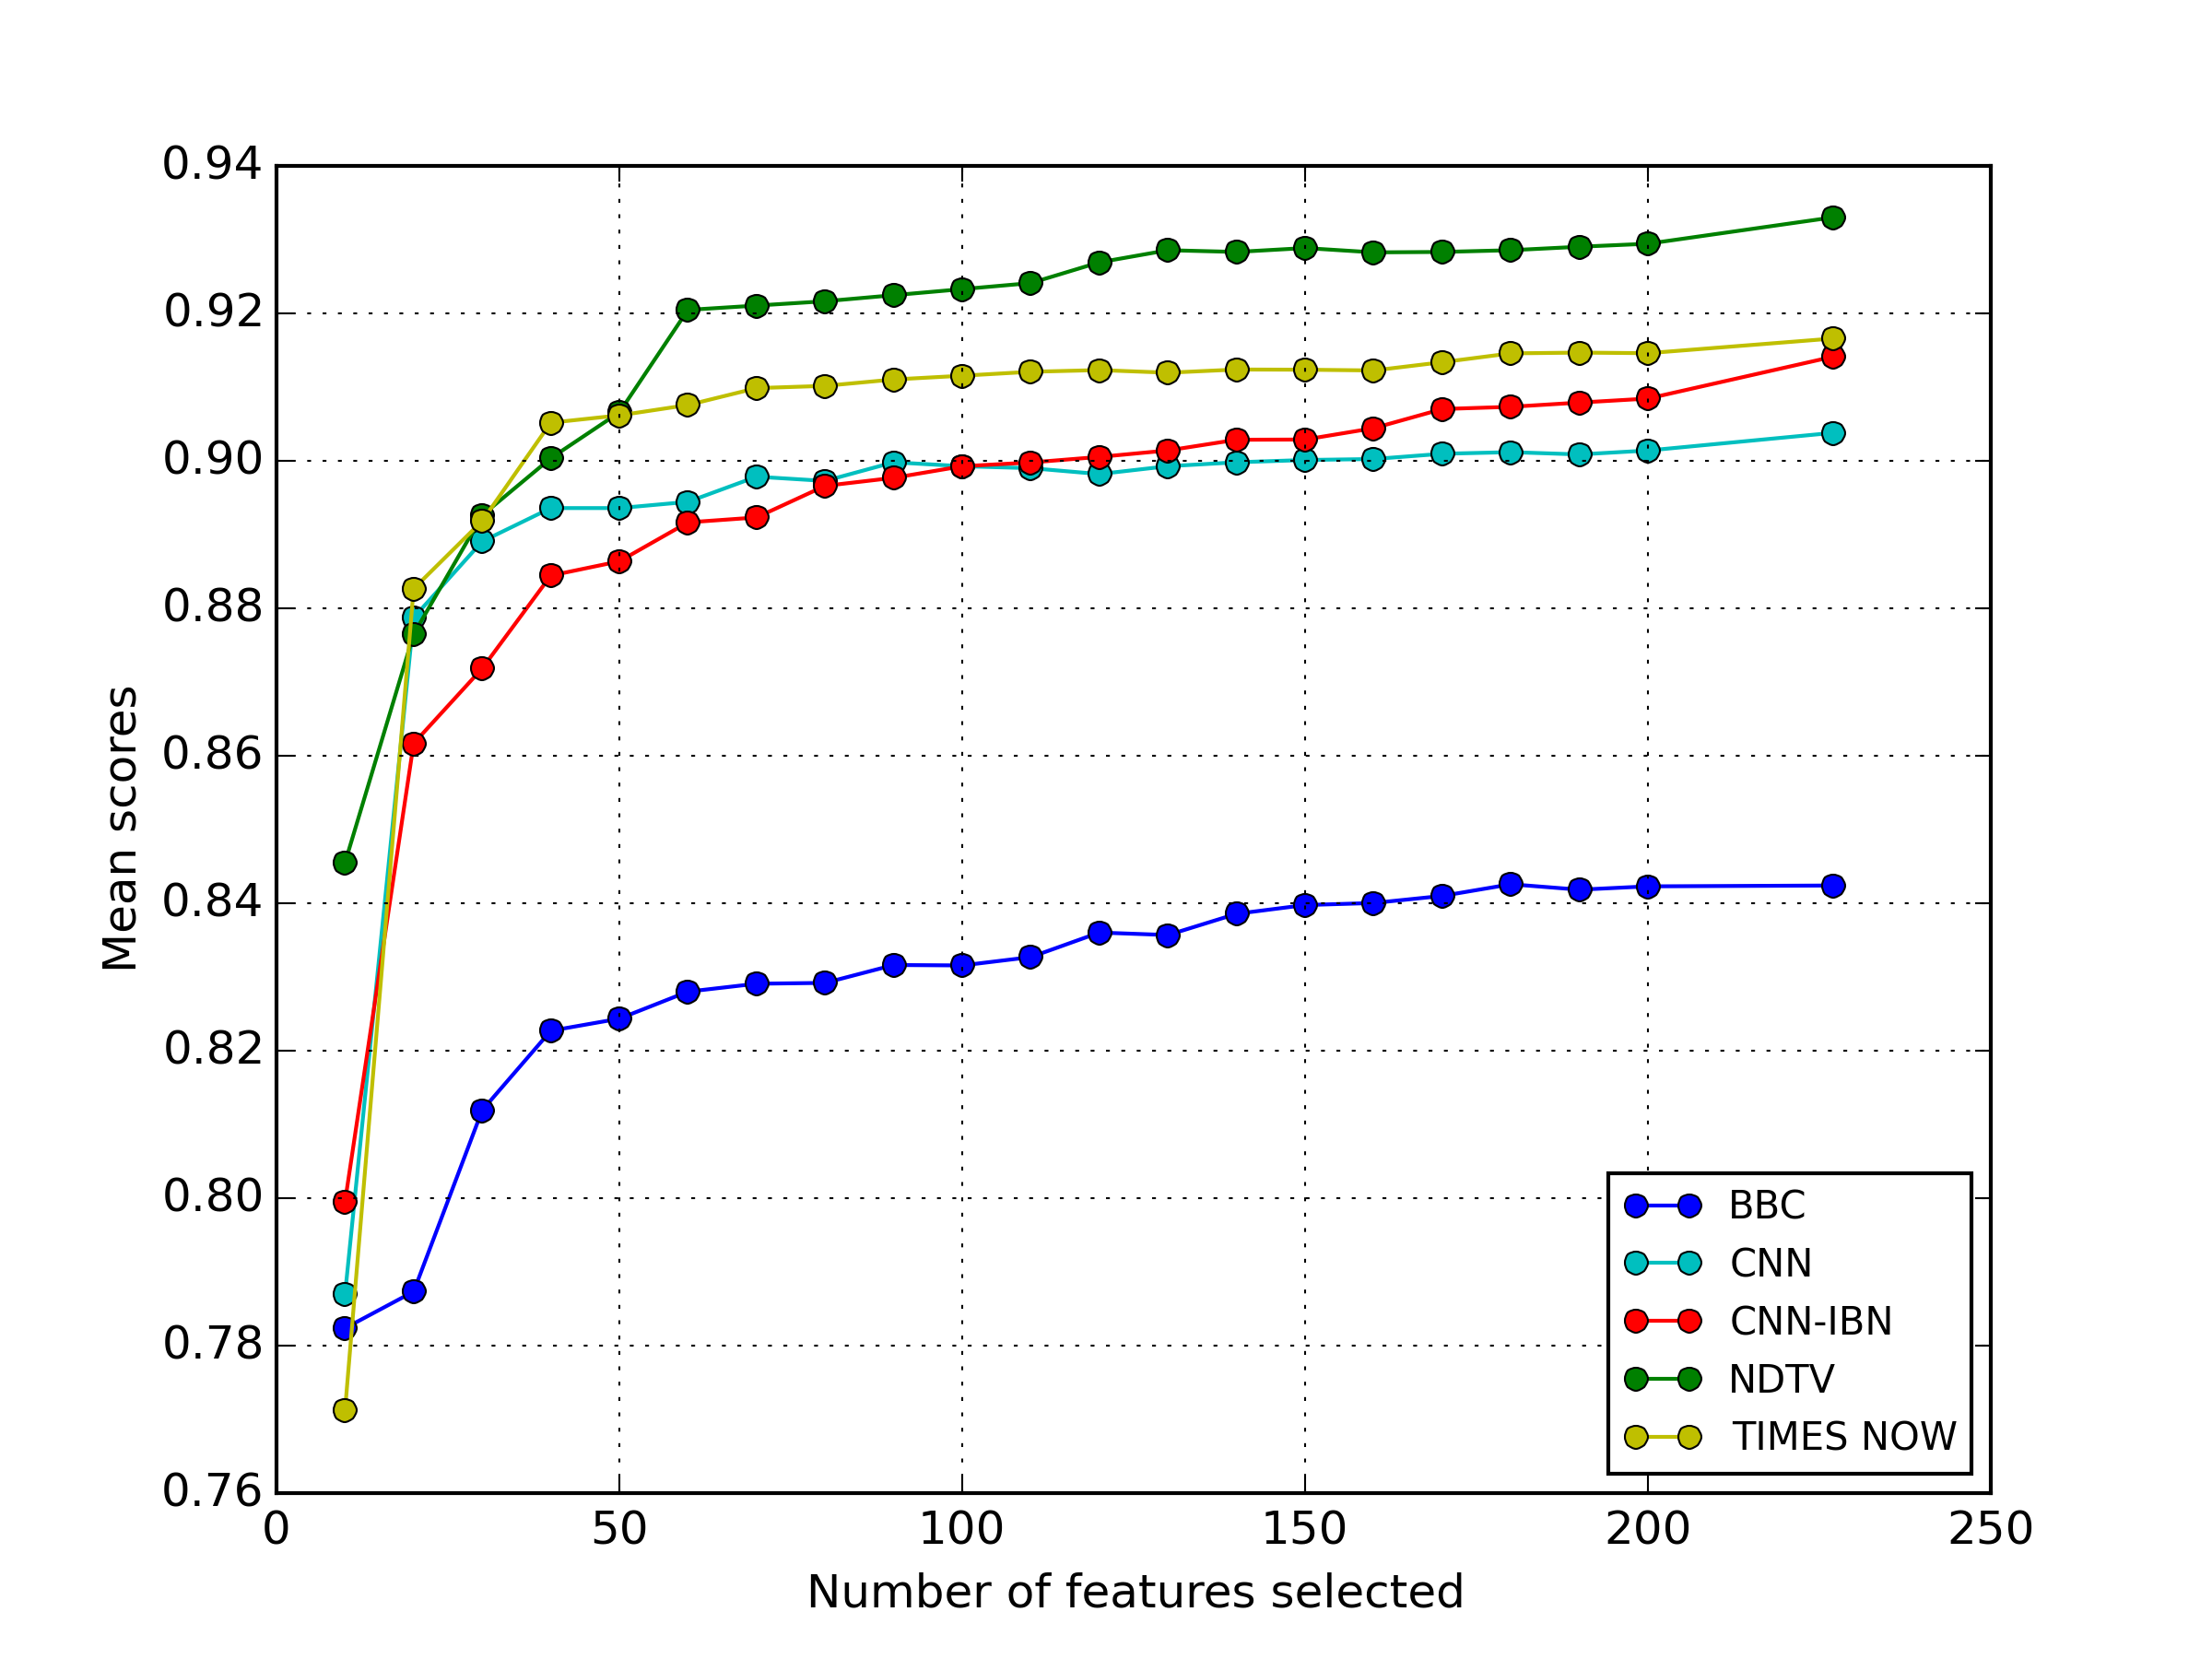
\includegraphics[width=0.5\textwidth]{images/PCA-LDA.png}
    \caption{LDA scores with PCA}
    \label{fig:lda_pca_scores}
\end{figure} 
\begin{figure}[h!]
    \centering
    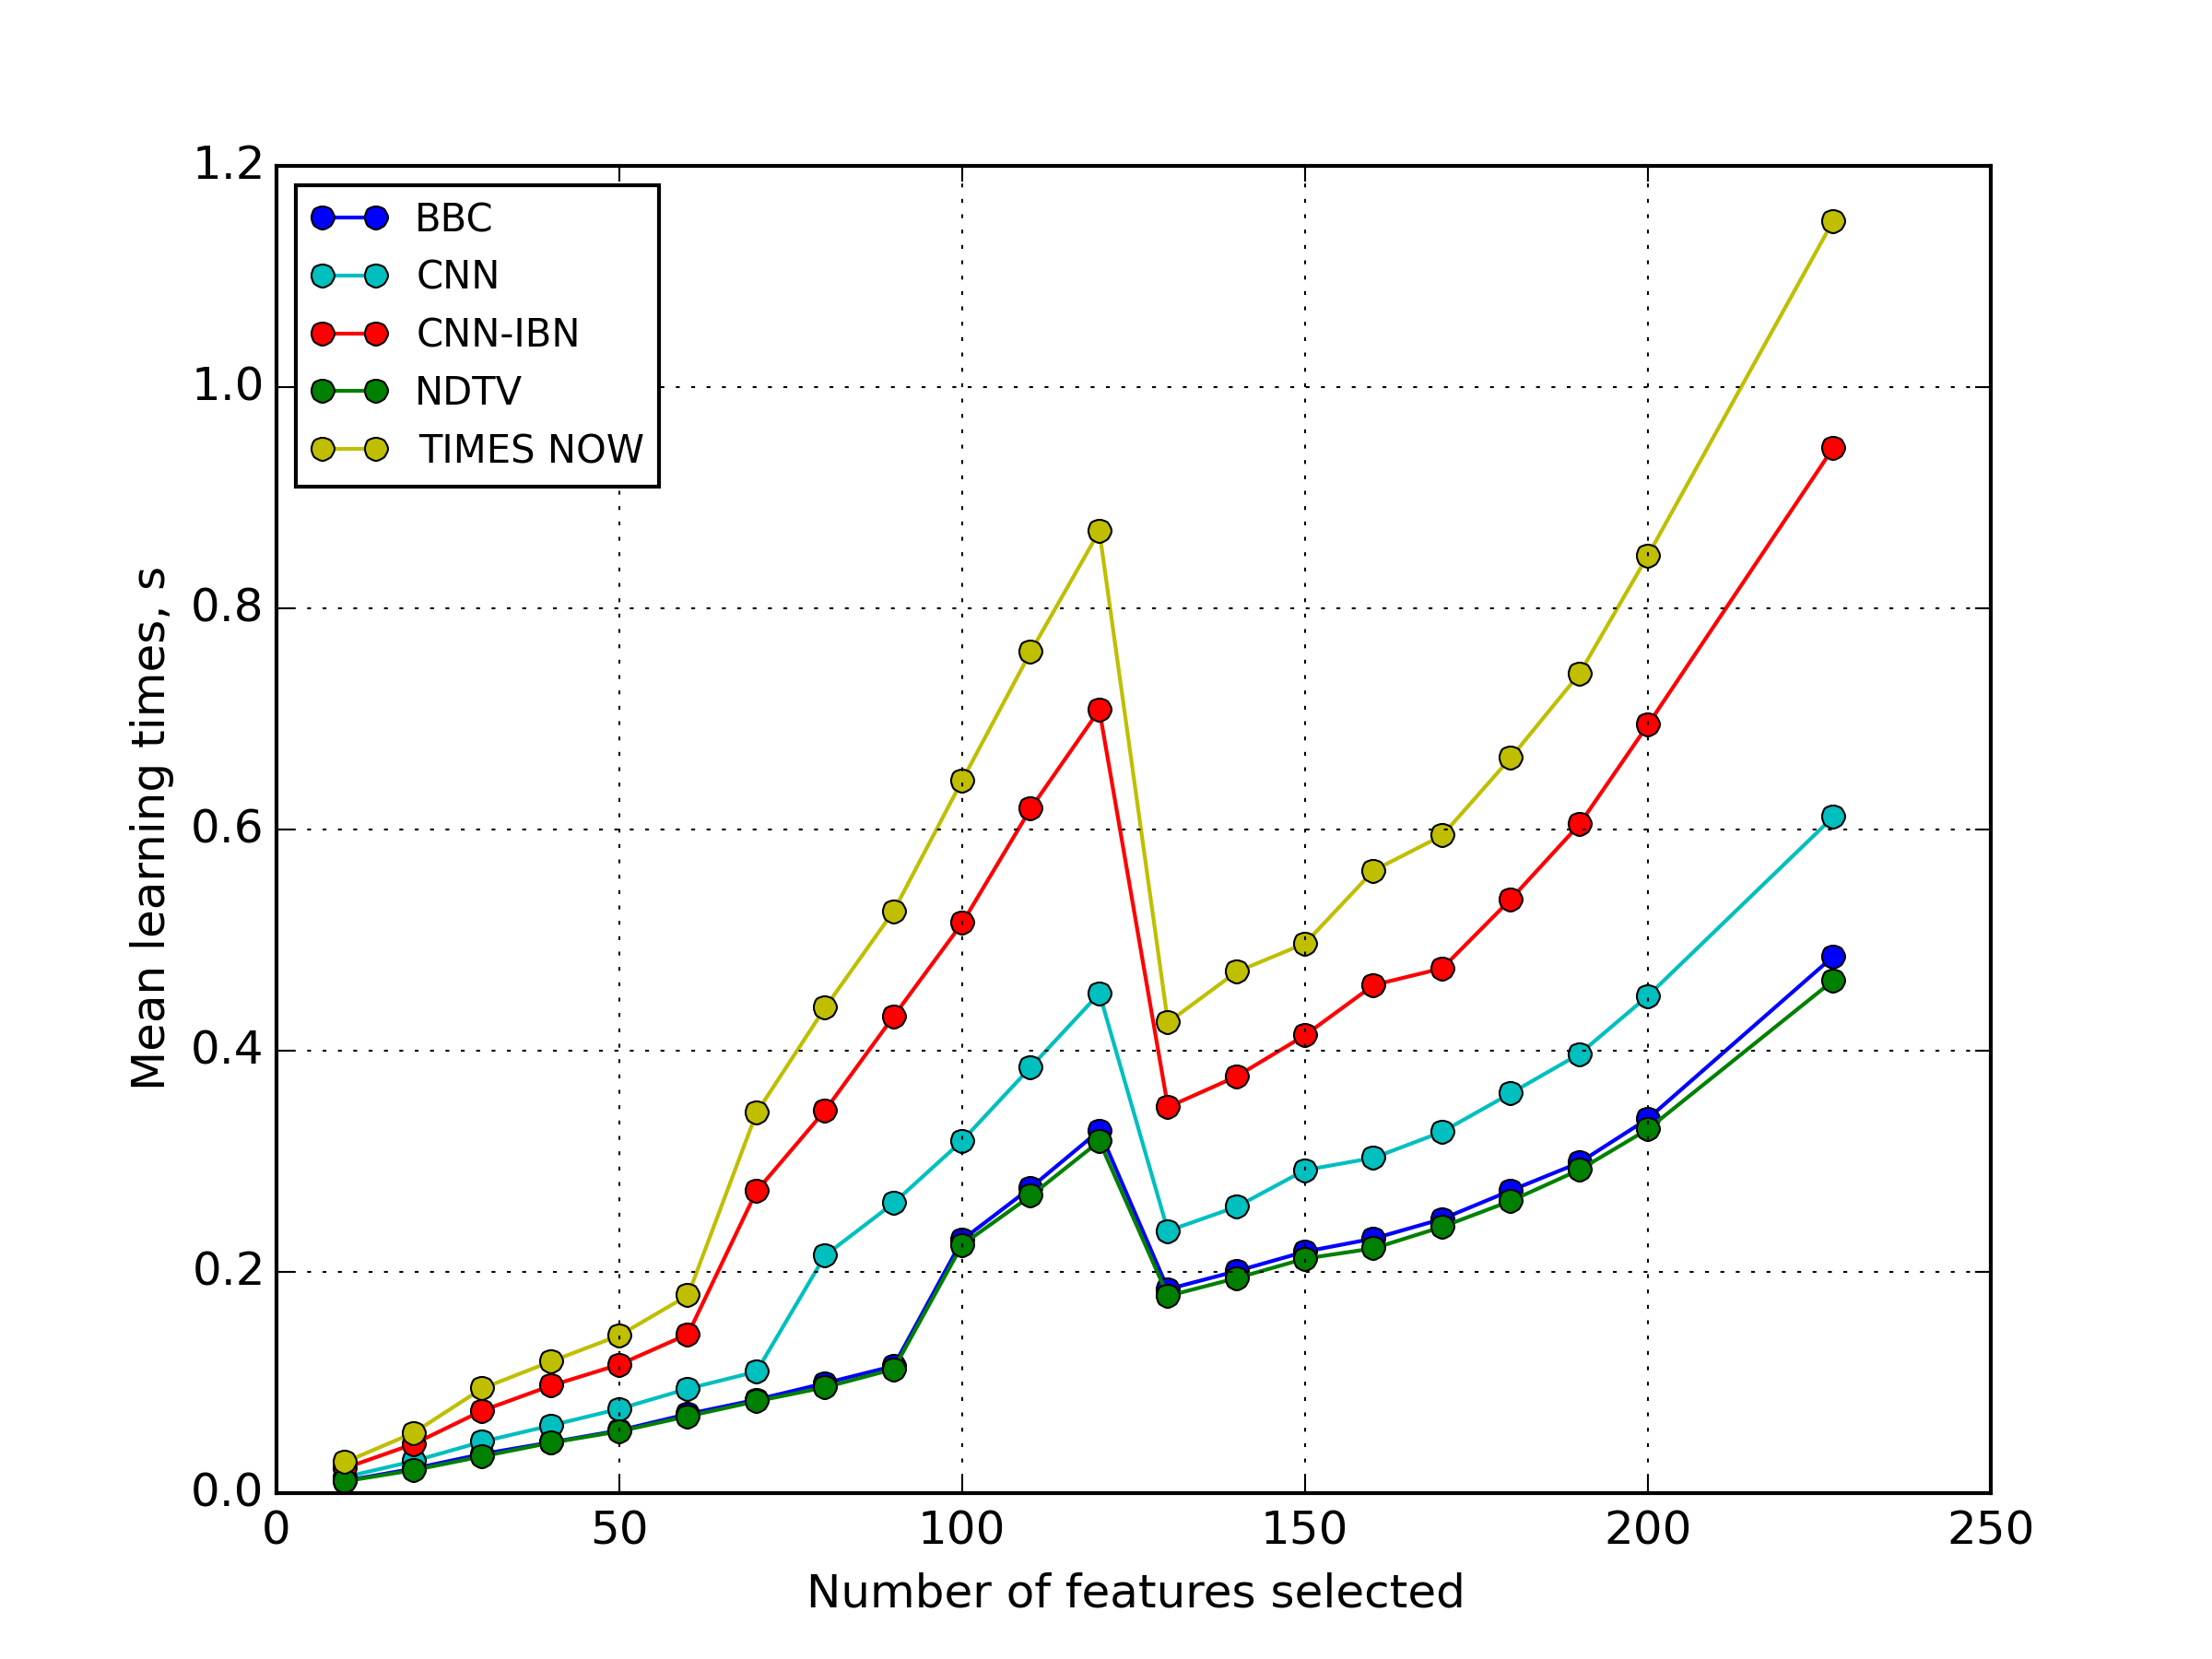
\includegraphics[width=0.5\textwidth]{images/PCA-LDATime.png}
    \caption{LDA learning times with PCA}
    \label{fig:lda_pca_times}
\end{figure} 
\par
Наилучшего результата с точки зрения качества классификации удалось достичь с помощью машины опорных векторов и снижения размерности до 50 или 60, в зависимости от канала. Кроме того, при меньшей размерности значительно падает время работы SVM.

\begin{figure}[h!]
    \centering
    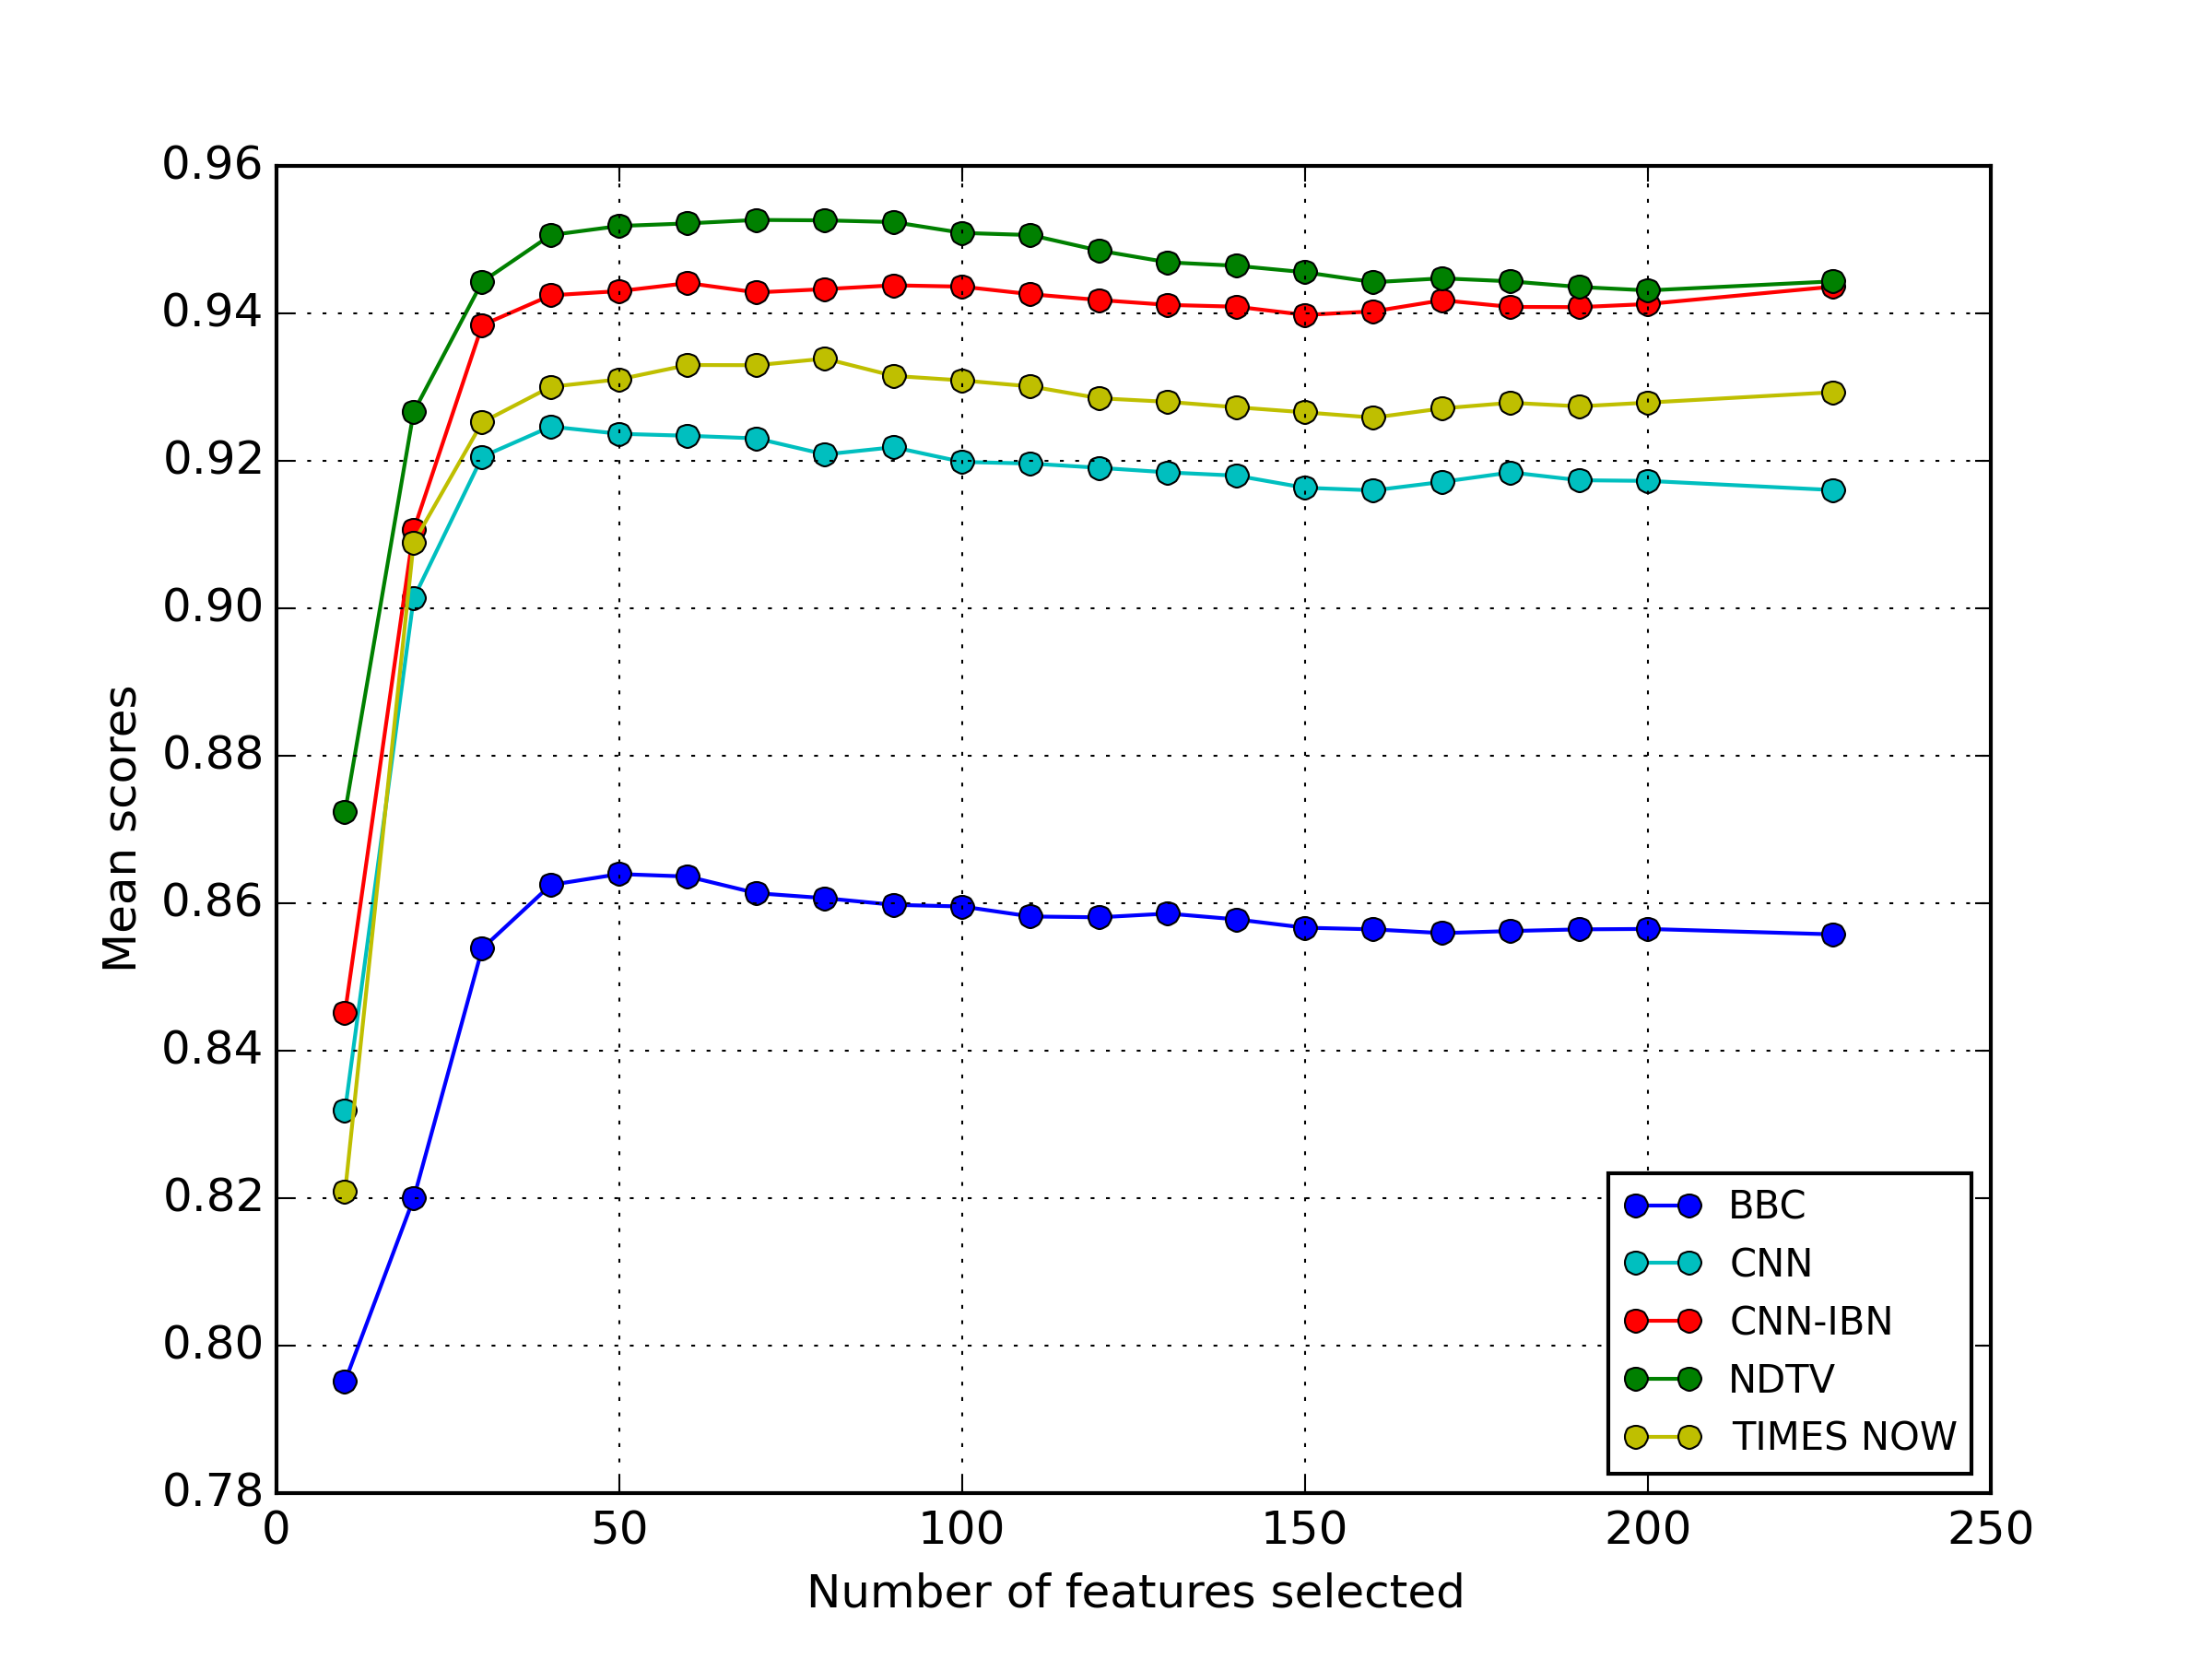
\includegraphics[width=0.5\textwidth]{images/PCA-SVM.png}
    \caption{SVM scores with PCA}
    \label{fig:svm_pca_scores}
\end{figure} 
\begin{figure}[h!]
    \centering
    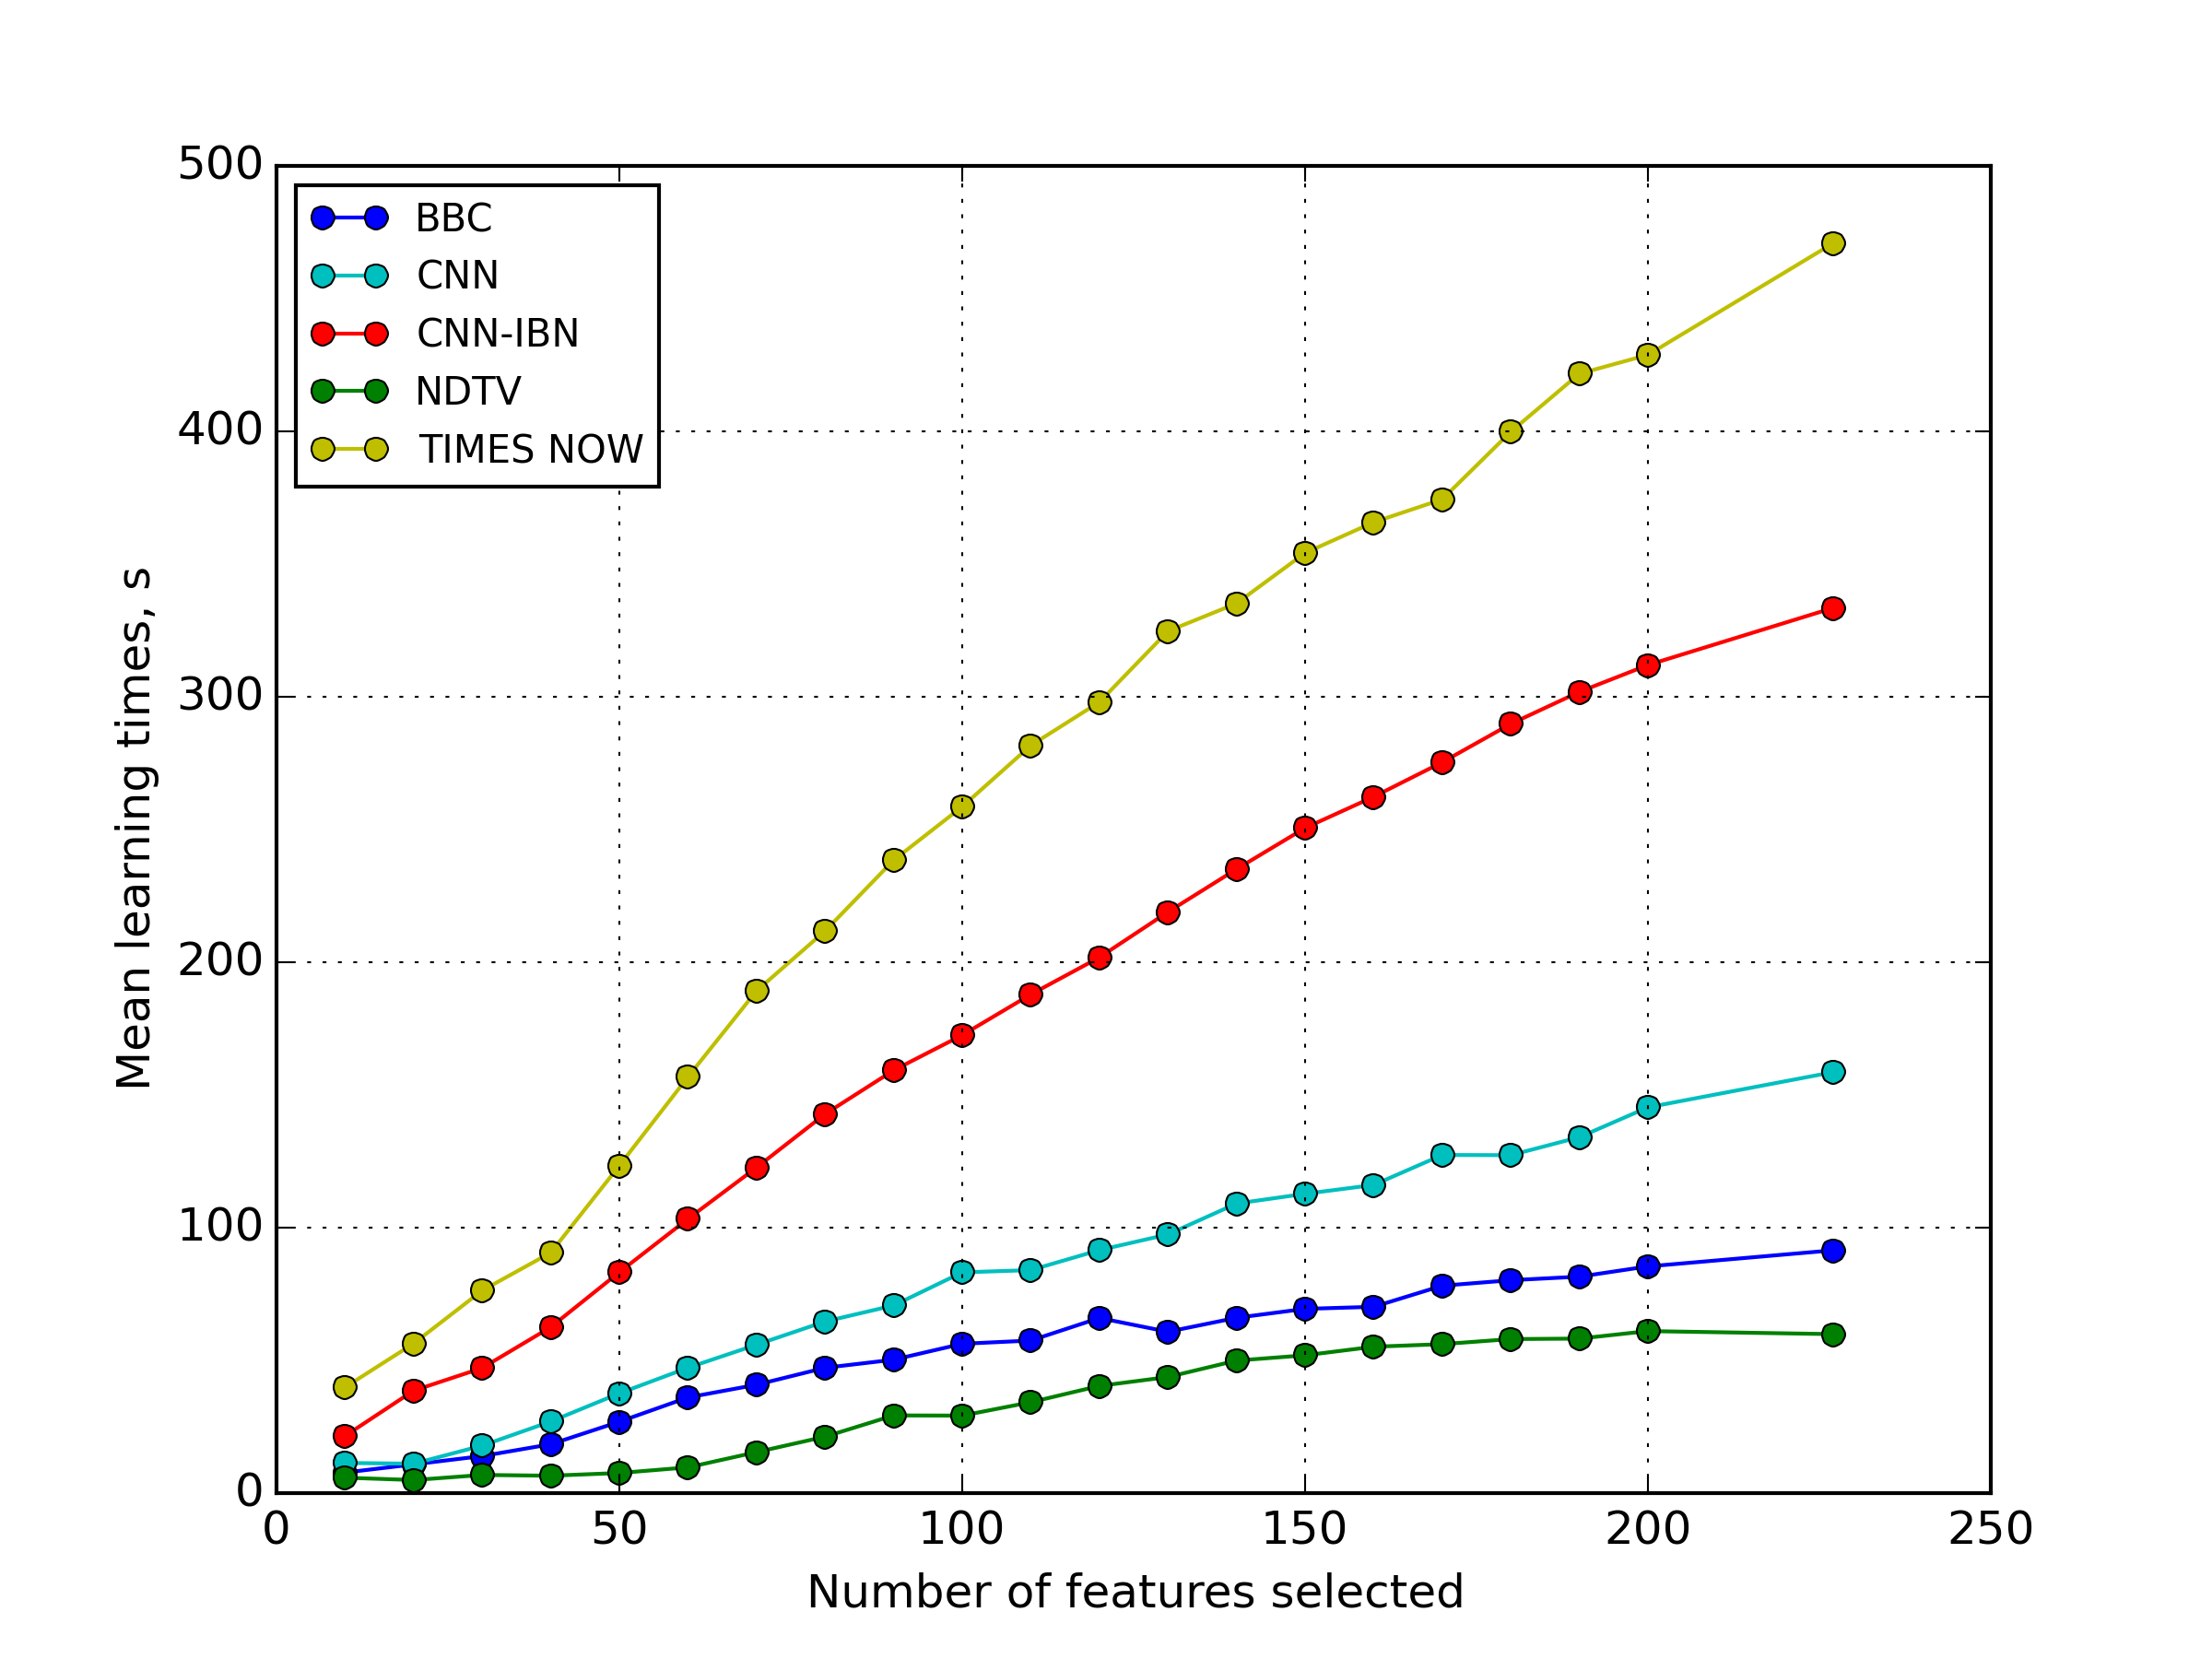
\includegraphics[width=0.5\textwidth]{images/PCA-SVMTime.png}
    \caption{SVM learning times with PCA}
    \label{fig:svm_pca_times}
\end{figure} 
\par
 Хорошие результаты при уменьшении размерности с помошью PCA показал алгоритм random forest. С уменьшением размерности задачи растёт доля верных предсказаний (на рис. \ref{fig:randfor_pca_scores} показаны графики 
 зависимости качества обучения алгоритма на разных каналах).
 При одновременном улучшении результата кросс-валидации практически линейно уменьшается время обучения алгоритма (рис. \ref{fig:randfor_pca_times}). Оптимальное число признаков для алгоритма random forest с точки зрения сочетания качества обучения и затраченного времени --- 50 или 60 в зависимости от канала.
 
\begin{figure}[h!]
    \centering
    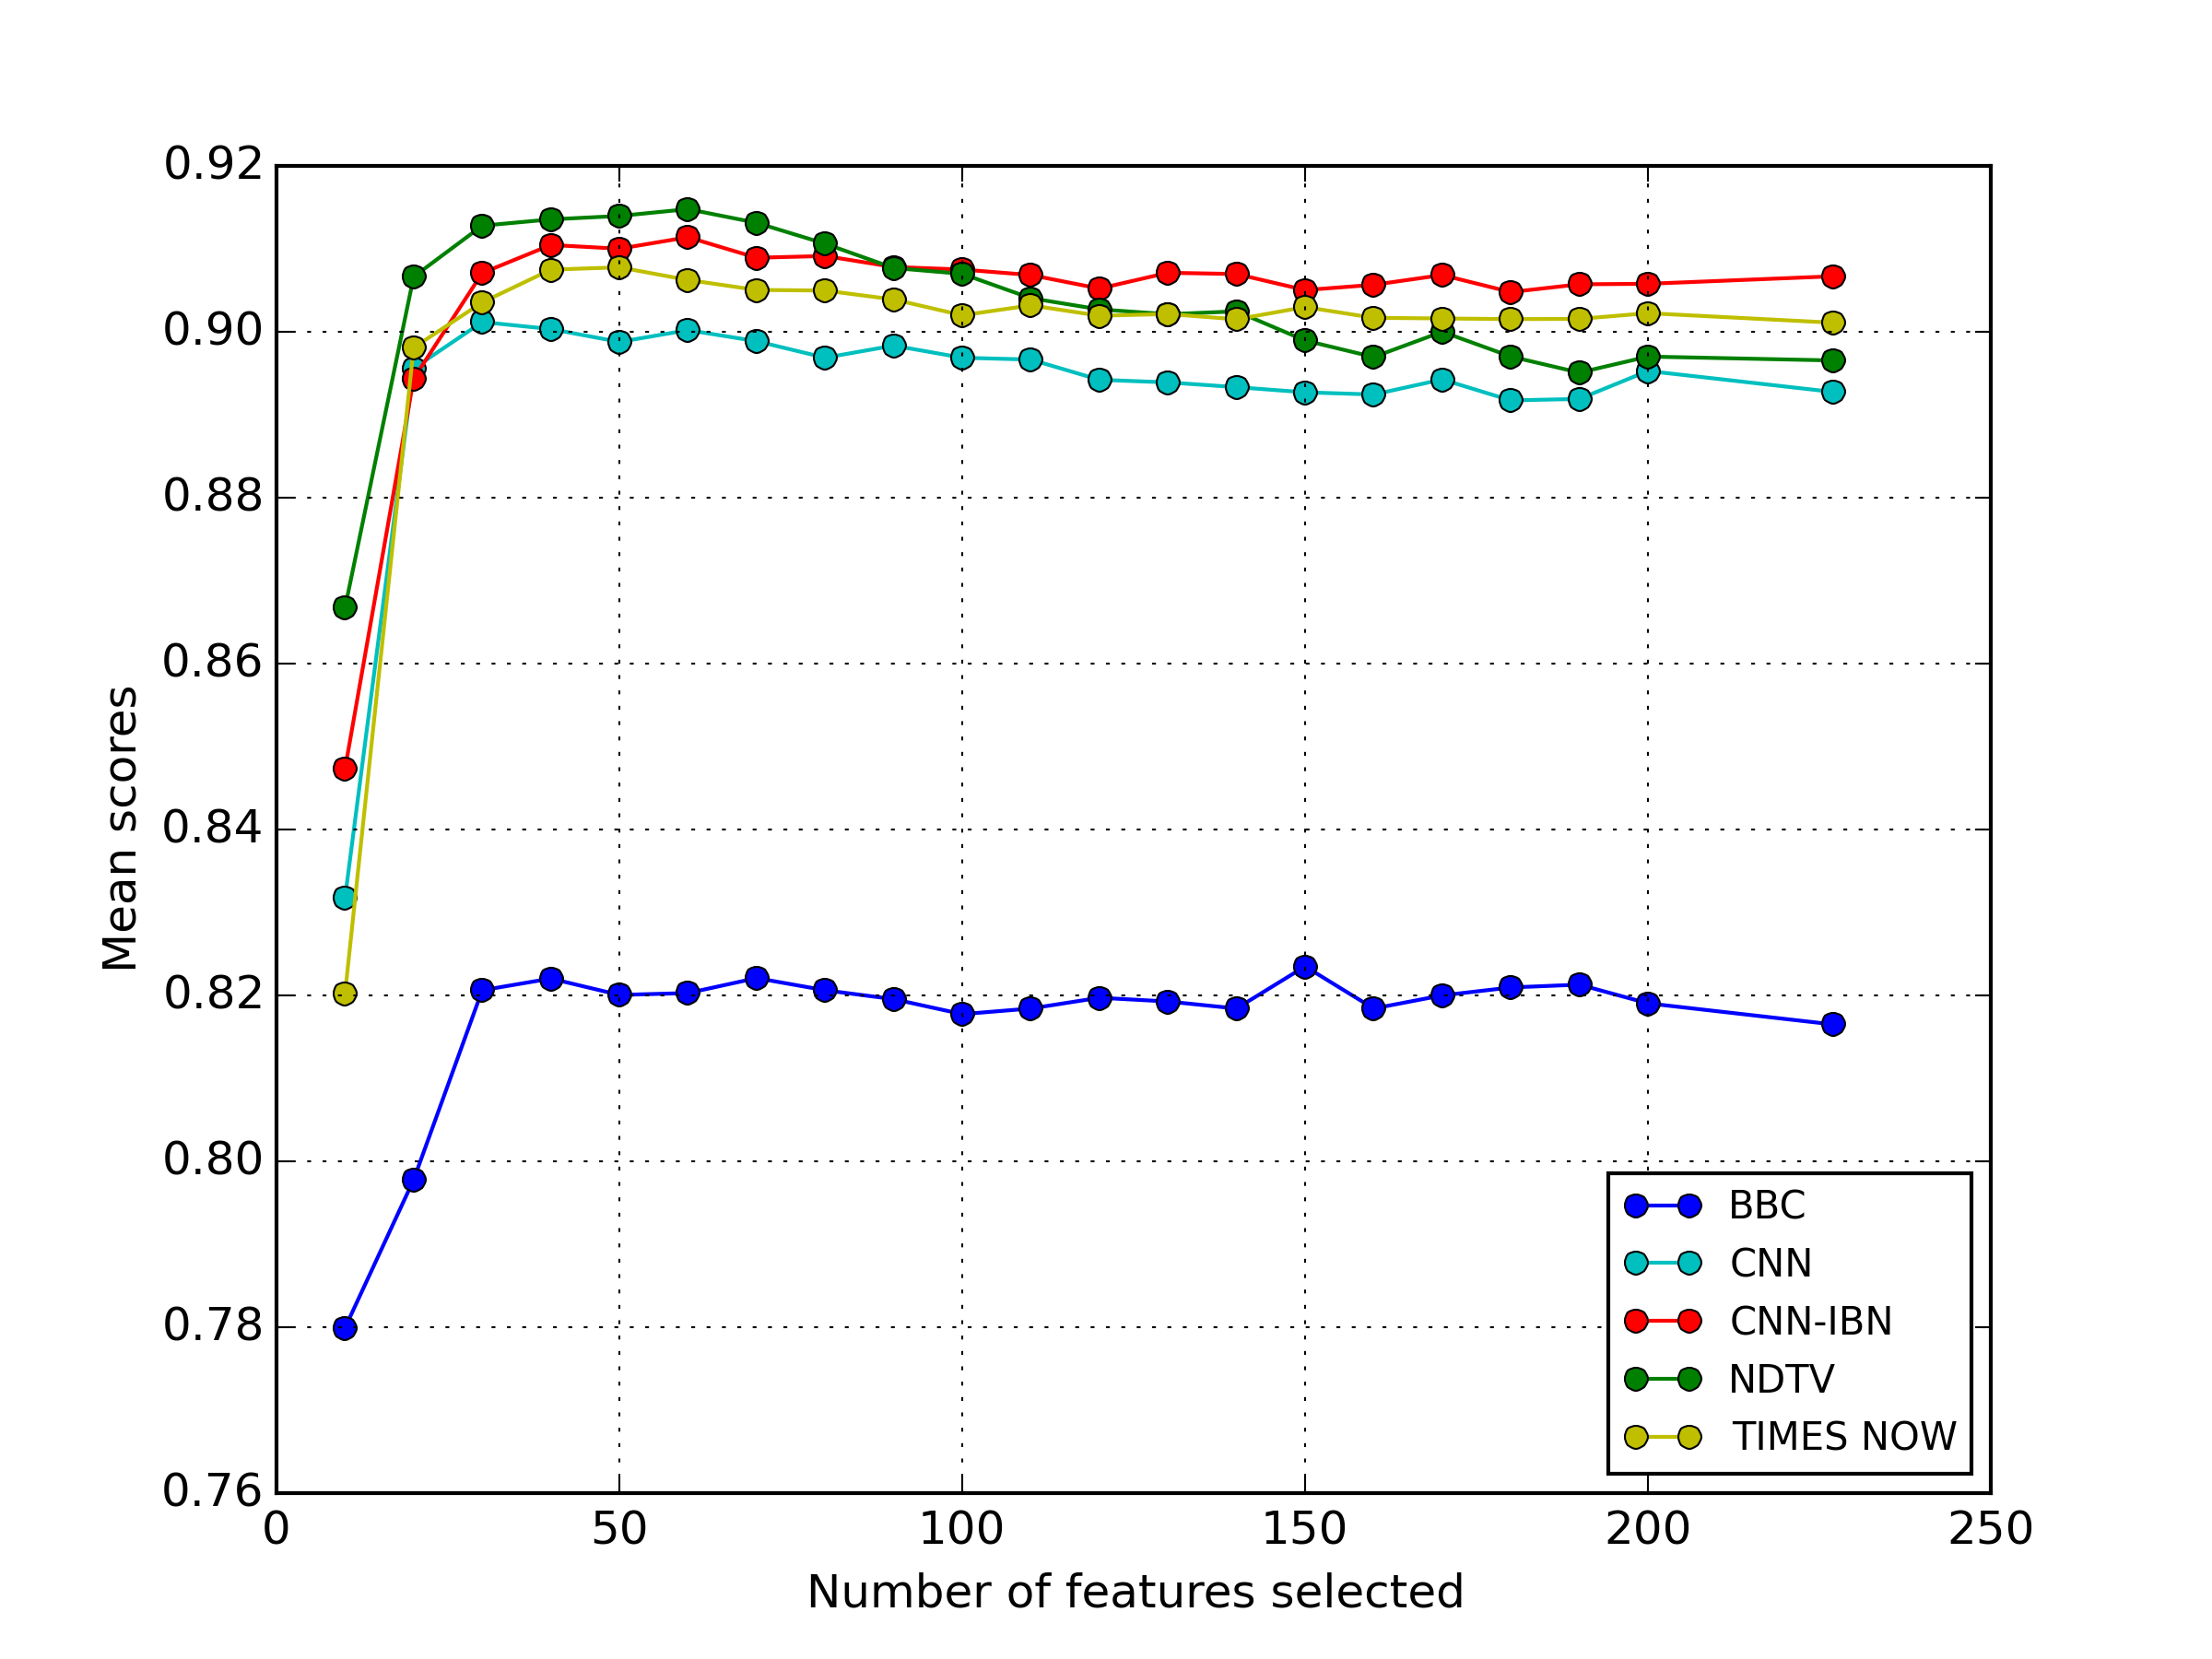
\includegraphics[width=0.5\textwidth]{images/PCA-randfor.png}
    \caption{Random forest scores with PCA}
    \label{fig:randfor_pca_scores}
\end{figure} 
 
 \begin{figure}[h!]
    \centering
    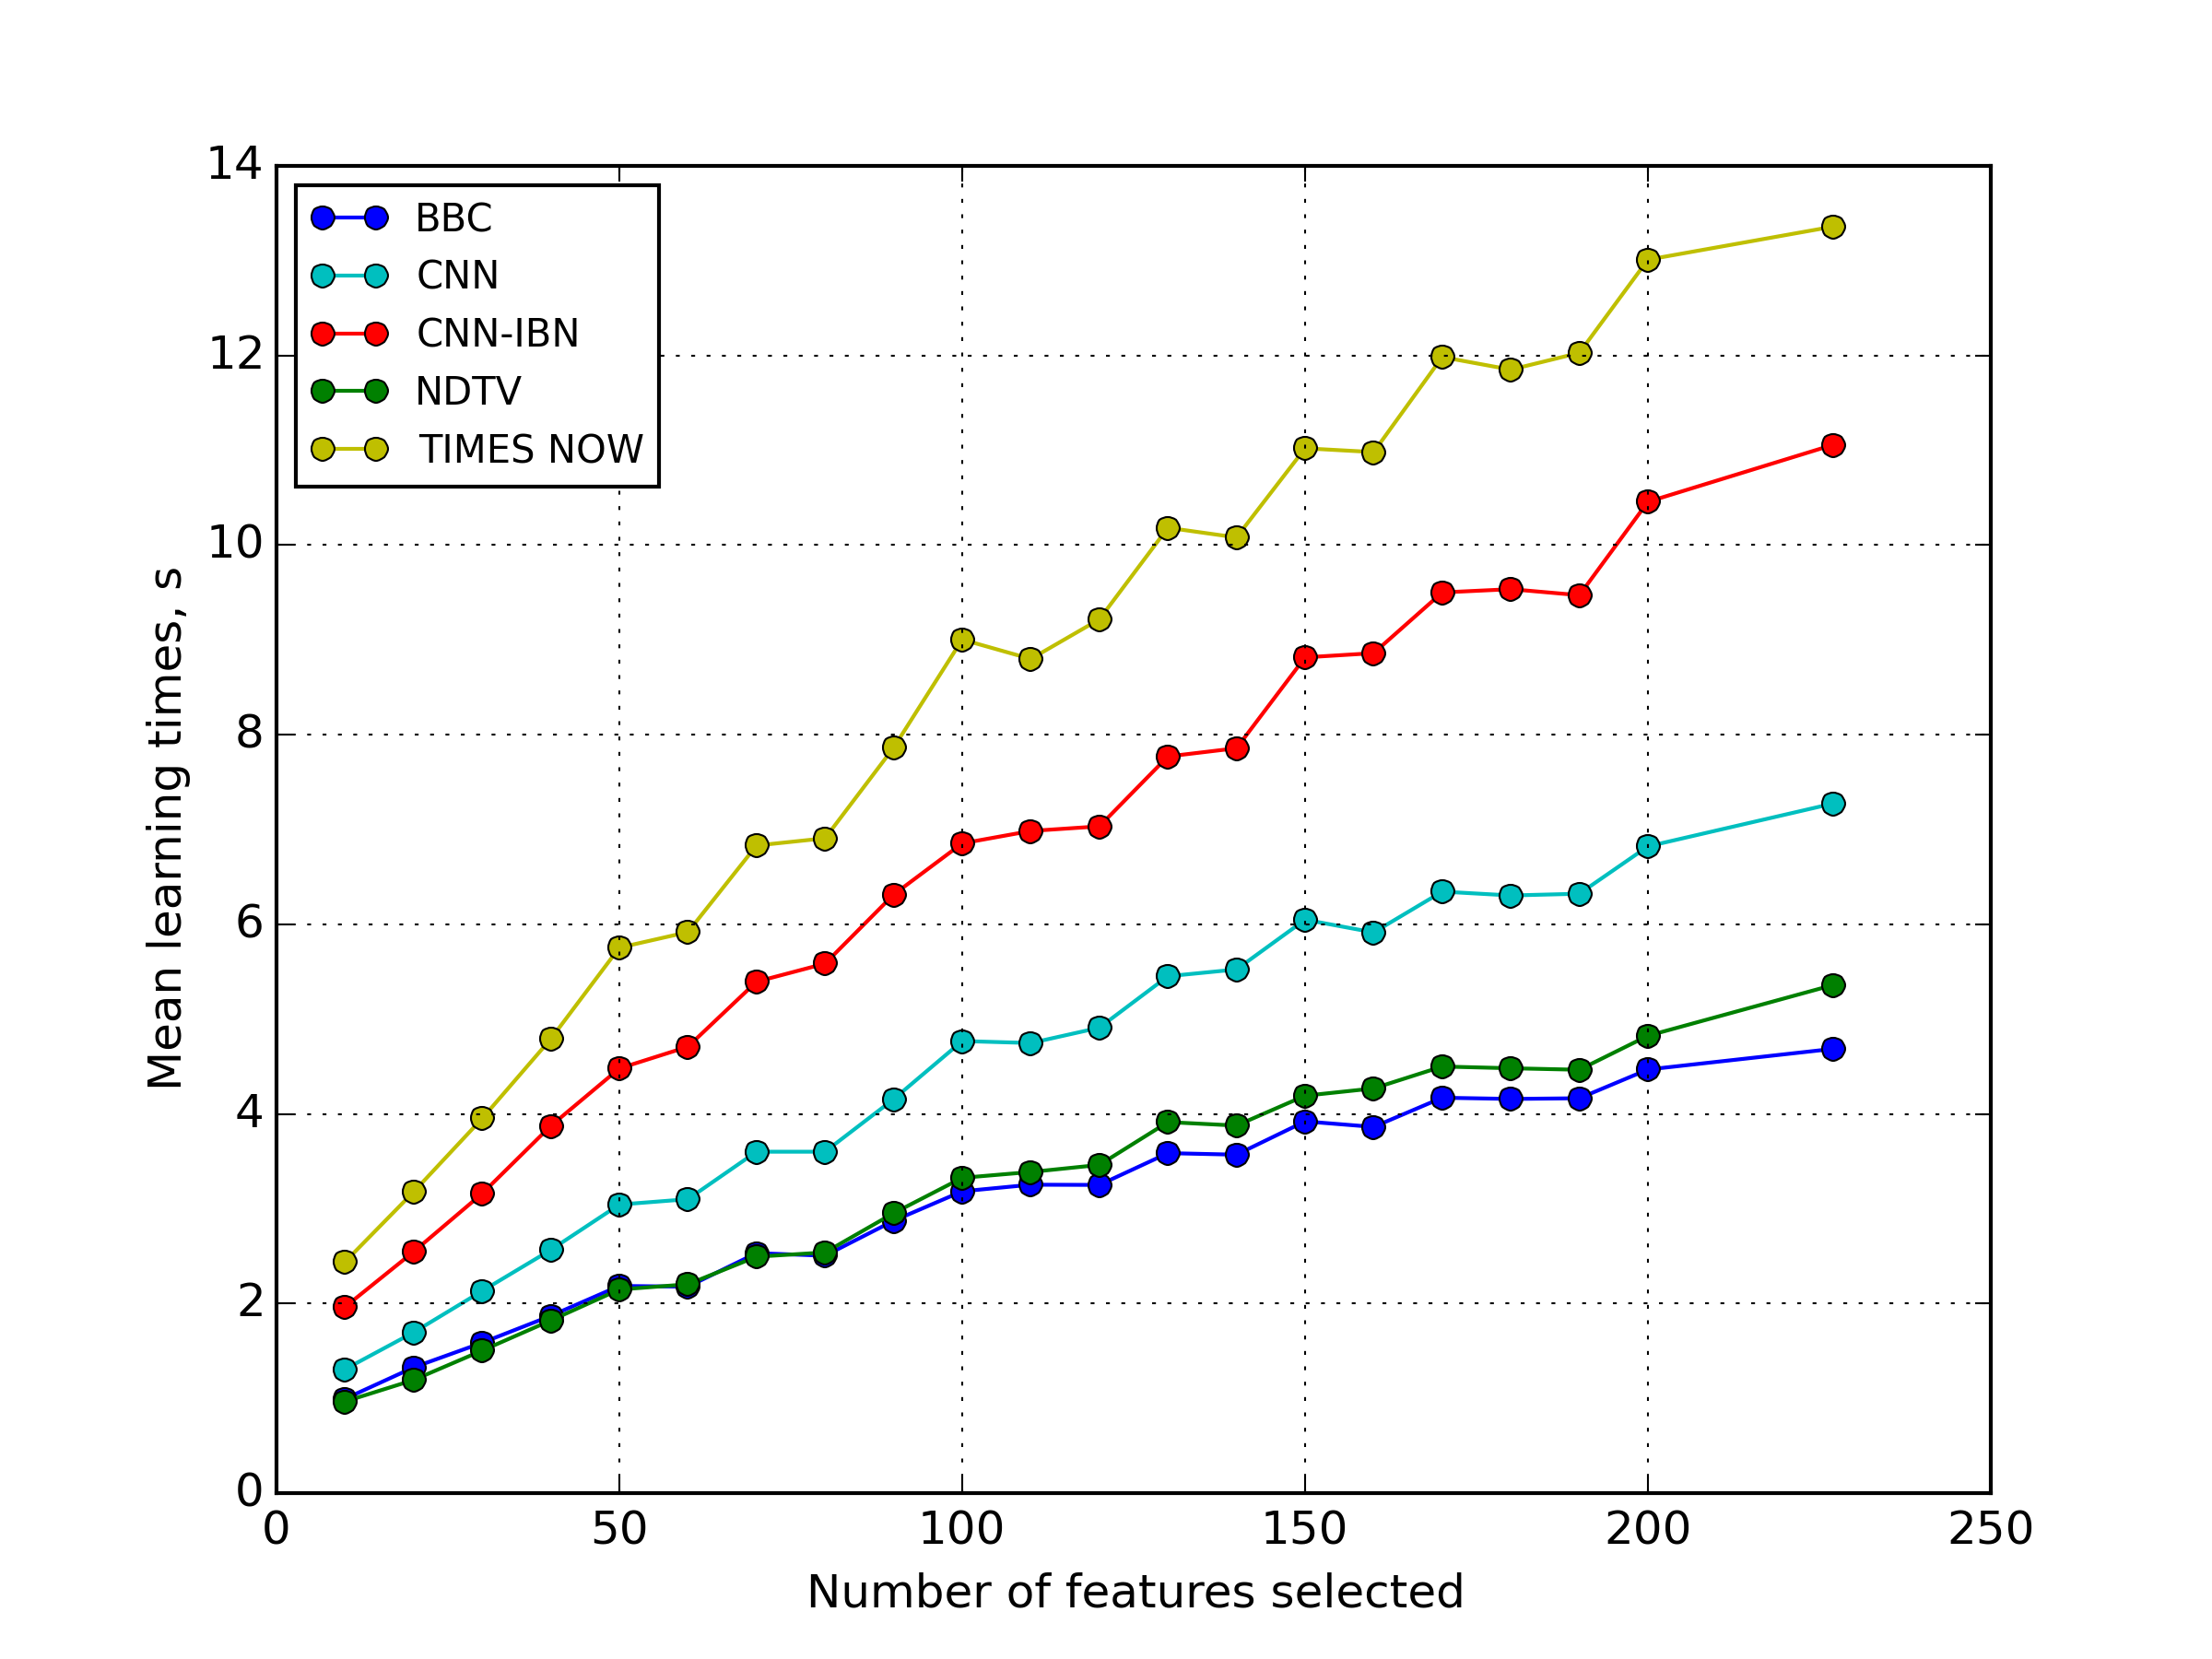
\includegraphics[width=0.5\textwidth]{images/PCA-randforTime.png}
    \caption{Random forest learning times with PCA}
    \label{fig:randfor_pca_times}
\end{figure} 
  \par
  Ещё одним методом, слабо чувствительным к применению PCA стал градиентый бустинг деревьев. PCA в таком случае можно использовать чтобы снизить время обучения модели. Из рис. \ref{fig:gtb_pca_times} можно увидеть, что при снижении размерности данных в 2 раз время обучения падает тоже примерно в 2 раза.

\begin{figure}[h!]
    \centering
    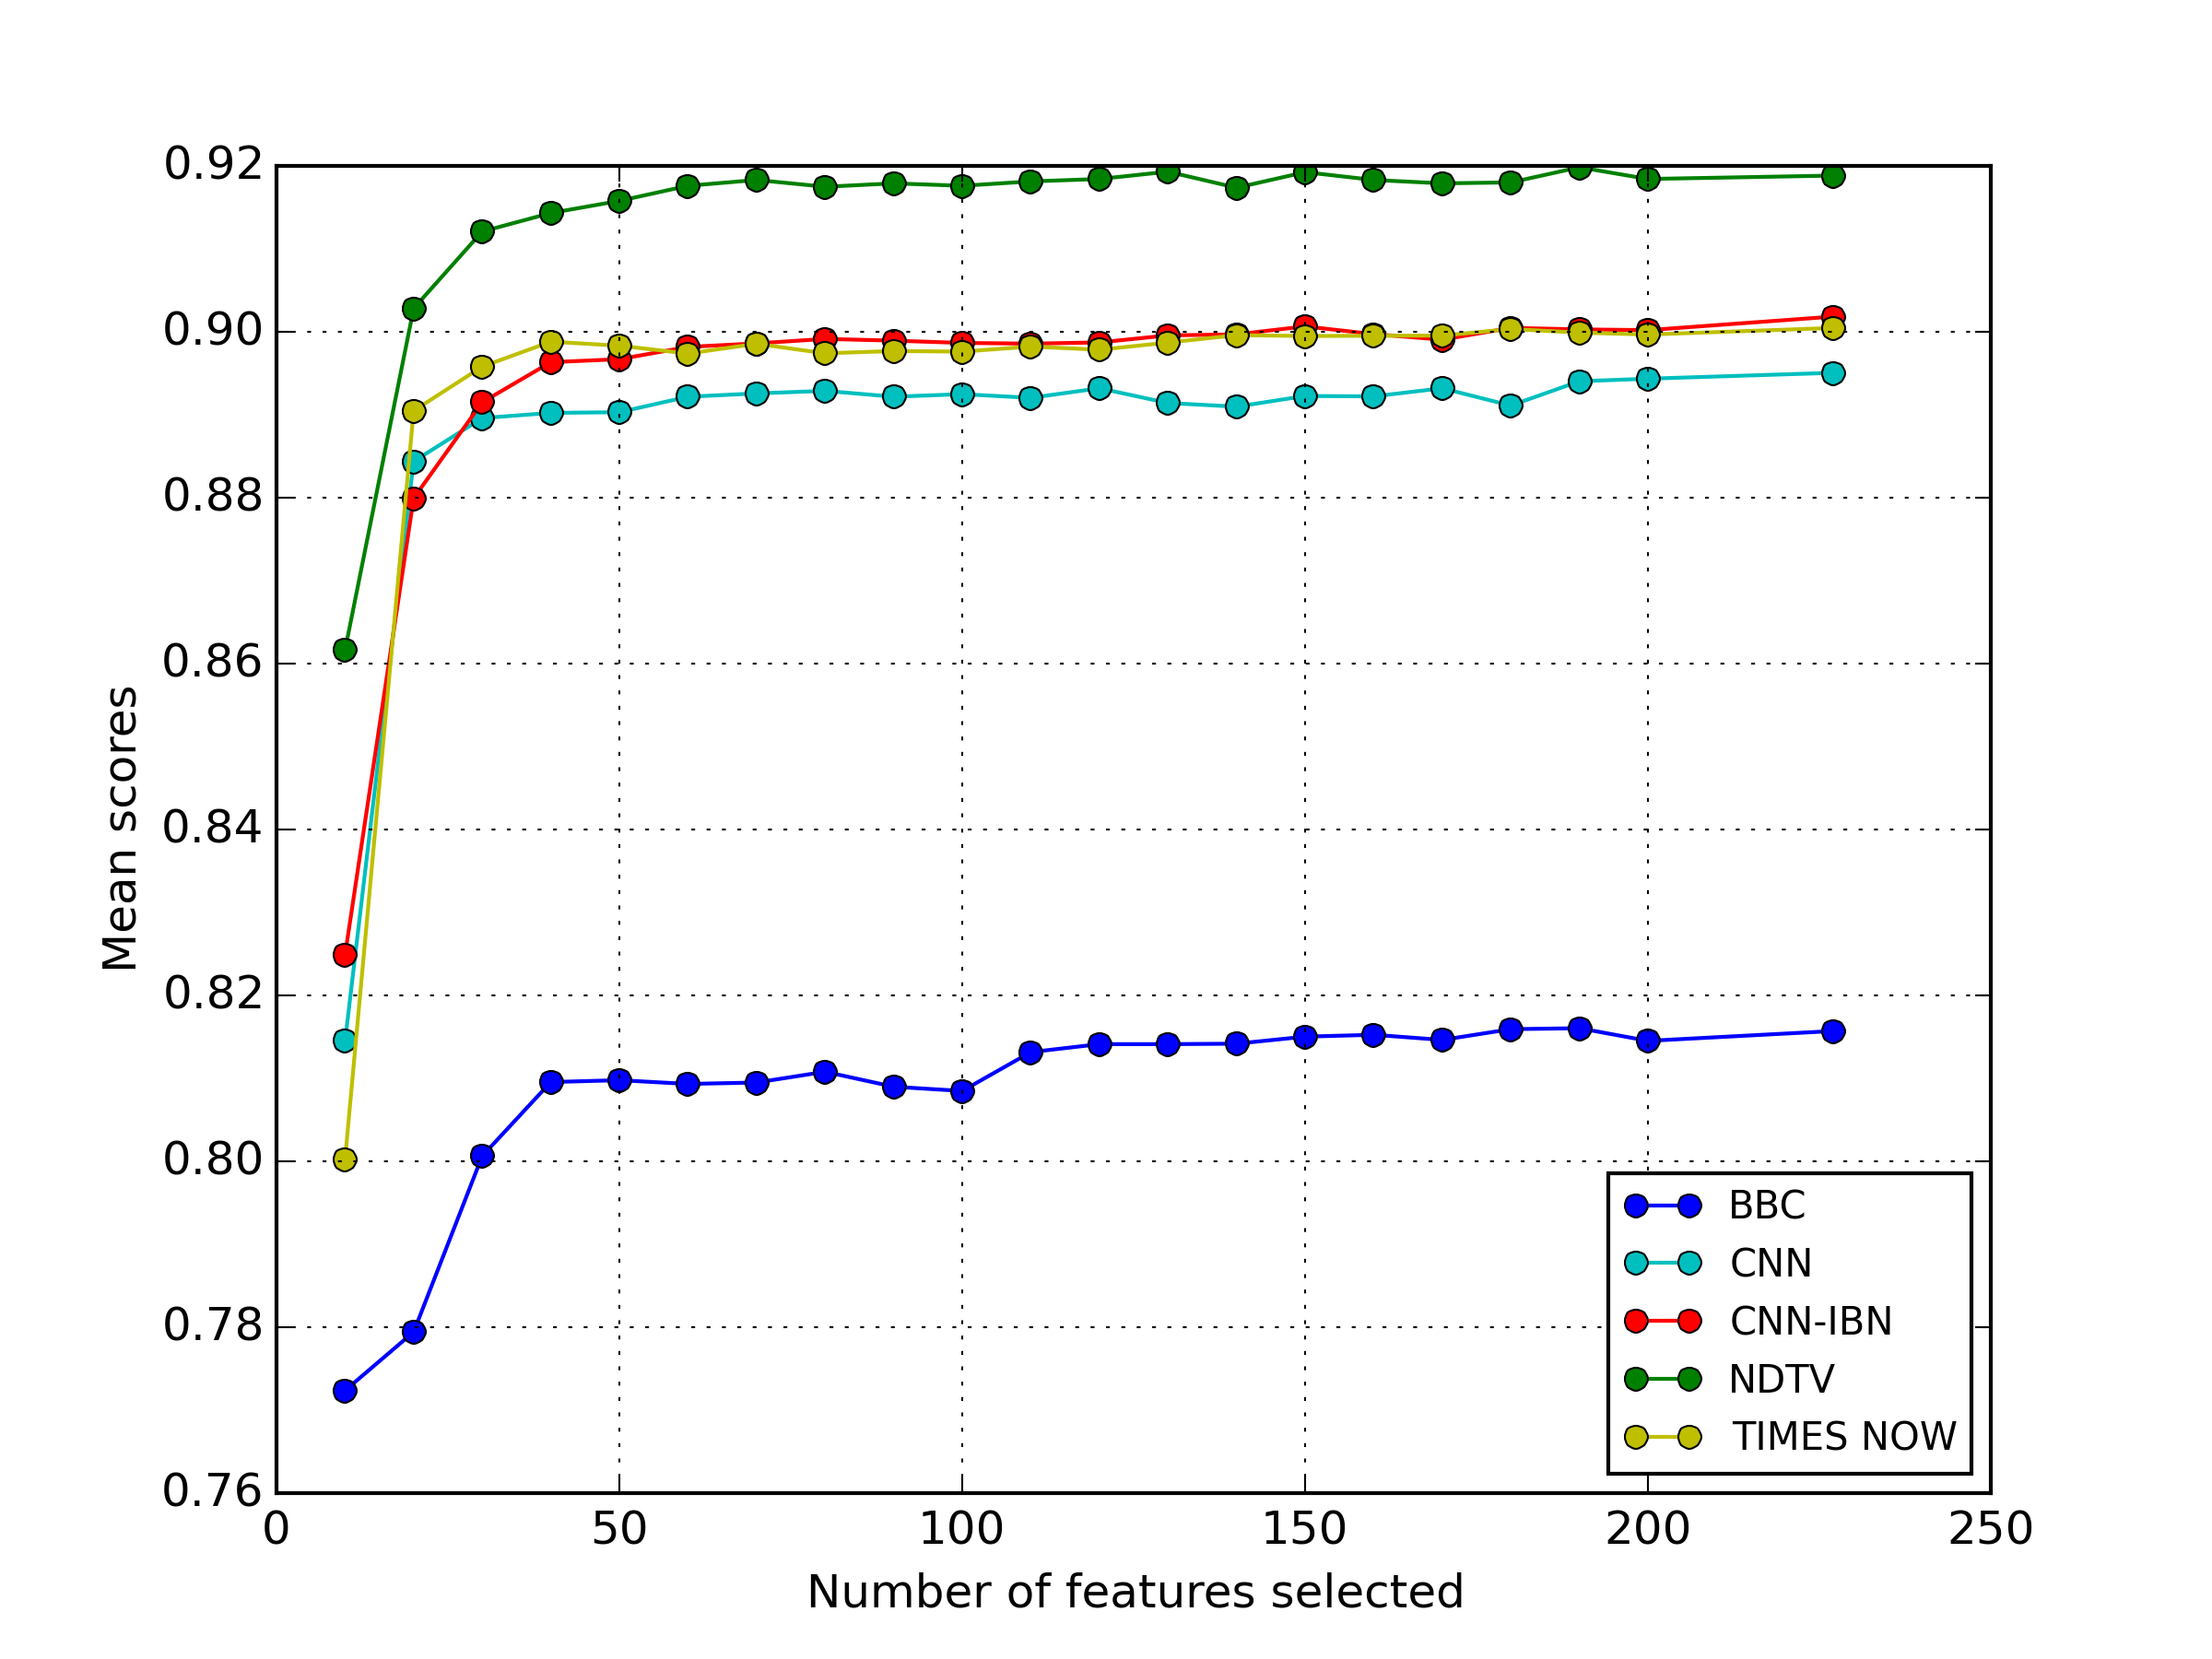
\includegraphics[width=0.5\textwidth]{images/PCA-GTB.png}
    \caption{Gradient tree boosting scores with PCA}
    \label{fig:gtb_pca_scores}
\end{figure} 
 
 \begin{figure}[h!]
    \centering
    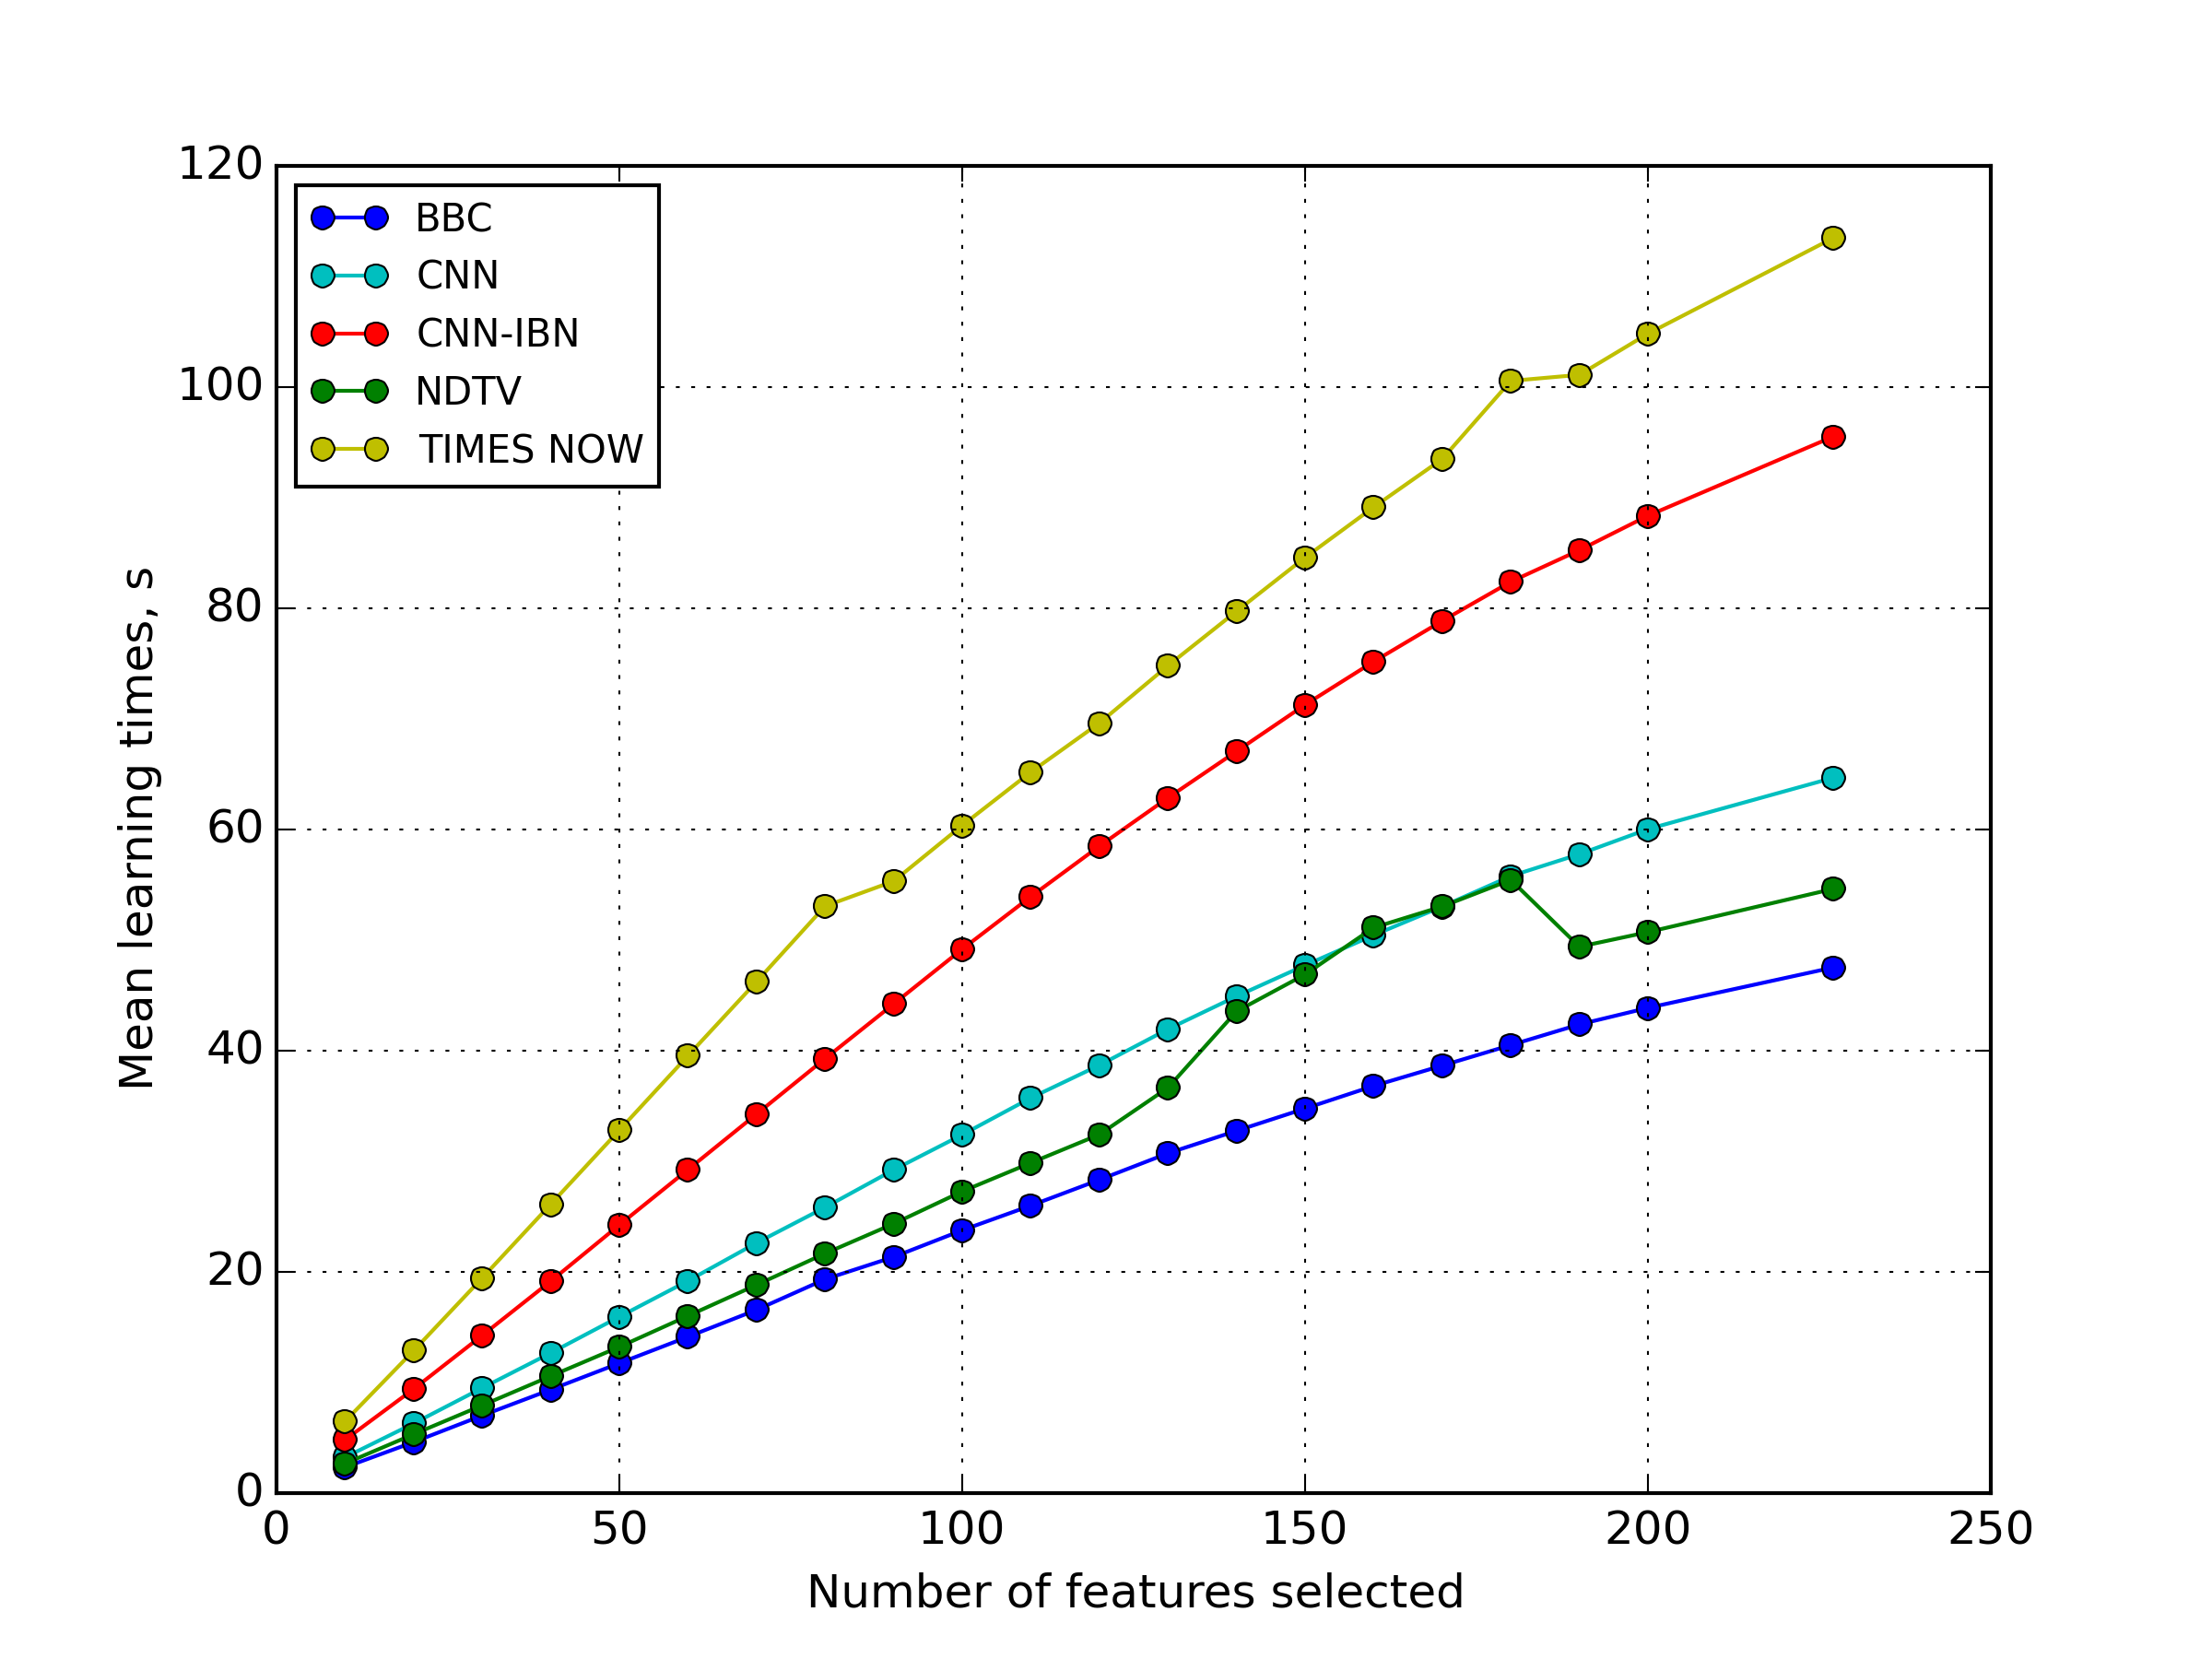
\includegraphics[width=0.5\textwidth]{images/PCA-GTBTime.png}
    \caption{Gradient tree boosting learning times with PCA}
    \label{fig:gtb_pca_times}
\end{figure}

\subsection{Отбор признаков с помощью ансамблей деревьев решений}
Идея о том, что с помощью случайного леса можно для каждого признака можно оценить его важность была высказана в статье Бреймана \cite{breiman}}.
\par
Первые шаг в оценке важности переменной в тренировочной выборке --- обучение случайного леса на этих данных. Во время процесса построения модели для каждого элемента тренировочного набора вычисляется out-of-bag-ошибка.
OOB error --- это доля примеров обучающей выборки, неправильно классифицируемых лесом, если не учитывать голоса деревьев на примерах, входящих в их собственную бутстрап подвыборку.
Для того, чтобы оценить важность j-го признака после тренировки, значения j-го параметра перемешиваются для всех записей тренировочного набора и out-of-bag-ошибка считается снова. Важность признака оценивается путем усреднения по всем деревьям разности показателей out-of-bag-ошибок до и после перемешивания значений. При этом значения таких ошибок нормализуются на среднеквадратическое отклонение разностей.
После этого осуществляется отсечение признаков с низким весом по заданному порогу. Можно также выбирать k самых важных признаков, что и будет делаться далее.
\subsubsection*{Результаты отбора признаков с помощью случайного леса}
В качестве классификатора для оценки важности признаков выступает случайный лес из 60-ти деревьев. Схема экспериментов такая же, как с PCA. Из-за недостатка времени эксперименты не были проведены полностью (результаты методов SVM и GTB получены для двух каналов), однако их достаточно, чтобы сказать, что отбор по важности проявил себя не хуже, чем PCA.
\par
На некоторых каналах метода \(k\) ближайших соседей показывает нехарактерно высокое для него качество классификации при маленьком количестве признаков (рис. \ref{fig:knn_rfs_scores}). Скорее всего, это случайность, так как при дальнейшем увеличении количества признаков качество классификации резко падает и стабилизируется на значении, которое было до редукции размерности.
\begin{figure}[h!]
    \centering
    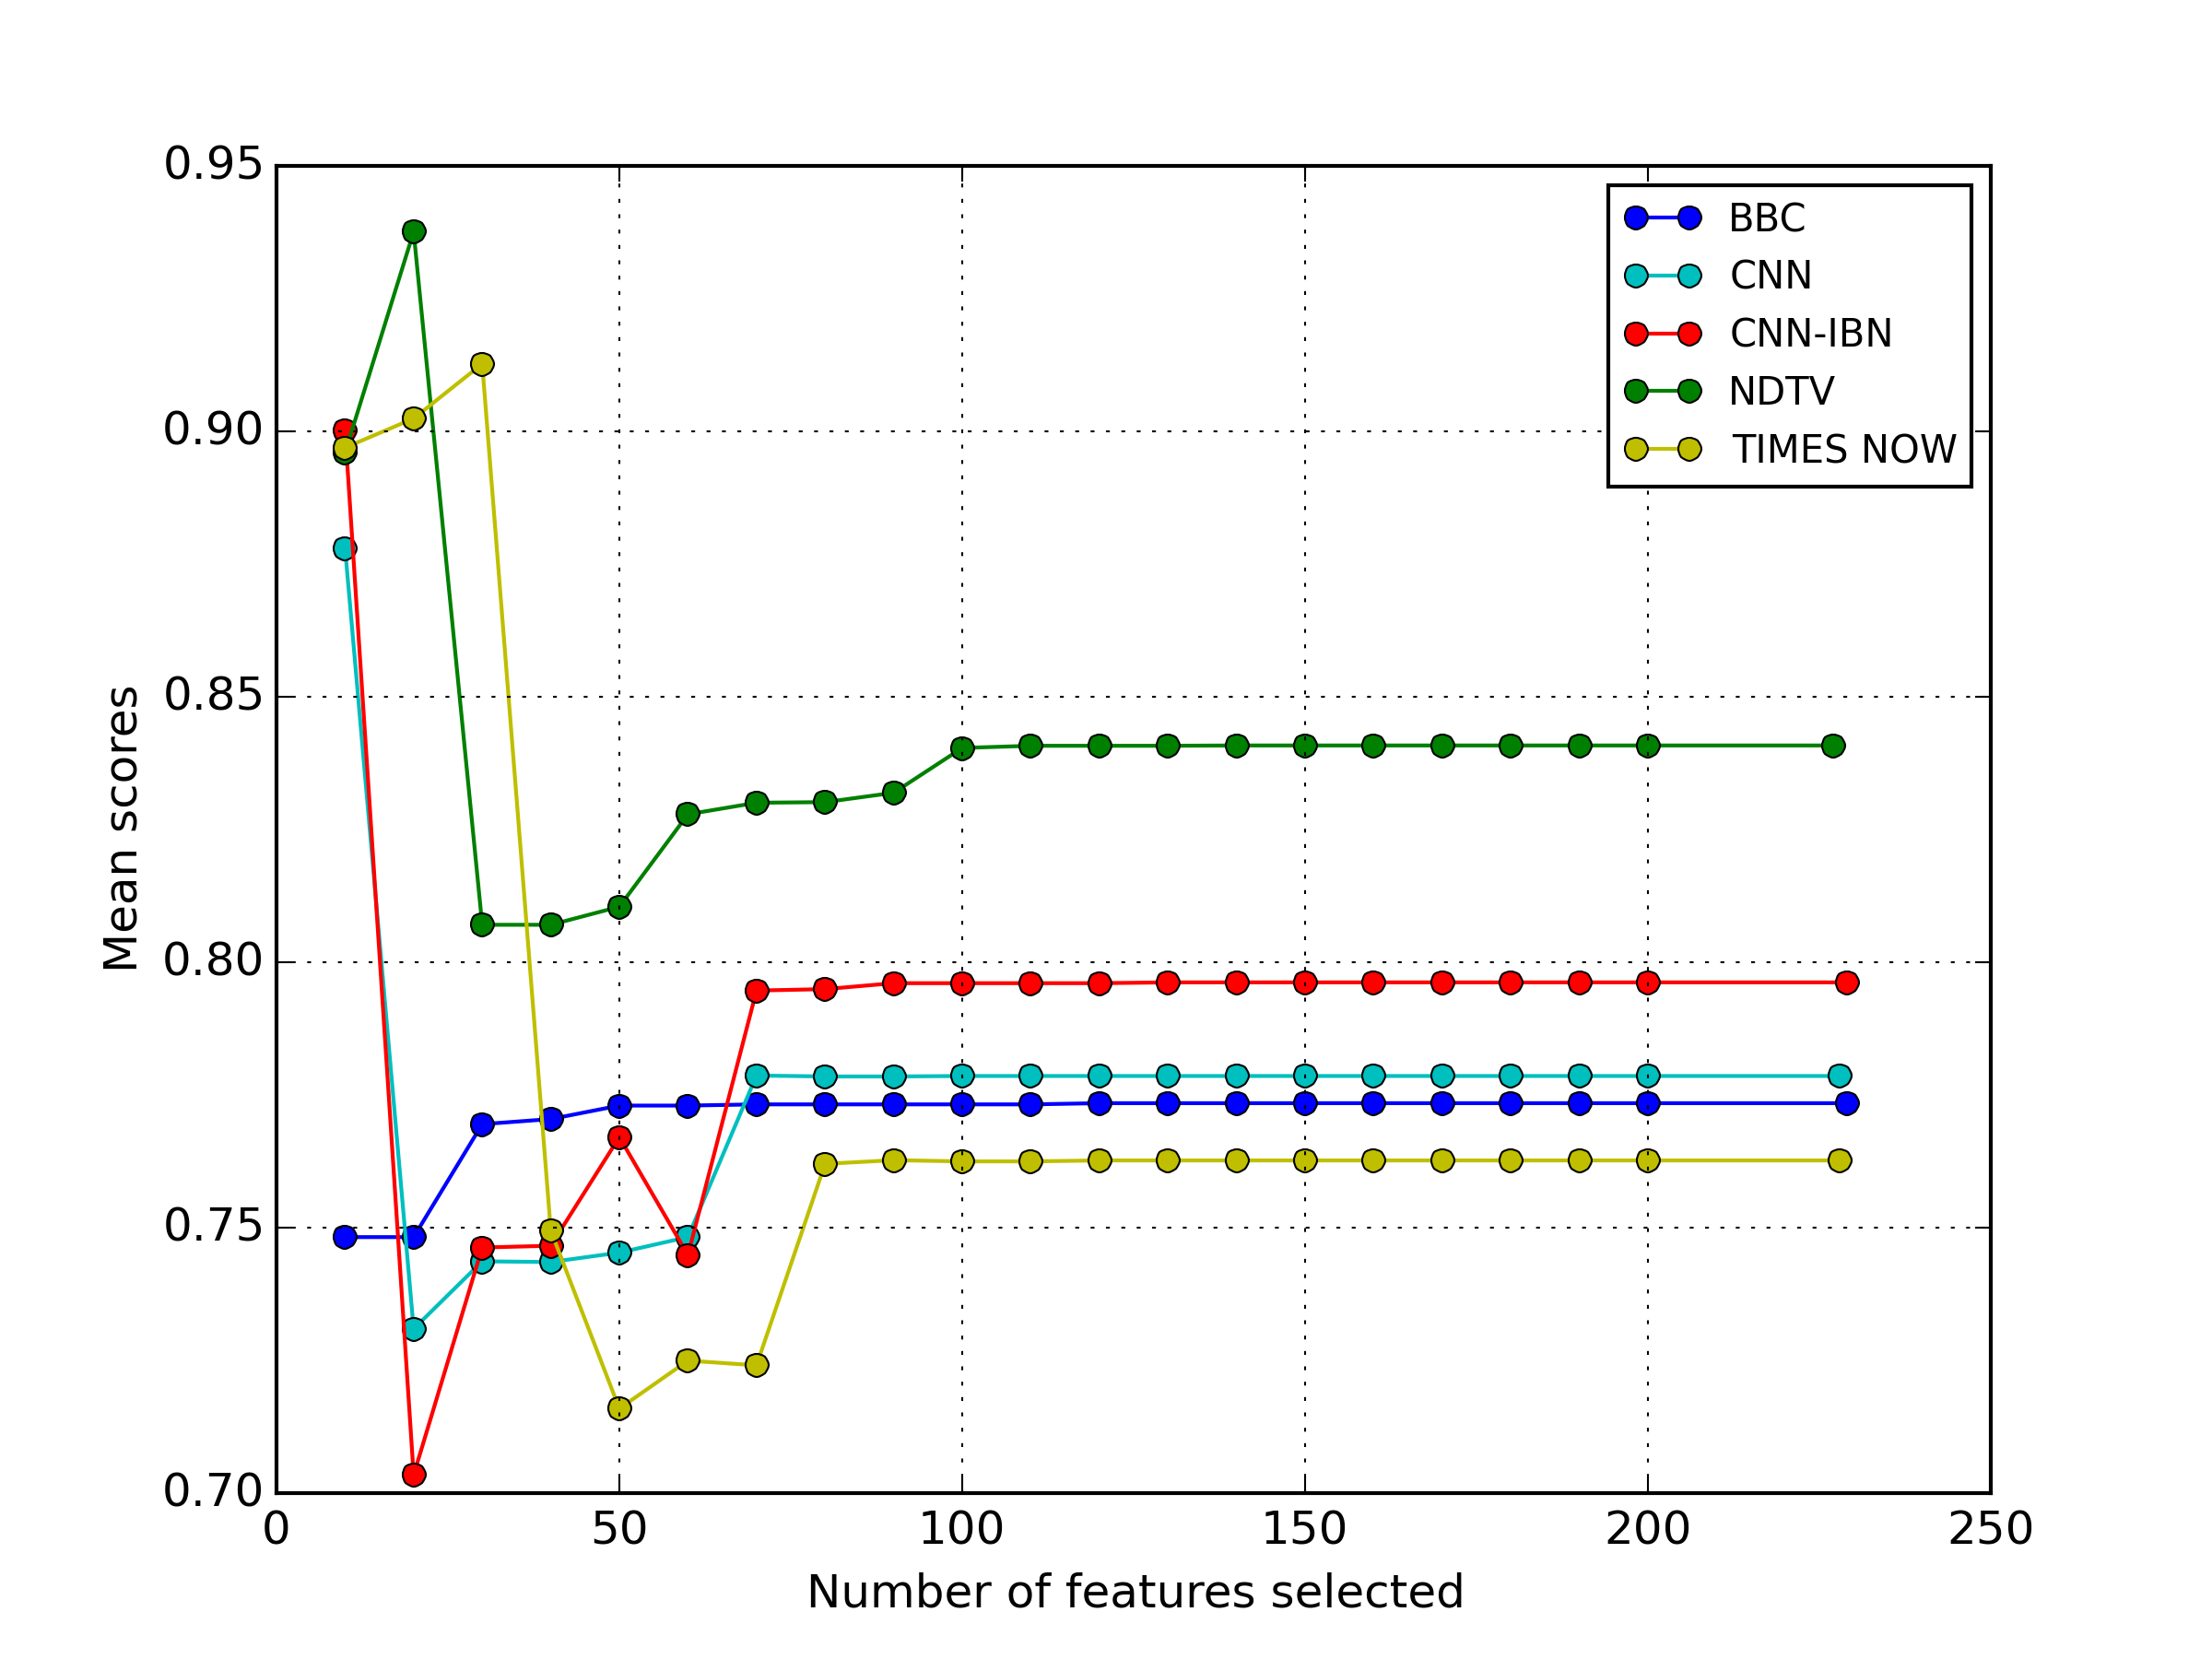
\includegraphics[width=0.5\textwidth]{images/RFS-kNN.png}
    \caption{\(k\)NN scores with RFS}
    \label{fig:knn_rfs_scores}
\end{figure} 
\begin{figure}[h!]
    \centering
    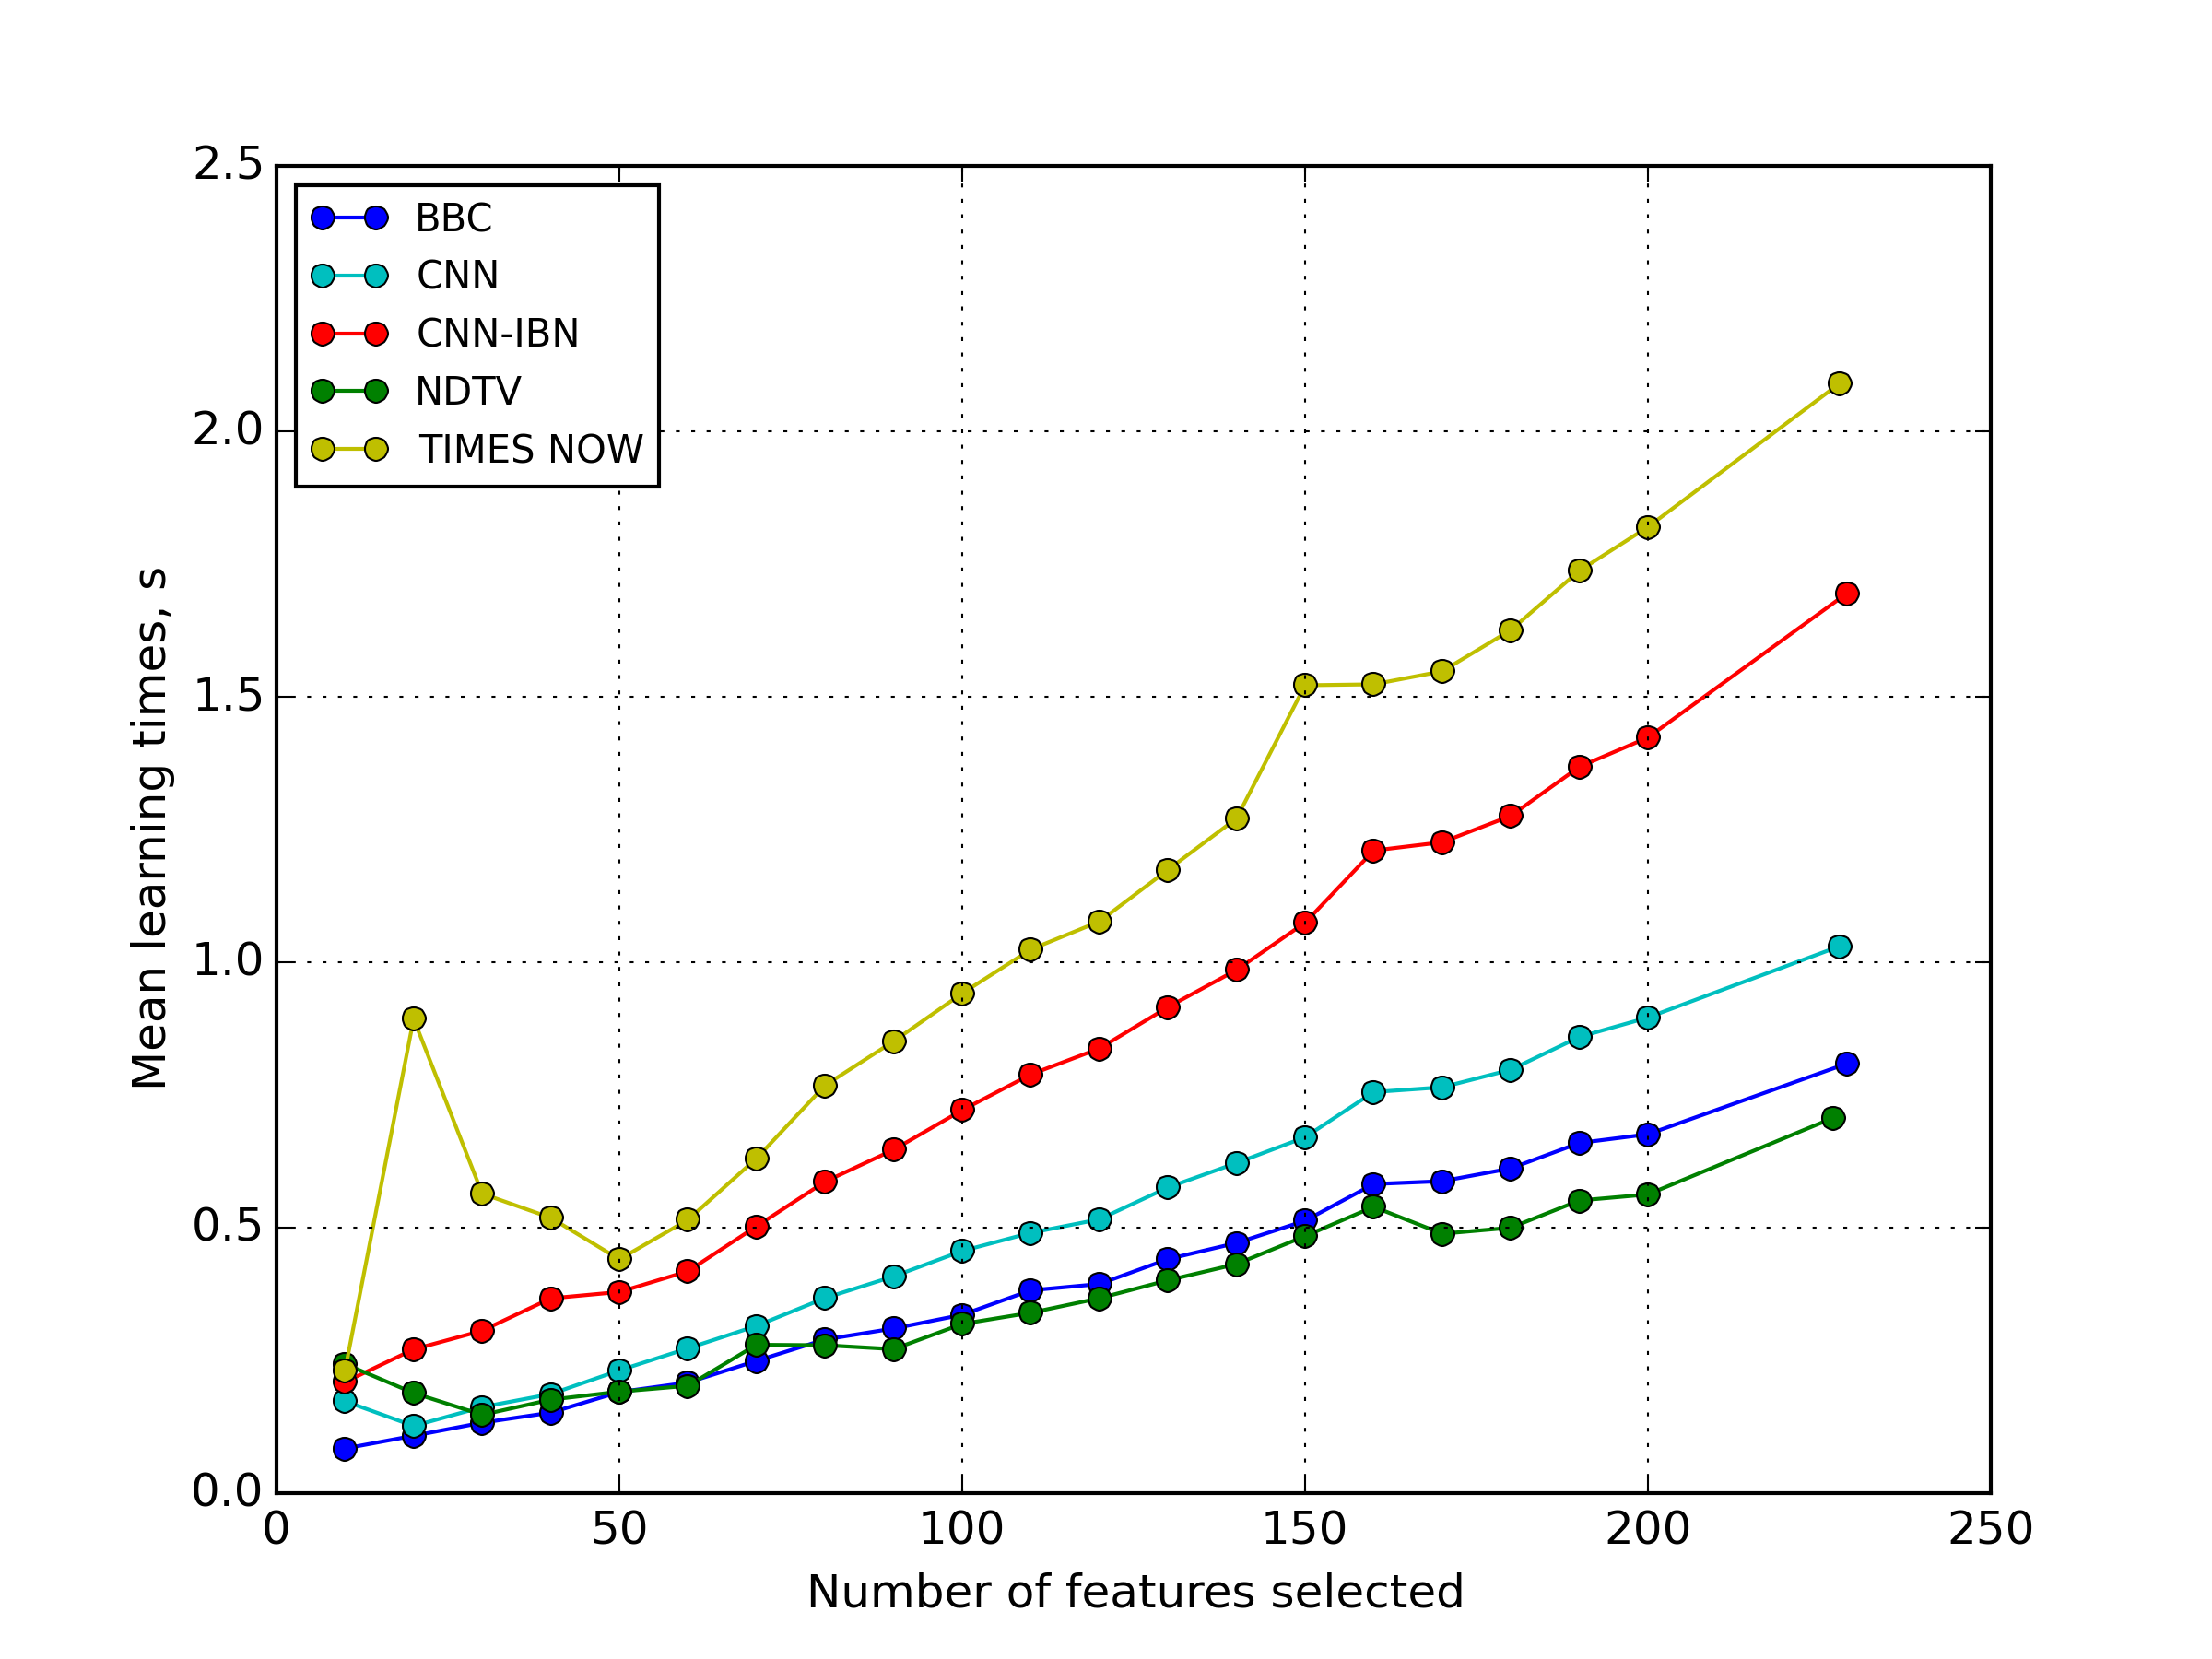
\includegraphics[width=0.5\textwidth]{images/RFS-kNNTime.png}
    \caption{\(k\)NN learning times with RFS}
    \label{fig:knn_rfs_times}
\end{figure} 

\par
Как и в случае с PCA, качество классификации линейного дискриминантного анализа монотонно ухудшается при снижении размерности данных (рис. \ref{fig:lda_rfs_scores}).

\begin{figure}[h!]
    \centering
    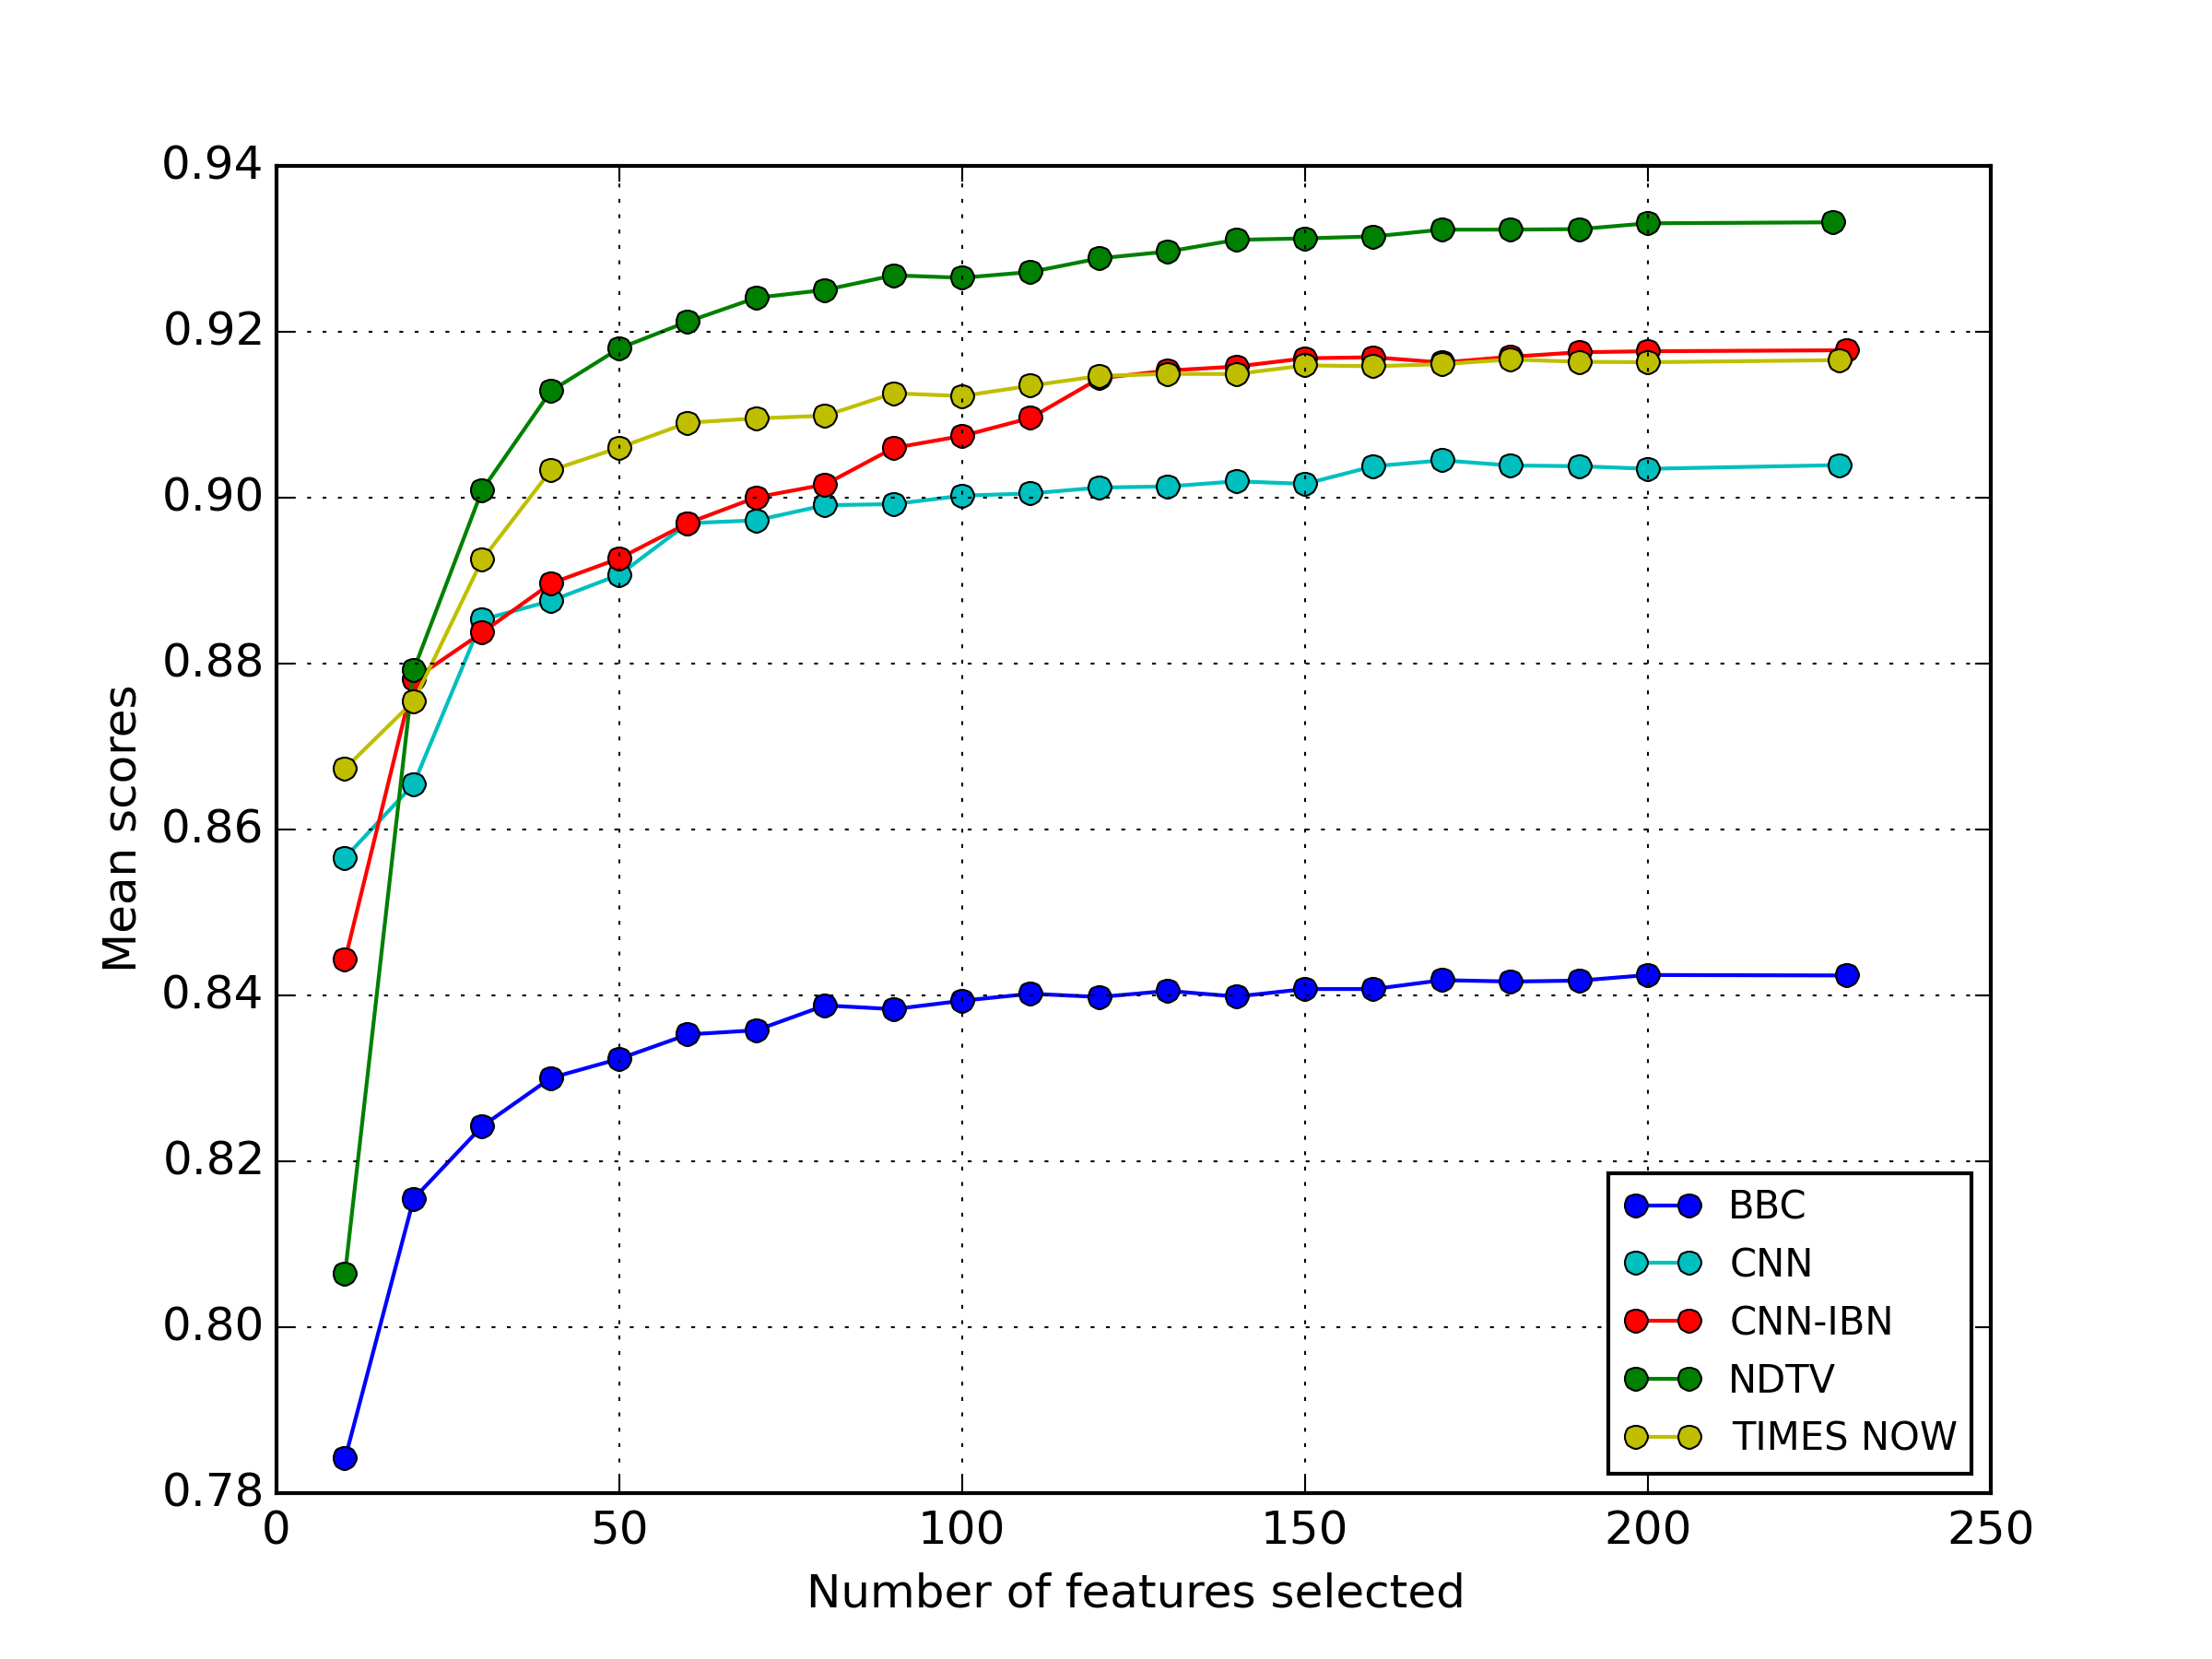
\includegraphics[width=0.5\textwidth]{images/RFS-LDA.png}
    \caption{LDA scores with RFS}
    \label{fig:lda_rfs_scores}
\end{figure} 
\begin{figure}[h!]
    \centering
    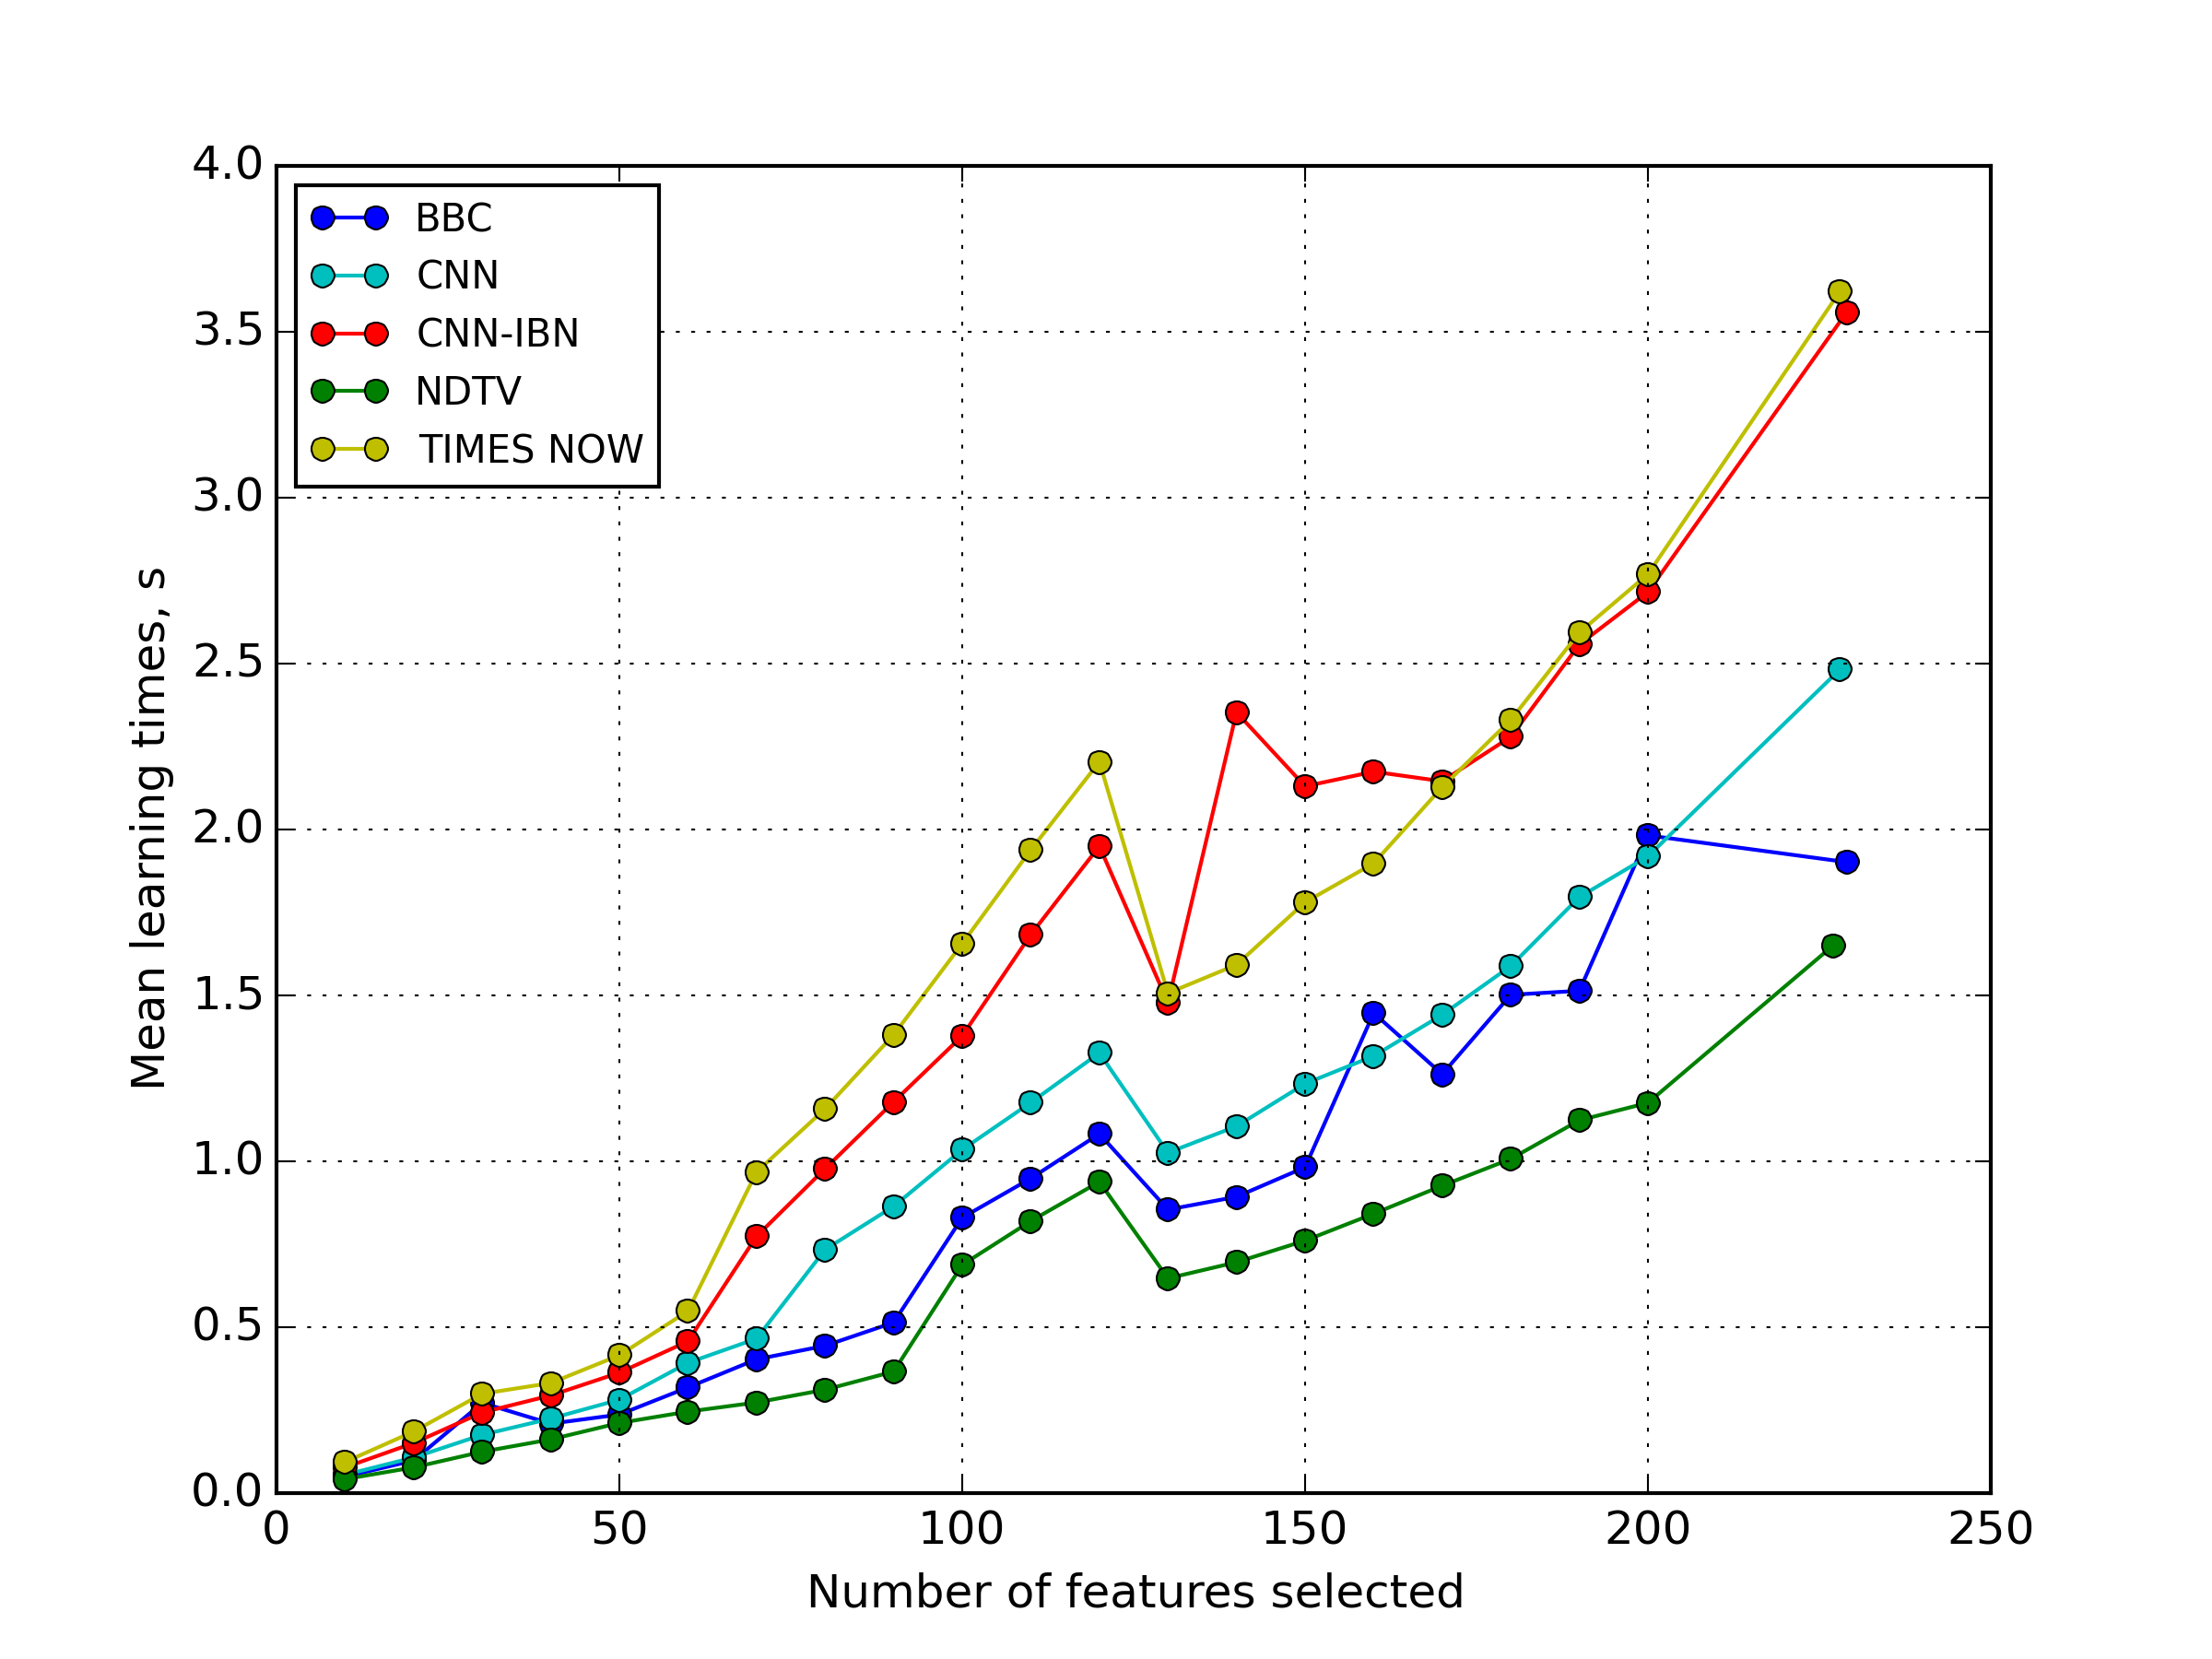
\includegraphics[width=0.5\textwidth]{images/RFS-LDATime.png}
    \caption{LDA learning times with RFS}
    \label{fig:lda_rfs_times}
\end{figure} 
\par
Результаты, полученные на части данных показывают, что качество классификации SVM можно повысить путём отбора признаков с момощью случайного леса. Оптимальное значение количества признаков --- 100 или 110 в зависимости от данных.

\begin{figure}[h!]
    \centering
    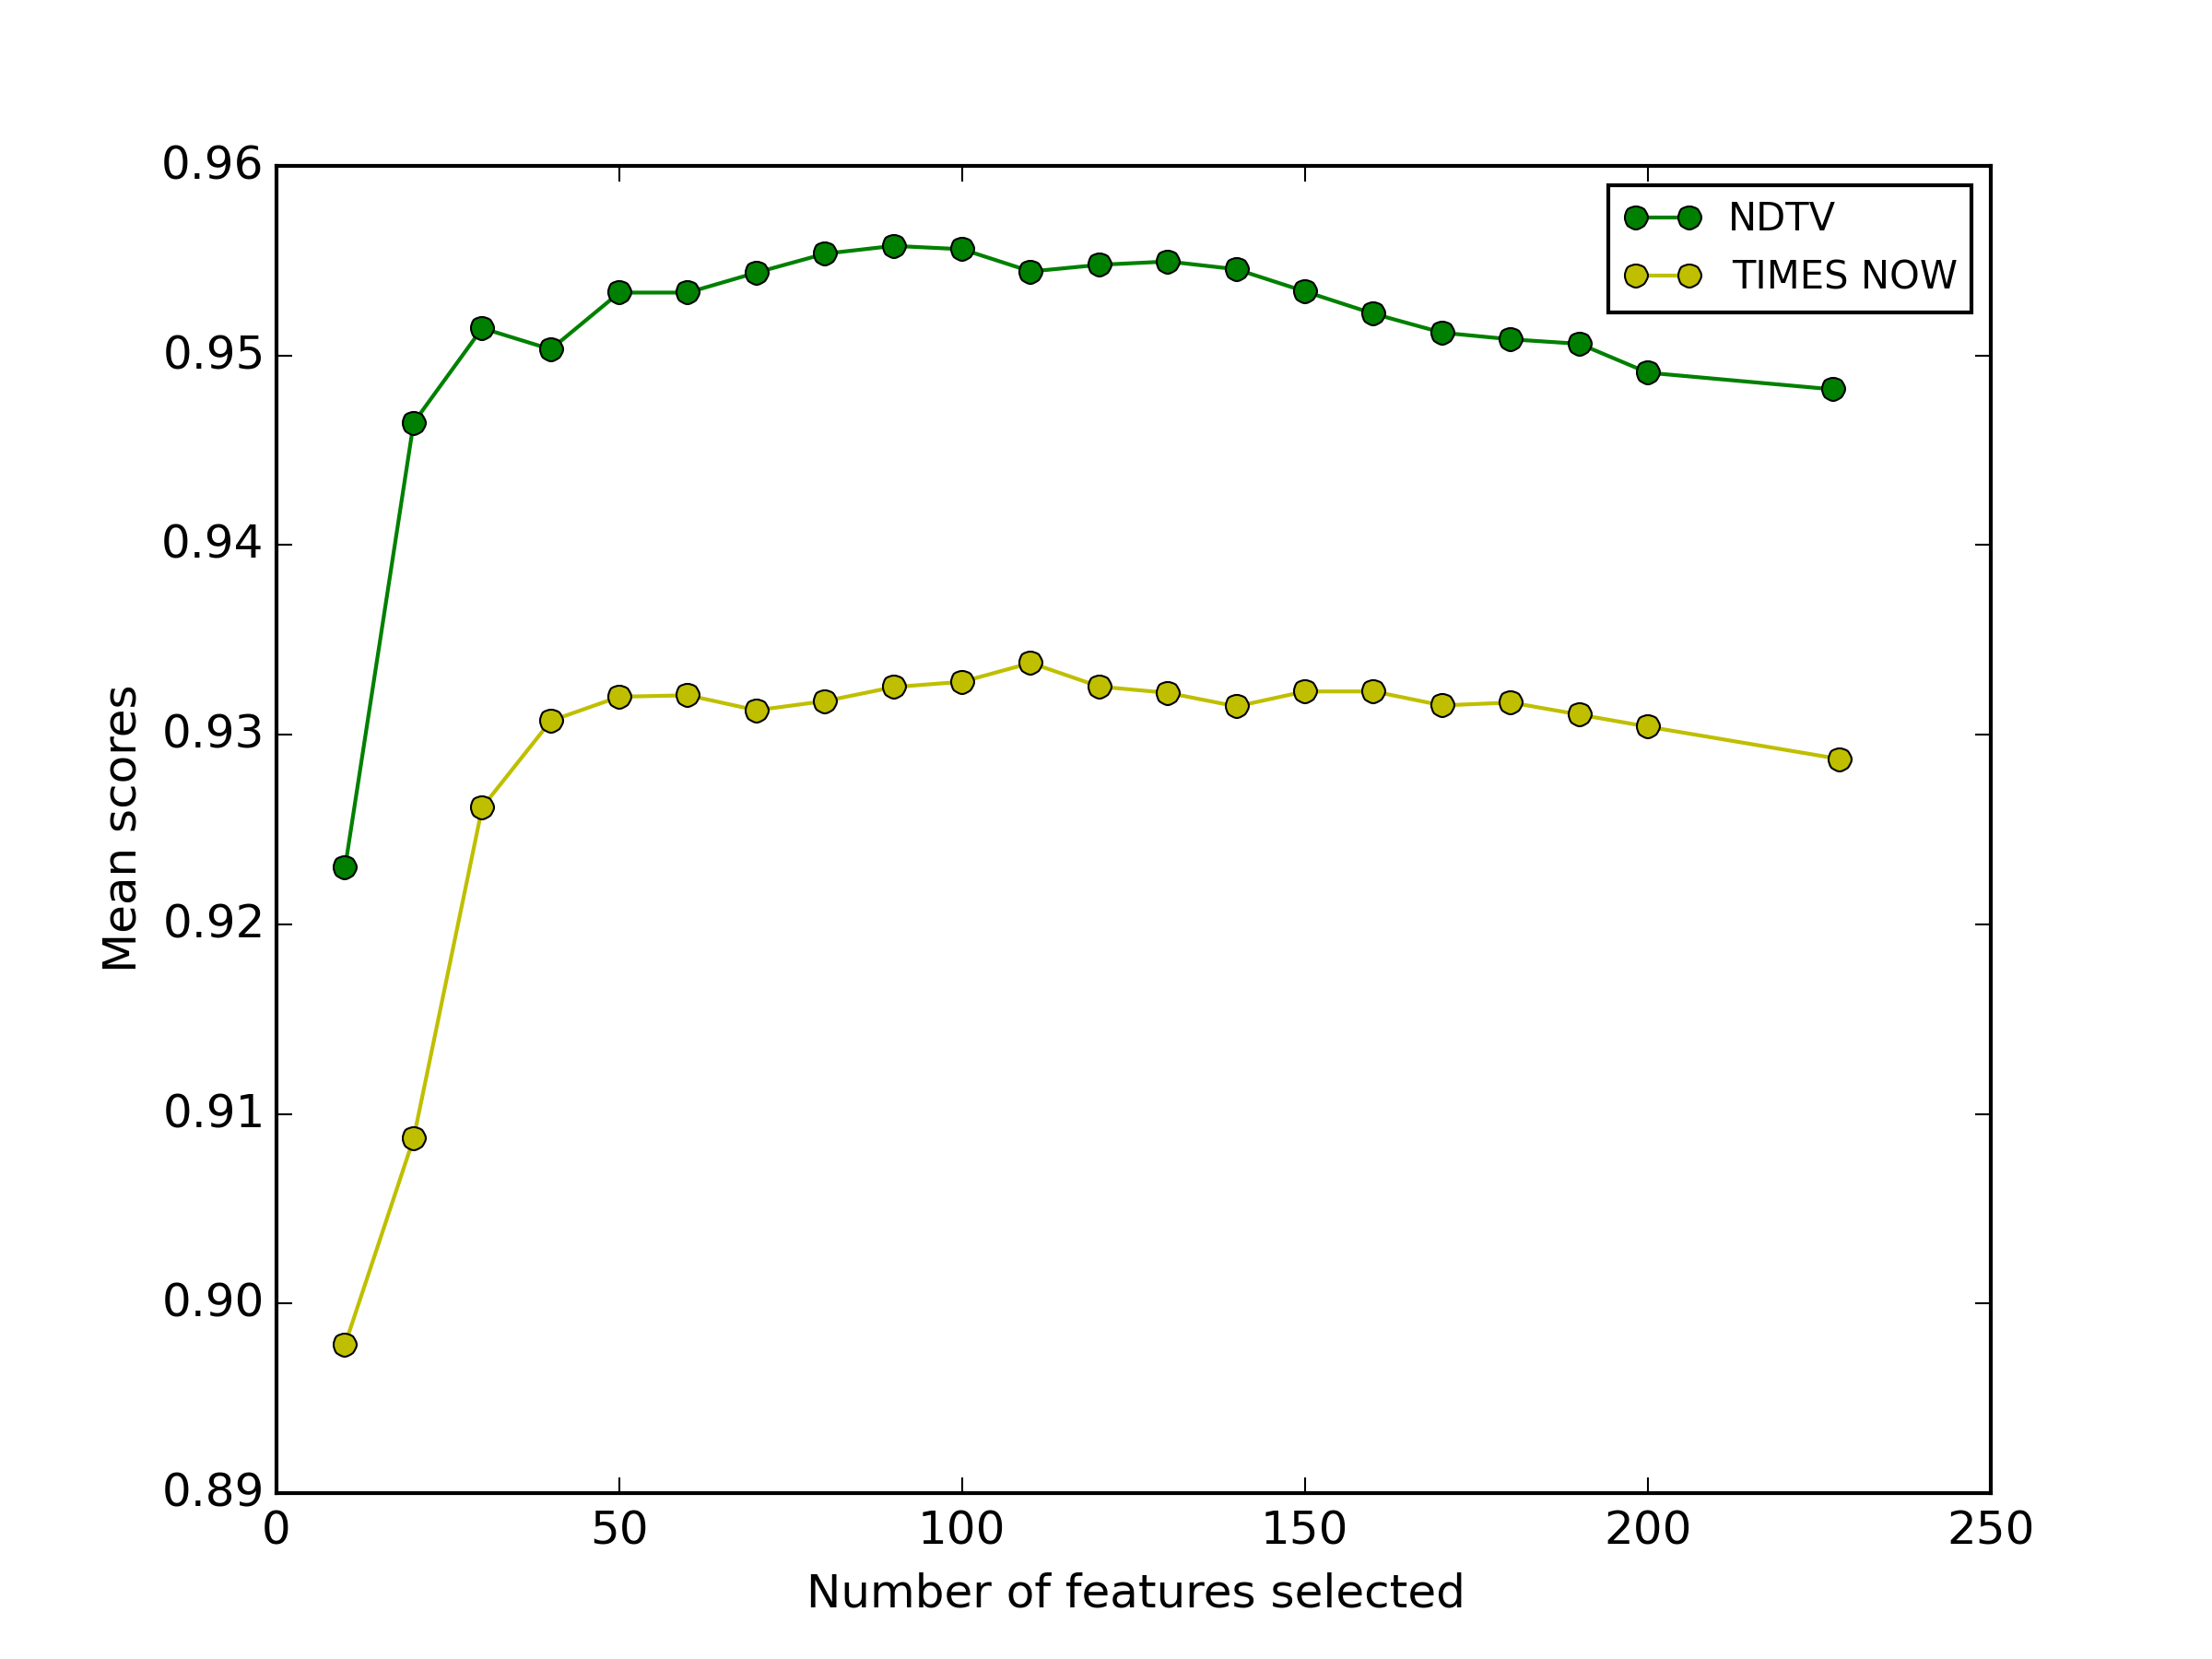
\includegraphics[width=0.5\textwidth]{images/RFS-SVM.png}
    \caption{SVM scores with RFS}
    \label{fig:svm_rfs_scores}
\end{figure} 
\begin{figure}[h!]
    \centering
    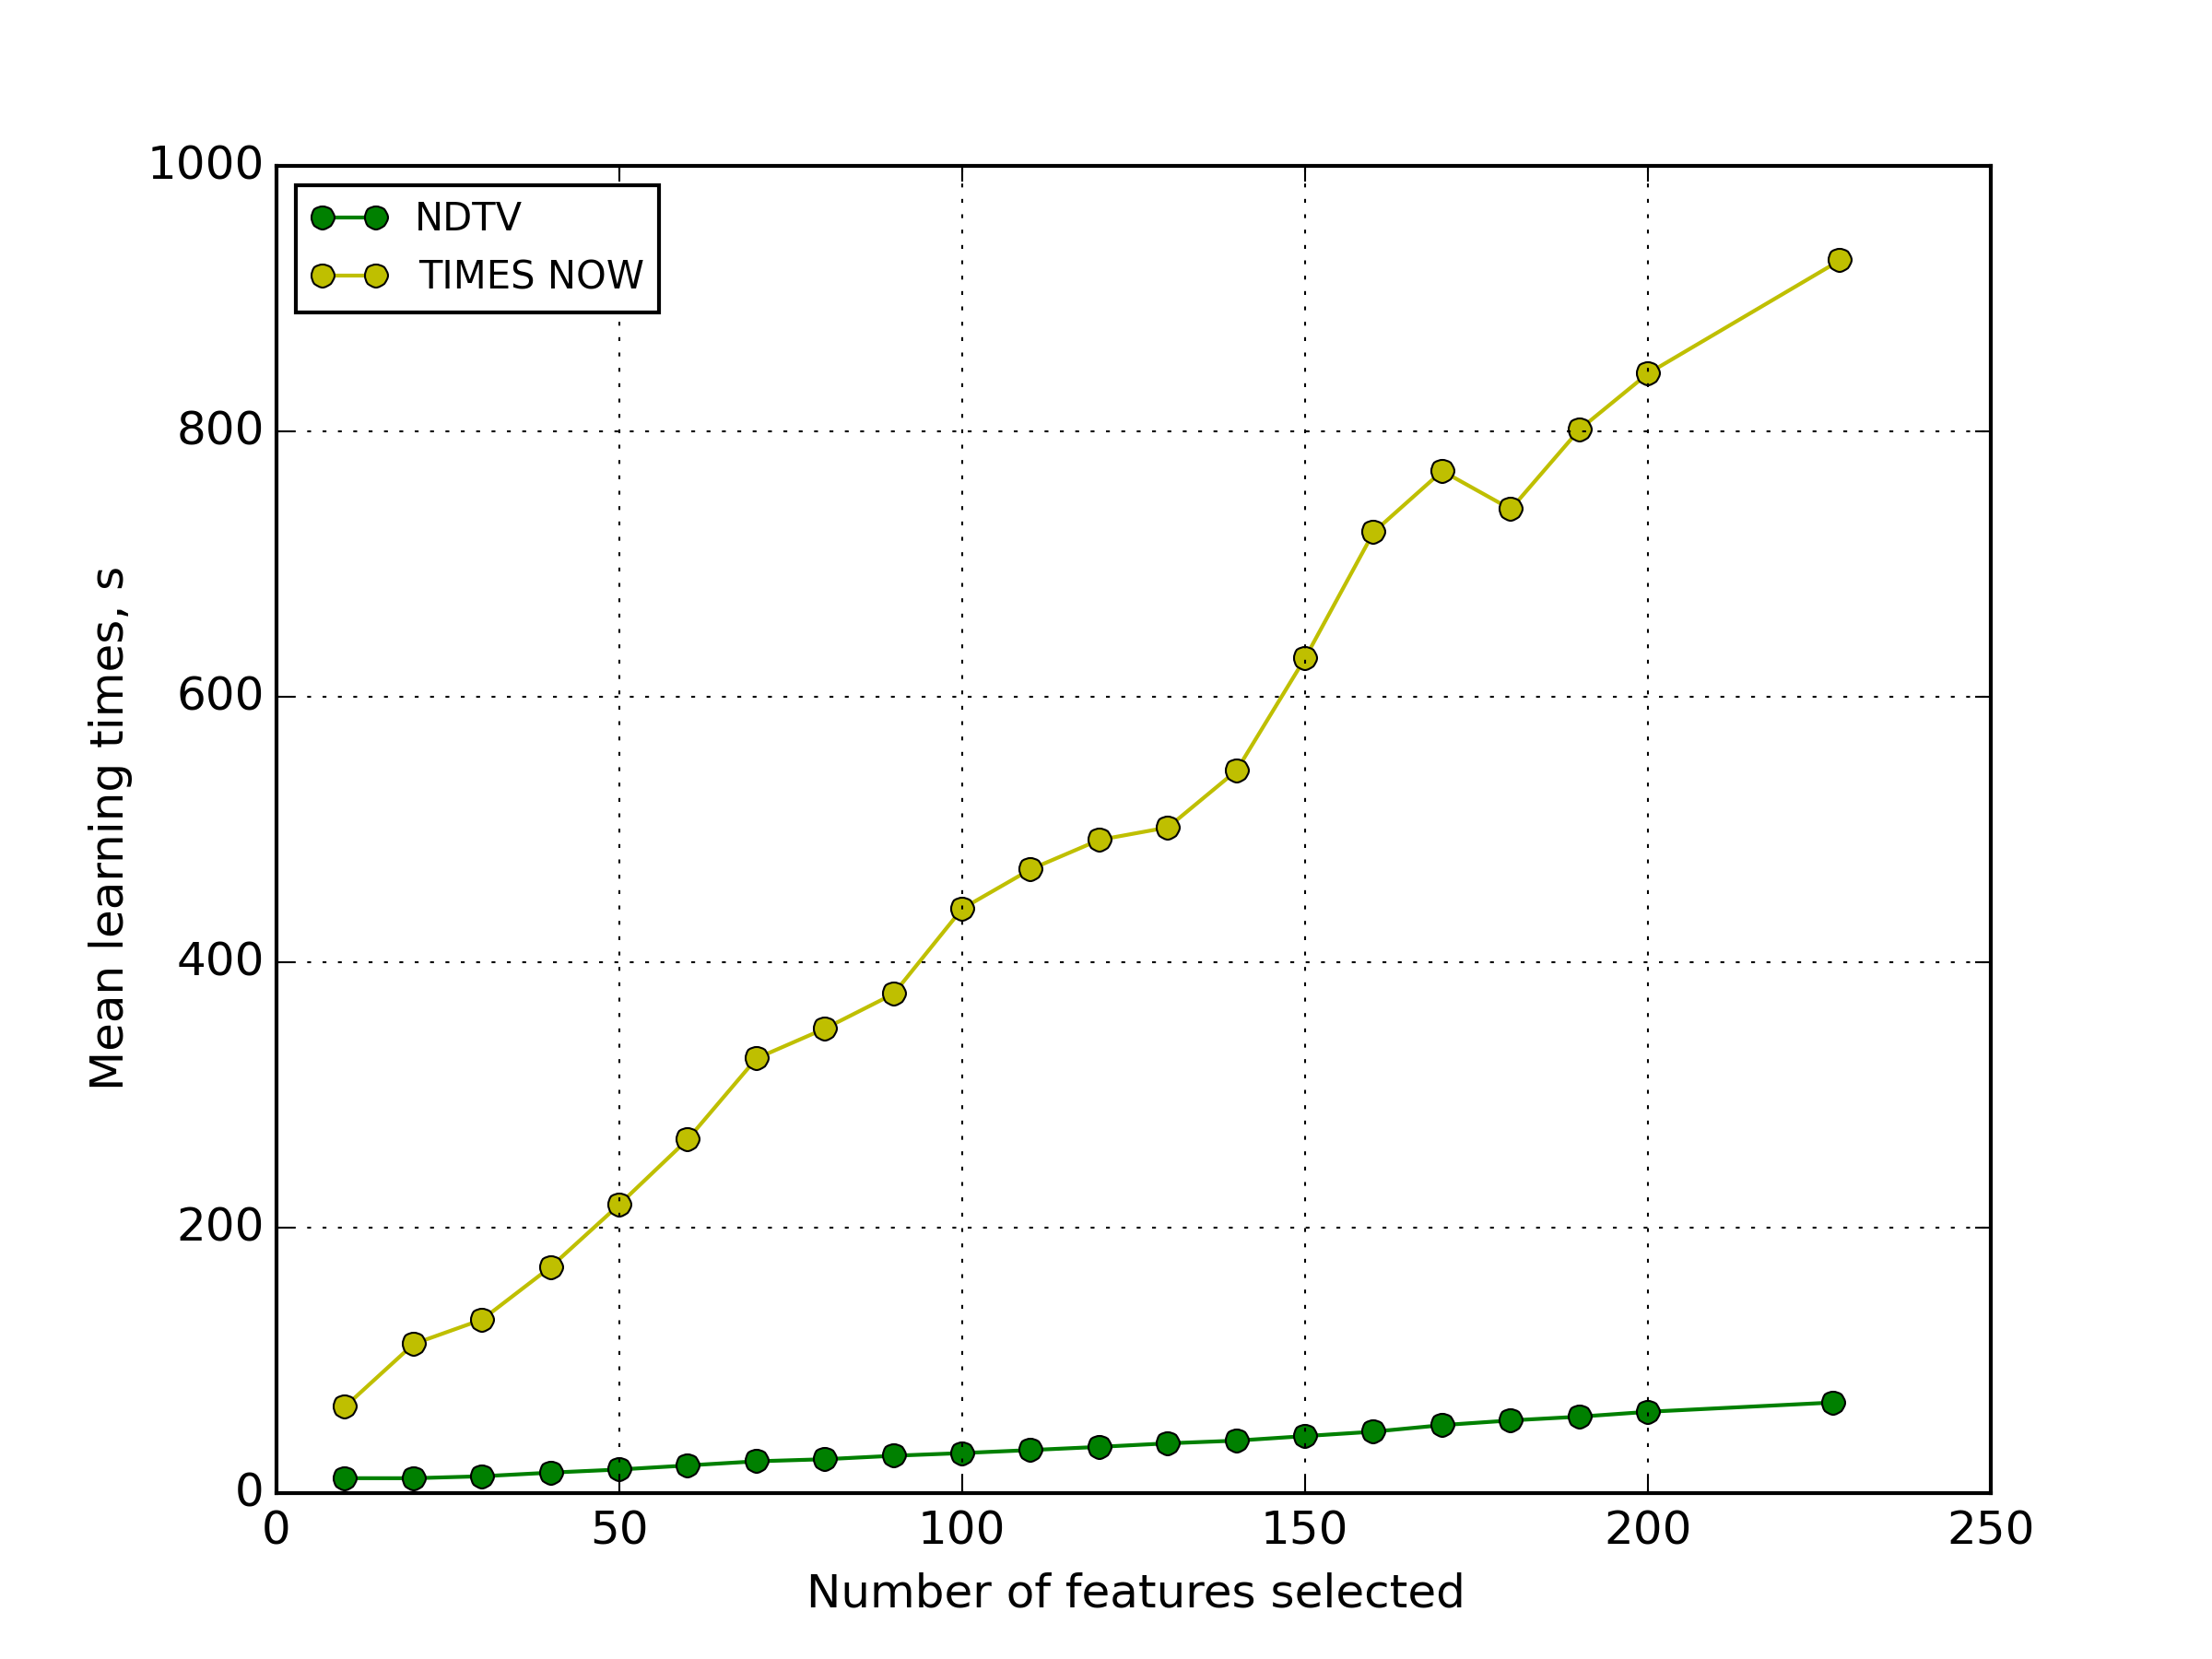
\includegraphics[width=0.5\textwidth]{images/RFS-SVMTime.png}
    \caption{SVM learning times with RFS}
    \label{fig:svm_rfs_times}
\end{figure} 

\par
Отбор признаков практически не влияет на качество классификации случайного леса, поэтому делать это имеет смысл только для уменьшения время тренировки и объёма тренировочных данных.

\begin{figure}[h!]
    \centering
    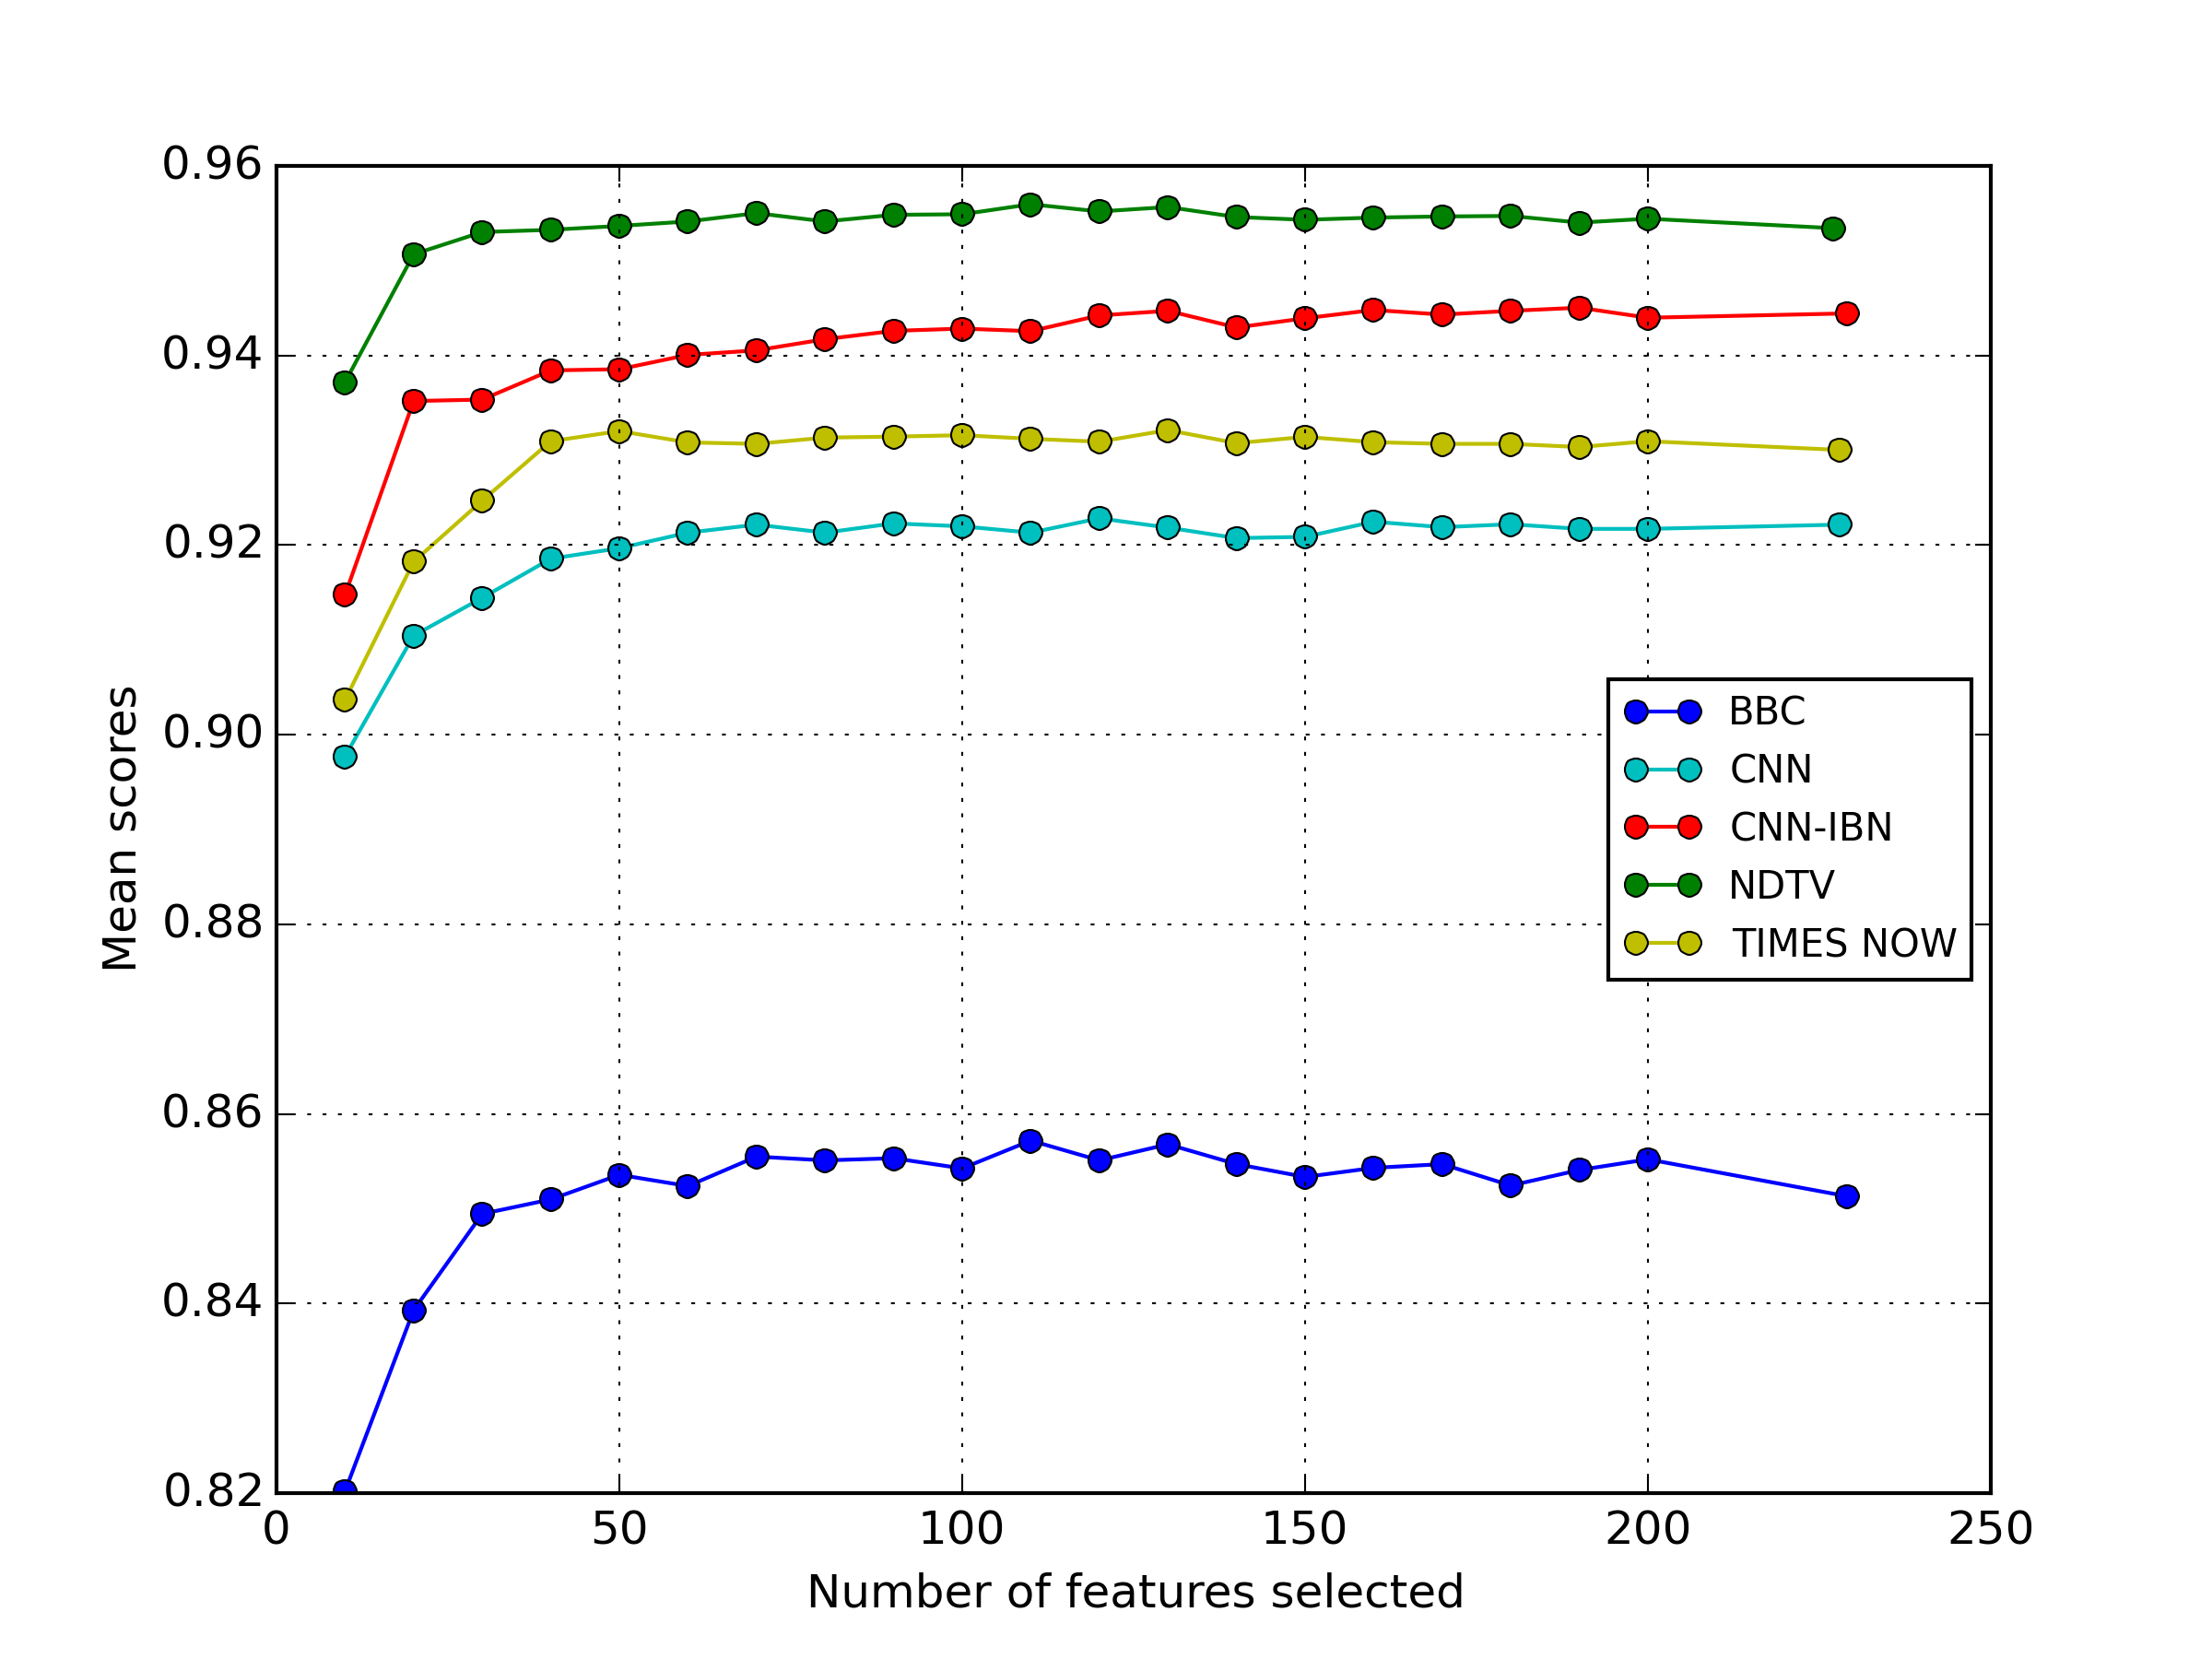
\includegraphics[width=0.5\textwidth]{images/RFS-randforest.png}
    \caption{Random forest scores with RFS}
    \label{fig:randfor_rfs_scores}
\end{figure} 
 
 \begin{figure}[h!]
    \centering
    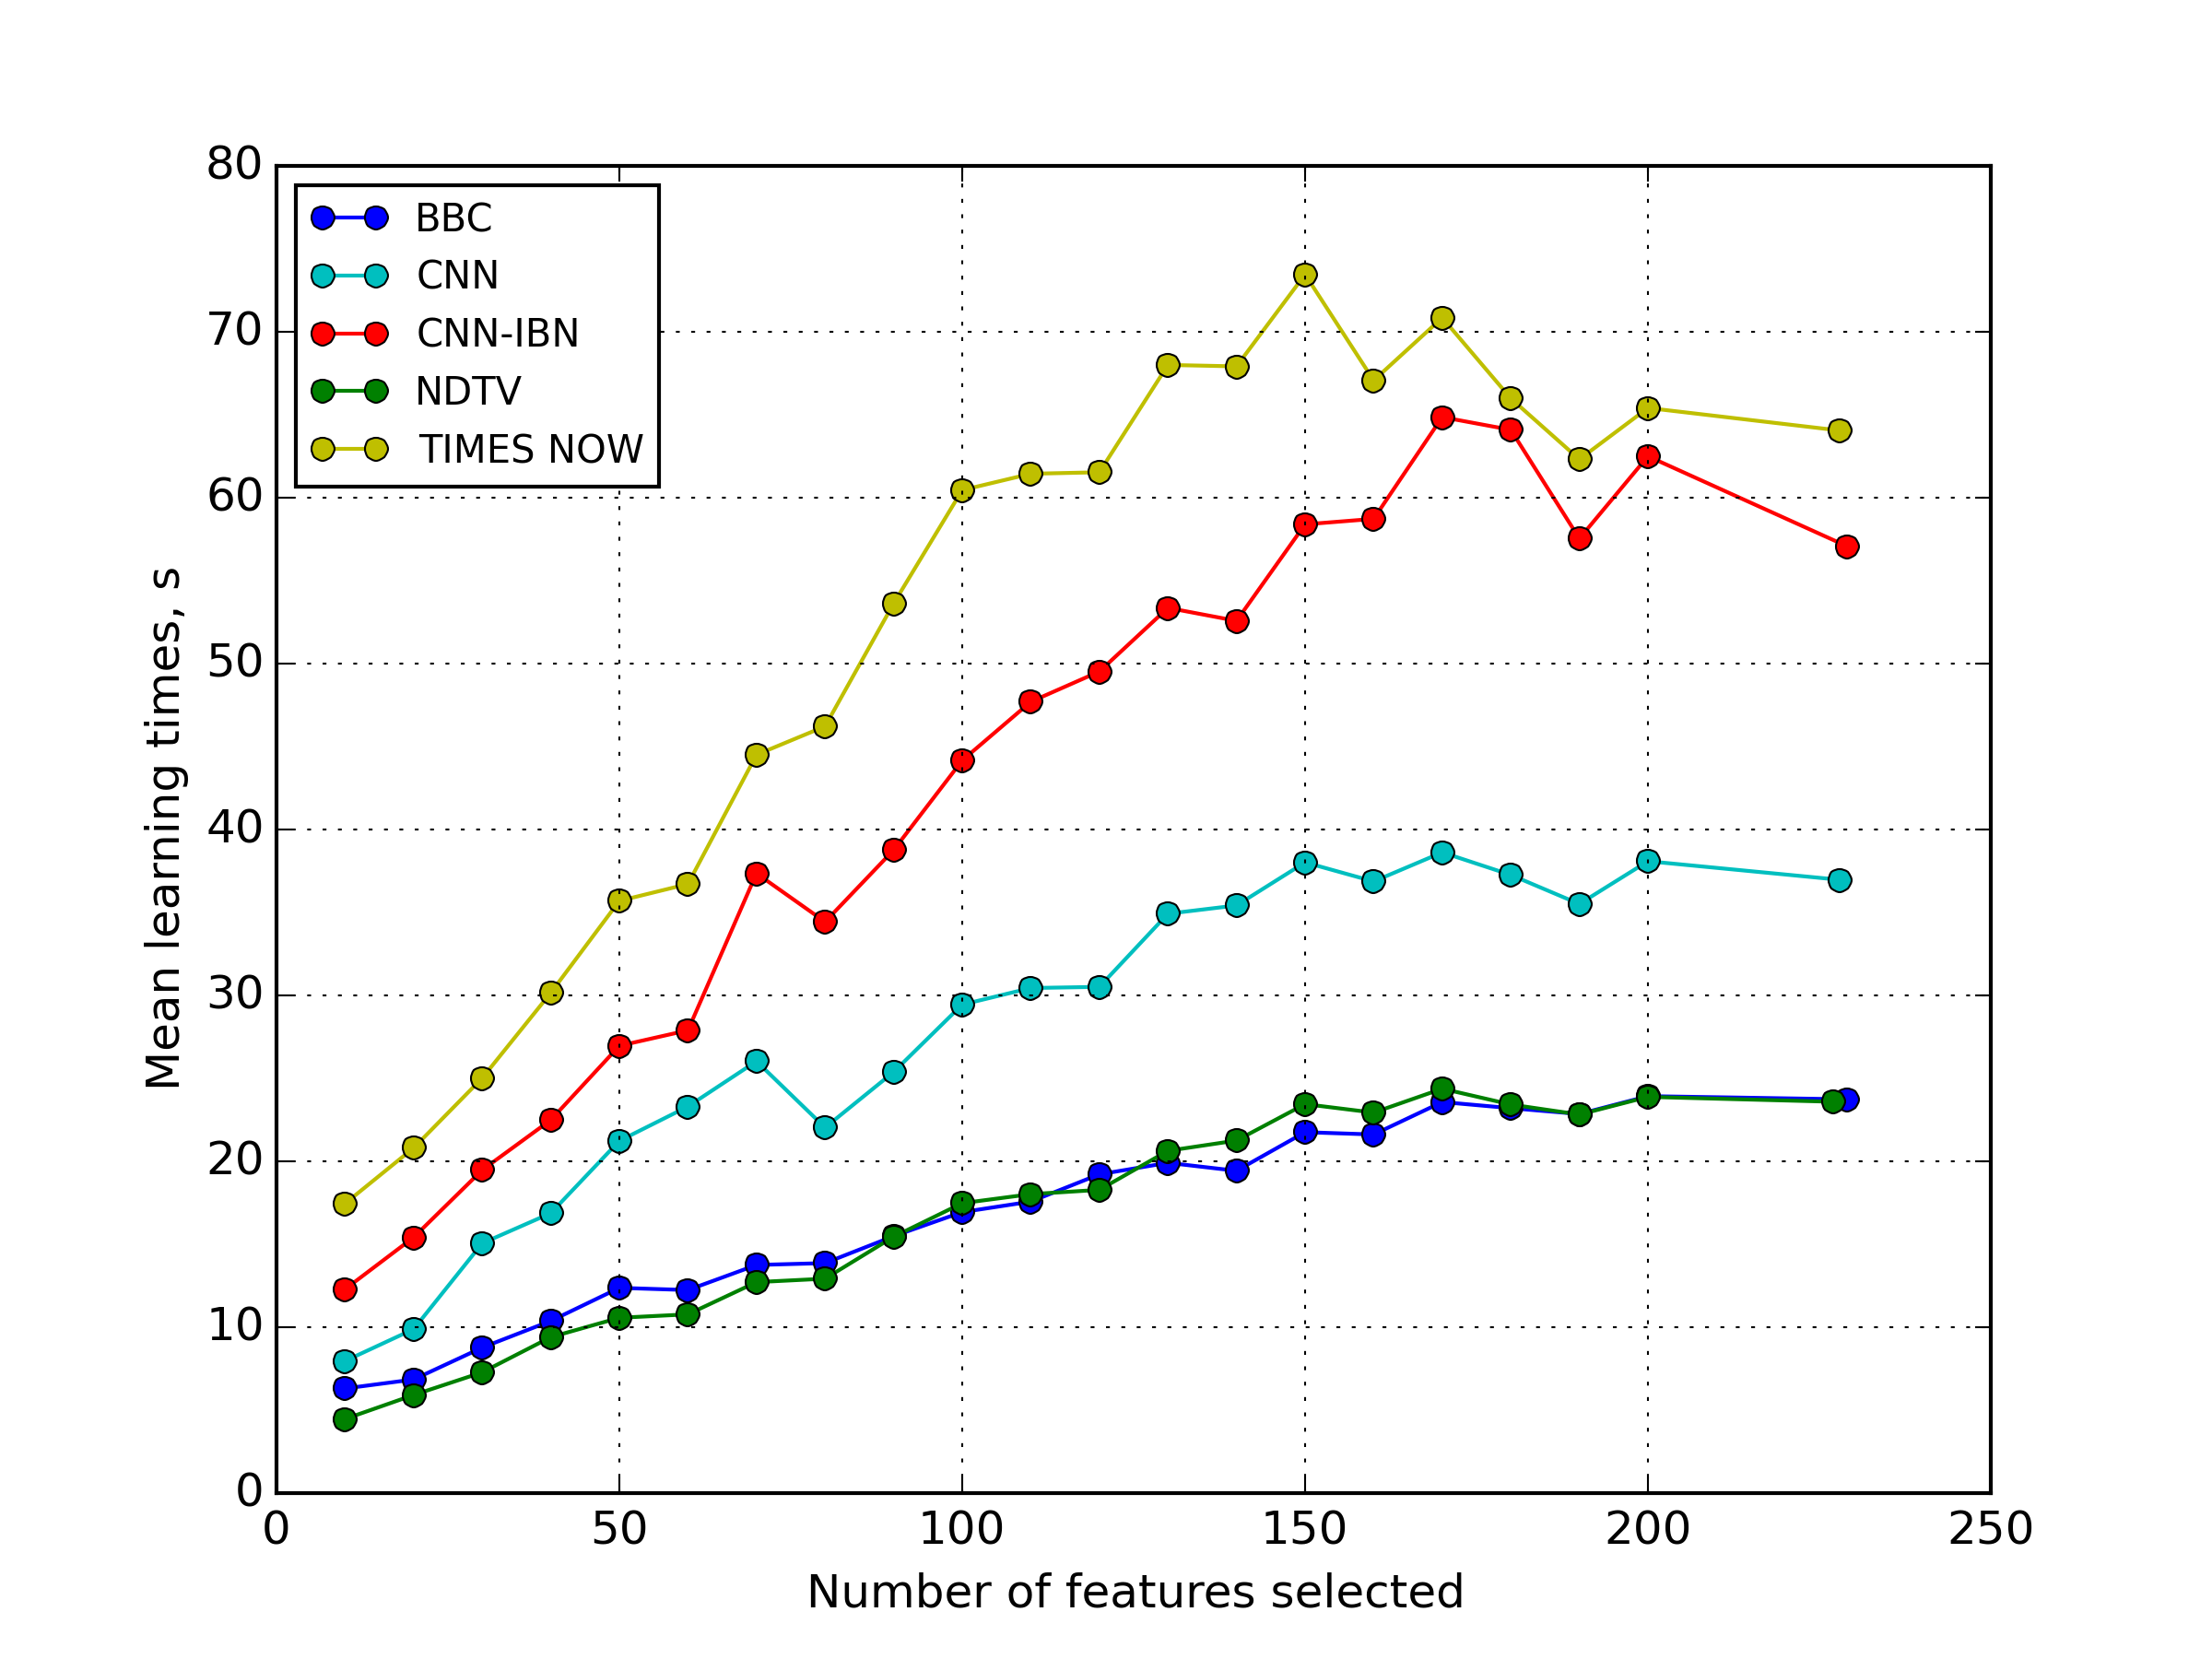
\includegraphics[width=0.5\textwidth]{images/RFS-randforestTime.png}
    \caption{Random forest learning times with RFS}
    \label{fig:randfor_rfs_times}
\end{figure} 

\par
Ситуация с градиентным бустингом деревьев решений очень похожа на ситуацию со случайным лесом: метод малочувствителен к редукции размерности.

\begin{figure}[h!]
    \centering
    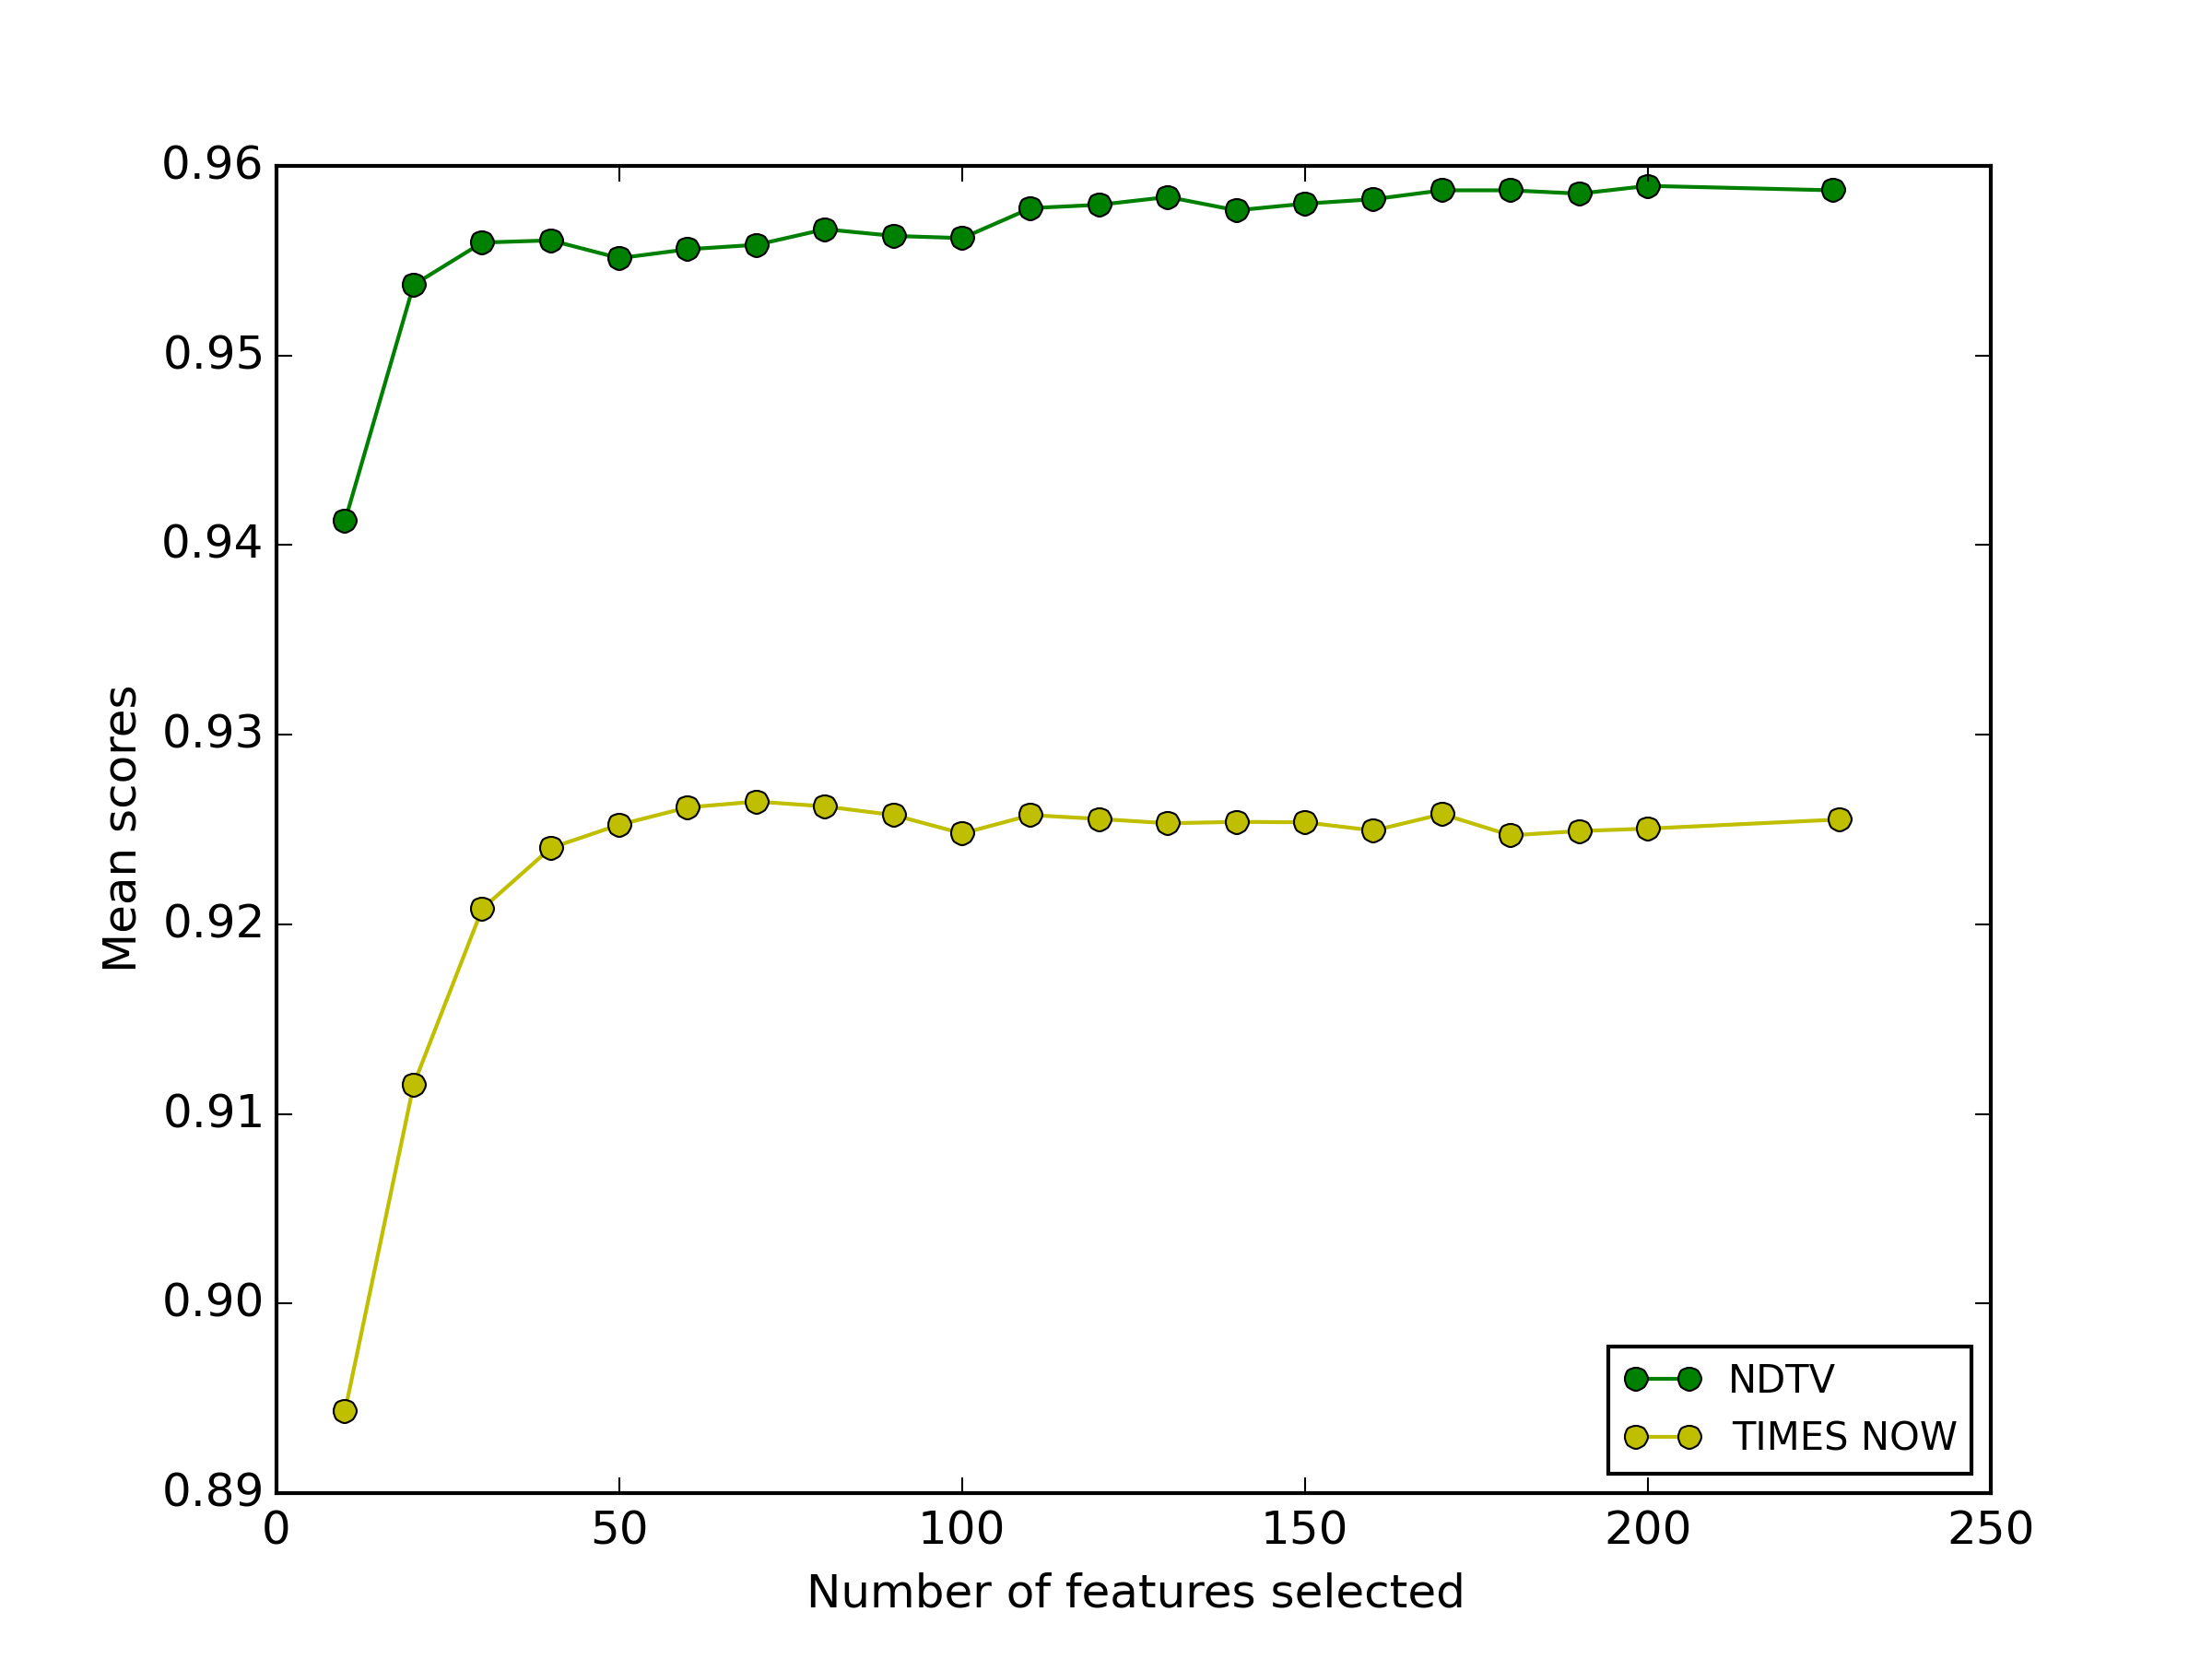
\includegraphics[width=0.5\textwidth]{images/RFS-GTB.png}
    \caption{Gradient tree boosting scores with RFS}
    \label{fig:gtb_rfs_scores}
\end{figure} 
 
 \begin{figure}[h!]
    \centering
    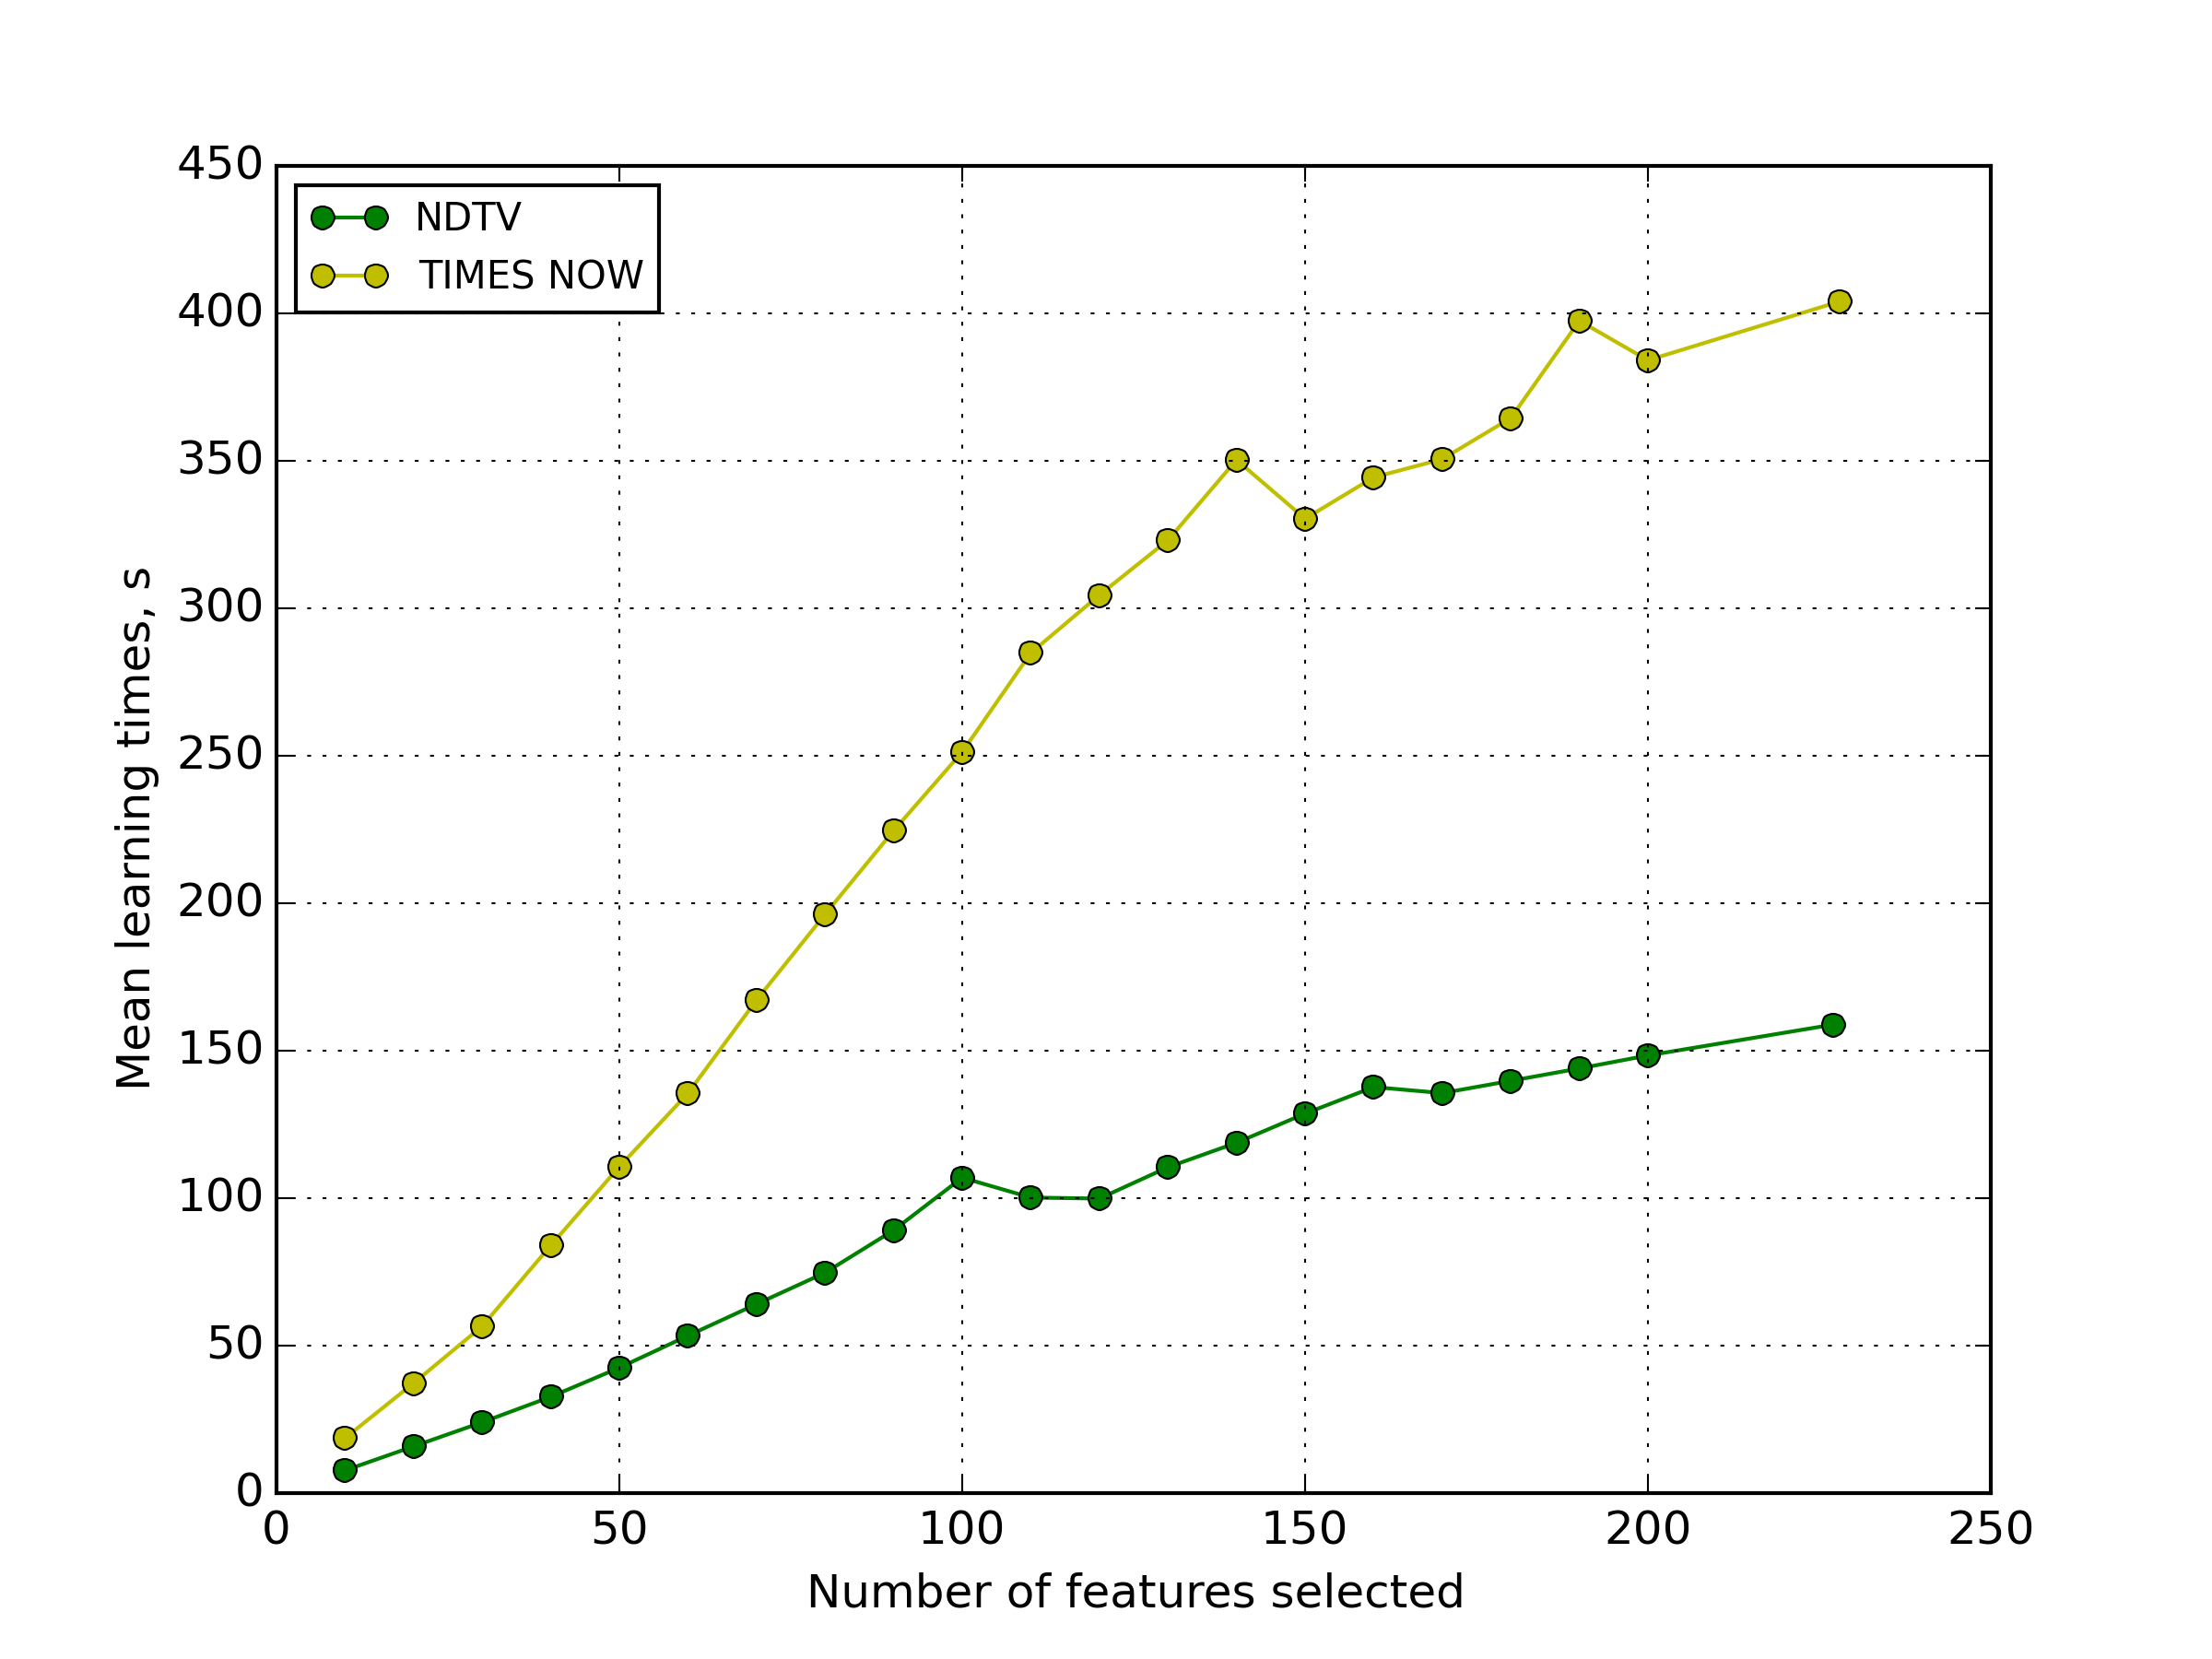
\includegraphics[width=0.5\textwidth]{images/RFS-GTBTime.png}
    \caption{Gradient tree boosting learning times with RFS}
    \label{fig:gtb_rfs_times}
\end{figure}
\par
